%\fancypagestyle{ulb_titlepage}{
%\fancyhf{}
%\renewcommand{\headrulewidth}{0pt}
%\fancyhead[L]{\includegraphics[width=\textwidth]{figures/logo_ulb-left.jpg}}}

\fancypagestyle{ulb_header_style}{
\fancyhf{}
\renewcommand{\headrulewidth}{.4pt}
%\renewcommand{\footrulewidth}{.4pt}
%\fancyhead[C]{\textbf{\Large UNIVERSIT\'{E} LIBRE DE BRUXELLES}}
\fancyhead[C]{\Large UNIVERSIT\'{E} LIBRE DE BRUXELLES}
%\fancyfoot[C]{\large Ann\'{e}e Acad\'{e}mique 2017/2018}
}

%%%%%%%%%%%%%%%% FRONTPAGE
%\pictureincenteroftextblock{figures/logo_big.png}
%\begin{titlepage}
%\thispagestyle{ulb_titlepage}
%\input{chapters/frontpage}
%\afterpage{\blankpage}
%\end{titlepage}
%%%%%%%%%%%%%%%%%%%%%%%%

\thispagestyle{ulb_header_style}
\vspace*{\fill}
\begin{center}
Facult\'{e} des Sciences\\[1.5pt]
D\'{e}partement d'Informatique \\[1.5pt]
Ann\'{e}e Acad\'{e}mique 2019/2020 \\[1cm]
Th\`{e}se pr\'{e}sent\'{e}e en vue de l'obtention du grade de Docteur en Sciences \\[2cm]
\textbf{\LARGE{ALGORITHMS AND DATA STRUCTURES FOR 3SUM AND FRIENDS}}
\end{center}

\begin{center}
\vspace{1cm}
{\large Aurélien Ooms} \\[2cm]
\end{center}

%\vspace{2cm}
\begin{center}
	Jury de th\`{e}se:
\end{center}
\begin{flushleft}
Prof.~Stefan Langerman (Université libre de Bruxelles, Président) \\
Prof.~Samuel Fiorini (Université libre de Bruxelles, Secrétaire) \\
Prof.~Jean Cardinal (Université libre de Bruxelles, Promoteur) \\
Prof.~Moshe Lewenstein (Bar Ilan University) \\
Prof.~Nabil Mustafa (ESIEE Paris)
\end{flushleft}
\vspace*{\fill}

%\afterpage{\blankpage}

\clearemptydoublepage

\fancypagestyle{plain}{
\renewcommand{\headrulewidth}{.4pt}
\fancyhf{}
\rfoot{\small\thepage}}

\pagestyle{fancy}
\fancyhf{}
\fancyhead[LE,RO]{\small\thepage}
\fancyhead[LO]{\nouppercase{\scshape\rightmark}
\renewcommand{\headrulewidth}{.4pt}}
\cfoot{}
\pagenumbering{roman}

\frontmatter
\chapternonum{To the Profane}

\todo{Cite The Restaurant at the End of the Universe by Douglas Adams. Here or
somewhere else, to illustrate what we mean by large input size.}

\todo{Avoid all technical terms here.}

QUOTE Given a set of \(n\) points in the plane \dots

FIGURE Three points on a line.

%This thesis is about problems.
Solving a problem consists in mapping a given data to an output in some
automated way.
In Computer Science, we solve problems with computers: we organize the data
with data structures, and process those structures with algorithms.
%
Solving problems consumes resources, for example, time.
Problems are considered harder if they take more resources to solve.

Geometry is about points, lines, curves, planes, surfaces, bodies, spaces \dots
We study geometric problems:
%
The given data is geometric, and the question about the data is geometric.
The proposed algorithms and data structures therefore use geometry.

This thesis studies questions about geometric problems that are simple to
formulate. However simple they are, nobody
has managed to answer them. One of the problems asks to decide, given \(n\) points in the plane,
whether three of them lie on a common line. Of course, we can solve this
problem. The question of interest here is how fast it can be solved.

It is easy to solve this problem by testing all possible candidates but that is
quite inefficient. There is a
more involved but standard construction that takes significantly less time to
execute but that is still considered inefficient. As of today, we do not know of
any reason why this problem would be any harder than sorting, which can be
solved almost as fast as the time it takes to read the data from begin to end.

Does this matter at all? It turns out simple problems appear to
be bottlenecks of more complex ones: unless we manage to improve our
understanding of the simple ones, we are stuck with inefficient solutions for
all of them.

In this thesis, we expose two novel algorithms and two novel data
structures related to the problem stated above.

\chapternonum{Token of Appreciation}

\ifdraft%
TBD
\else%
First, I wish to thank the FNRS for funding my four years of PhD with a FRIA
grant\footnote{%
Grants 5112416F and 5203818F.%
}, and ULB for providing the environment.

Second, I wish to thank my mentors, colleagues, and friends:
%
my advisor,
Jean Cardinal,
%
my professors,
Michele D'Adderio,
Samuel Fiorini,
John Iacono,
Gwenaël Joret,
Stefan Langerman,
and
Guy Louchard,
%
my colleagues at ULB,
Pierre Aboulker,
Manuel Aprile~
\includegraphics[height=1em]{figures/1f4aa},
Elena Arseneva~
\includegraphics[height=1em]{figures/1f5fe},
Luis Barba,
Yann Barsamian,
Wouter Cames van Batenburg,
Mitch Buckley,
Matthew Drescher~
\includegraphics[height=1em]{figures/1f368},
Vissarion Fisikopoulos,
Krystal Guo~
\includegraphics[height=1em]{figures/1f370},
Udo Hoffmann~
\includegraphics[height=1em]{figures/1f5a5},
Tony Huynh~
\includegraphics[height=1em]{figures/2615},
Alessandro Iraci,
Varunkumar Jayapaul,
Seungbum Jo,
Ben Karsin,
Irina Kostitsyna~
\includegraphics[height=1em]{figures/1f355},
Grigorios Koumoutsos,
Marco Macchia~
\includegraphics[height=1em]{figures/1f35d},
Keno Merckx,
Tillmann Miltzow,
Carole Muller,
Johanna Seif,
Andrew Winslow,
and
Anna Vanden Wyngaerd,
%
my coauthors,
Boris Aronov,
Ahmad Biniaz,
Jit Bose,
Sergio Cabello,
Timothy Chan,
Man-Kwun Chiu~
\includegraphics[height=1em]{figures/1f4a1},
Vida Dujmovi\'c,
Darryl Hill,
Matias Korman,
Aleksandar Markovic,
Pat Morin,
Yoshio Okamoto,
André van Renssen,
Marcel Roeloffzen,
Luís Fernando Schultz Xavier da Silveira,
Noam Solomon,
and
Sander Verdonschot,
%
and
%
totally random and awesome people like
Anthony D'Angelo~
\includegraphics[height=1em]{figures/1f39e},
Édouard Bonnet~
\includegraphics[height=1em]{figures/1f428},
Radu Curticapean~
\includegraphics[height=1em]{figures/1f1ea-1f1f9},
Daniel Gonçalves~
\includegraphics[height=1em]{figures/26f1},
Azusa Katsumizu~
\includegraphics[height=1em]{figures/1f3ef},
Rory Leisegang~
\includegraphics[height=1em]{figures/1f6b2},
and
Jules Wulms~
\includegraphics[height=1em]{figures/26f0}.
It is easy to see that I owe each and every one of you.

Finally, I wish to thank my family:
my brother, Adrien Ooms,
my father, Pierre Ooms,
my mother, Nathalie Rooseleer,
%
and
%
my cute little pumpkin, Estelle Chasseloup,
for their support and love.

\vspace{\fill}
\centerline{\LARGE GRATITUDE!}
\vspace{\fill}
\centerline{\LARGE

\includegraphics[height=1em]{figures/1f647}

\includegraphics[height=1em]{figures/1f647}

\includegraphics[height=1em]{figures/1f647}
}
\vspace{\fill}


\microtypesetup{protrusion=false}{\tableofcontents}
\microtypesetup{protrusion=true}

\addcontentsline{toc}{chapter}{Table of Contents}


\clearemptydoublepage
\mainmatter

\chapter{Bird's Eye View}

\todo{Avoid definitions at all cost.}

\todo{Roadmap link to later chapters.}

This thesis is a compilation of the contributions from four papers:
%
\begin{enumerate}
	\item[\ref{paper:ksum-algorithm}] ``\emph{Solving \(k\)-SUM Using Few Linear Queries}''~\cite{CIO16}
	\item[\ref{paper:3pol-algorithm}] ``\emph{Subquadratic Algorithms for Algebraic 3SUM}''~\cite{BCILOS19}
	\item[\ref{paper:order-type-encoding}] ``\emph{Subquadratic Encodings for Point Configurations}''~\cite{CCILO19}
	\item[\ref{paper:3sum-encoding}] ``\emph{Encoding 3SUM}''~\cite{CCILMO19}
\end{enumerate}
%
Paper~\ref{paper:ksum-algorithm} was presented at CG:YRF 16 and ESA 16.
%
Paper~\ref{paper:3pol-algorithm} was presented at EuroCG 17 and SoCG 17. It is published in DCG.
%
Paper~\ref{paper:order-type-encoding} was presented at FWCG 17, EuroCG 18, and SoCG 18. It is published in JoCG.
%
Paper~\ref{paper:3sum-encoding} was presented at EuroCG 19.

We begin this thesis with an overview of the studied topic.
%
We explain the context in which those papers were written and expose
the contributions contained in each of them.

\section*{Degeneracy Testing Problems}
%In this thesis, we
We
study \emph{Degeneracy Testing Problems}:
an instance of size \(n\) of such a problem is a single point in
high-dimensional euclidean space \(q \in \mathbb{R}^{O(n)}\). Such an instance
is called \emph{general} if and only if it passes a series of algebraic tests
(usually \(n^{O(1)}\) of them). If it fails one of the tests, it is
called \emph{degenerate}.
%
Our goal is to determine how fast an instance can be classified as general or
degenerate.

The terminology is justified because most instances
are general: the set of degenerate instances is a zero-measure subset of the
input space. It also makes sense to visualize the input space as the euclidean
space: the algebraic tests naturally induce a partition of
the input space into semialgebraic sets. Solving the problem therefore amounts
to locate the input point \(q\) in this partition of space. Our goal
is thus to determine how fast this input point can be located.

Degeneracy testing problems are easy decision problems because there are only
a finite number of candidate tests to try. The ones we study can all be solved
by brute-force in polynomial time because the number of tests is polynomial.
We show how, in some cases, this naive approach is definitely subsumed by
divide and conquer techniques exploiting the geometry of the setting.


\section*{GPT}
Let us illustrate by giving a first example of a degeneracy testing problem. We
begin with a definition:

\begin{definition}
A set of \(n\) points in \(\mathbb{R}^d\)
is in general position if and only if every (\(d+1\))-subset spans the entire
space. A point set that is not in general position is called \emph{degenerate}.
\end{definition}

The General Position Testing problem (GPT) is to decide if a given set of
\(n\) point is in general position. We can solve this problem by brute-force in
\(O(n^{d+1})\) time.
We can do it an order of magnitude faster
by constructing the dual arrangement of hyperplanes in
\(O(n^d)\) time~\cite[Theorem 24.4.1]{Hal04}.
%
On the one hand,
improving on this slightly better solution appears to be non-trivial: there
exists a class of algorithms that cannot do better even though they
exploit one of the core structures of the problem, the chirotope axioms~\cite{BLSWZ93}.
%
On the other hand, Information Theory only gives a decision tree
lower bound of \(\Omega(n \log n)\).
A popular conjecture is that no \(o(n^d)\) time real-RAM
algorithm exists for this problem.


\section*{Nonuniform Algorithms}
Another model of computation in which no \(o(n^d)\)-time algorithm for GPT
is known is the algebraic computation tree model.
%
In this model, an algorithm is a rooted tree whose internal nodes are either
arithmetic operations or sign tests on real variables, and whose leaves are the
result of the computation.
%
An execution of such an algorithm is a root-to-leaf path in the corresponding
tree.
%
The time complexity of this execution is the length of the path.

This model is
more generous than the real-RAM model in the sense that all computations that
can be carried out by only knowing the input size incur no cost.
%
Because a computation tree has a fixed size, we need a different tree for each
input size.
%
Therefore,
we say that this model is \emph{nonuniform} since it allows to have a
distinct algorithm for each input size.

This thesis considers both uniform algorithms in
the real-RAM~\cite[Section~2.3]{Sha78}
and
word-RAM~\cite{FW90}
models of computation and nonuniform algorithms
in the algebraic computation tree~\cite[Section~2]{Be83},
bounded-degree algebraic decision tree~\cite[Section~2]{SY82},
and linear decision tree~\cite[Section~2]{DL78} models of computation.
%
For a given task, the complexity of the nonuniform algorithm is less than
the complexity of the uniform algorithm.
%
While a nonuniform algorithm is rarely practical, designing those at least
means making progress on the question of whether a sensible computation tree
lower bound can be derived.


\section*{3SUM}
The 3SUM problem also falls in the category of degeneracy testing problems.
This problem asks to decide whether a given set of \(n\) numbers contains a triple
whose sum is zero. We can solve this problem by brute-force in \(O(n^3)\) time,
and in \(O(n^2)\) time with a slightly more clever algorithm.

However toyish 3SUM may look like, it is considered one of several key problems
in P: many geometric problems reduce from it in subquadratic time. Hence, a
conjectured quadratic lower bound on 3SUM implies a conditional lower bound on
all those more practical problems~\cite{GO95}.

Like for GPT, there exist lower bounds for 3SUM in restricted models of
computation: 3SUM cannot be decided in \(o(n^2)\) time if the only way we
inspect the input is by testing for the sign of weighted sums of three
input numbers~\cite{Er99a}.

Even before this lower bound was known, it was conjectured that a quadratic lower
bound would hold in other models of computation like the real-RAM model.

A first stab at the conjecture was made when it was proven that for integer
input numbers, it is possible to beat the conjectured lower bound by a few
logarithmic factors~\cite{BDP08}.
However, it remained open whether such improvements were
possible for real inputs.

Eventually, in a breakthrough paper, Gr\o nlund and Pettie gave a subquadratic
uniform algorithm that shaves a root of a logarithmic factor from quadratic
time~\cite{GP18}.
%
Since then more roots of logarithmic factors have been shaved~\cite{Fr15,GS15}.
%
To this day, it is still conjectured that, for all \(\delta > 0\), 3SUM
requires \(\Omega(n^{2 - \delta})\) time to solve in the real-RAM model.


\section*{\(k\)-SUM}
The paper of Gr\o nlund and Pettie also discusses the following generalization of
the 3SUM problem: ``For a fixed \(k\), given a set of \(n\) real numbers,
decide whether there exists a \(k\)-subset whose elements sum to zero.''
This problem is called the \(k\)-SUM problem.

Obviously, the 3SUM problem is the \(k\)-SUM problem where \(k=3\).
Moreover, there is a simple reduction from \(k\)-SUM to 2SUM when \(k\) is even
and to 3SUM when \(k\) is odd. Those reductions yield a
\(O(n^{\frac{k}{2}} \log n)\) time real-RAM algorithm for \(k\) even and a
\(O(n^{\frac{k+1}{2}})\) time real-RAM algorithm for \(k\) odd.

In their paper, in addition to the slightly subquadratic uniform algorithm for
3SUM, Gr\o nlund and Pettie give a strongly subquadratic nonuniform
algorithm for 3SUM. The algorithms runs in time \(\tilde{O}(n^{3/2})\), and,
because of the aforementioned reduction, immediately yields an improved
\(\tilde{O}(n^{\frac{k}{2}})\) nonuniform time complexity for \(k\)-SUM when
\(k\) is odd.

As for uniform time complexity we do not know whether this nonuniform
improvement can be transferred to the real-RAM model: we do not know of any
real-RAM \(o(n^{\frac{k+1}{2}})\) time algorithm for \(k\)-SUM when
\(k\) is odd.

The \(k\)-SUM problem reduces to the following point location problem: ``Given
a input point \(q \in \mathbb{R}^n\), locate \(q\) in the arrangement of
\(n \choose k\) hyperplanes of equation \(x_{i_1} + x_{i_2} + \cdots +
x_{i_k} = 0\).'' Applying the best nonuniform algorithms for point location in
arrangements of hyperplanes by Meyer auf der Heide~\cite{M84} and
Meiser~\cite{M93} yields linear decision trees of depth \(n^{O(1)}\) for
\(k\)-SUM, where the constant of proportionality in the big-oh does not depend
on \(k\).

\paragraph{Contribution 1: Paper A}
Our first contribution is a finer analysis of Meiser's algorithm
that shows that the depth of his decision tree when applied to \(k\)-SUM is
actually \(O(n^3 \log^2 n)\).  On top of that, we show how to implement a
variant of this decision tree in the real-RAM model so that its uniform running
time is \(n^{\frac{k}{2} + O(1)}\) while keeping the nonuniform running time
unchanged. Note that a naive implementation of Meiser's algorithm has a uniform
running time of \(n^{k + O(1)}\).

The approach taken by Meiser's algorithm follows the prune and search method:
Take a sample of the hyperplanes for which we do not yet know the relative
location of the input point. Locate the input point with respect to this sample
by brute-force. This amounts to identifying the cell of the sample's arrangement
which contains the input point. Refine the location of the input point in the
sample by partitioning the containing cell into low complexity subcells. Whenever
this low complexity subcell is located completely on one side of an hyperplane,
the input point is located on the same side, and so we can discard this
hyperplane without a single query to the input point. Since some hyperplanes
may intersect the low complexity subcell, rince and repeat.

The location refinement is necessary because this is the only way we can
guarantee a bound on the number of hyperplanes we have to recurse on.
Using the theory of \(\varepsilon\)-nets, we can show that, for a sample of
reasonable size, any simplex that is not intersected by a sample hyperplane
is not intersected by more than a constant fraction of the set of
hyperplanes from which the sample is drawn (with high probability). We
define the refined subcell of the algorithm presented above to be the simplex
of the bottom-vertex triangulation of the sample's arrangement that contains
the input point.


\section*{Sorting}
Before continuing, let us go back to the origins of those different problems.
The link between them will be made even clearer.

Sorting is one of the oldest and most relevant data management problems.
It is the archetypal computation tree problem.
%
Usually presented, sorting is about permutations in \emph{arrays}, but we do
not like that. We use a different abstraction:
%
Before continuing, let us go back to the origins of those different problems.
The link between them will be made even clearer.

Sorting is one of the oldest and most relevant data management problems.
It is the archetypal computation tree problem.
%
Usually presented, sorting is about permutations in \emph{arrays}, but we do
not like that. We use a different abstraction:
%
\input{text/definition/sorting}

In other words, we see the sorting problem as an information retrieval problem:
how many comparisons do we need to make in order to \emph{know} the answer to
all comparisons.
%
The usual sorting algorithms rearrange an array of input numbers into sorted
order. Another way to think about it is that they compute the permutation that
sends the input array to a sorted version of itself. This permutation is a data
structure such that given any index in the input array, we can query for the
corresponding index in the sorted array called the \emph{rank} of the element).
To retrieve the result of a comparison of two elements of the input array we can
compare their ranks in this permutation.
The usual way of defining the sorting problem restricts the data structure that
should be used to encode the \(n \choose 2\) comparisons.
The way we model the sorting problem lifts this restriction because it does not
ask to structure this information in a nice way.

The sorting problem also has its decision problem variant: Element Uniqueness.
%
\input{text/definition/element-uniqueness}

It is easy to see
that Sorting amounts to locating the point \(q\) in
the arrangement of hyperplanes of equations \(x_i - x_j = 0\)%
, and
that Element Uniqueness reduces both to and from the 2SUM
problem in linear time%
.
%
Actually, under reasonable assumptions on the computation model, sorting and
element uniqueness are the same problems: if all questions we ask about the
input are linear in the input numbers, then proving that the input
does not contain any duplicate entries requires to sort the input.
%
The same statement carries over to the \(k\)-SUM with respect to its ``sorting
version'': computing the sign of all \(n \choose k\) sums of \(k\) input
numbers.
%
Therefore, in those models of computation, the sorting problem is equivalent to
2SUM.
%
Because of this relationship between Sorting and the \(k\)-SUM problem,
we see why the better understanding of \(k\)-SUM is a natural next move.

Among all the problems this thesis touches, Sorting and Element Uniqueness
are the best understood. We know \(\Omega(n \log n)\) lower bounds in many
nonuniform models of computation and we also know a long list of simple
real-RAM algorithms for those problems whose running times match those lower
bounds. For all that matters here, those problems are solved.


In other words, we see the sorting problem as an information retrieval problem:
how many comparisons do we need to make in order to \emph{know} the answer to
all comparisons.
%
The usual sorting algorithms rearrange an array of input numbers into sorted
order. Another way to think about it is that they compute the permutation that
sends the input array to a sorted version of itself. This permutation is a data
structure such that given any index in the input array, we can query for the
corresponding index in the sorted array called the \emph{rank} of the element).
To retrieve the result of a comparison of two elements of the input array we can
compare their ranks in this permutation.
The usual way of defining the sorting problem restricts the data structure that
should be used to encode the \(n \choose 2\) comparisons.
The way we model the sorting problem lifts this restriction because it does not
ask to structure this information in a nice way.

The sorting problem also has its decision problem variant: Element Uniqueness.
%
\begin{problem}[Element Uniqueness]
	Given \(n\) numbers \(q_1, q_2, \ldots, q_n \in \mathbb{R}\),
	decide whether there exists \(1 \leq i < j \leq n\),
	such that \(q_i = q_j\).
\end{problem}


It is easy to see
that Sorting amounts to locating the point \(q\) in
the arrangement of hyperplanes of equations \(x_i - x_j = 0\)%
, and
that Element Uniqueness reduces both to and from the 2SUM
problem in linear time%
.
%
Actually, under reasonable assumptions on the computation model, sorting and
element uniqueness are the same problems: if all questions we ask about the
input are linear in the input numbers, then proving that the input
does not contain any duplicate entries requires to sort the input.
%
The same statement carries over to the \(k\)-SUM with respect to its ``sorting
version'': computing the sign of all \(n \choose k\) sums of \(k\) input
numbers.
%
Therefore, in those models of computation, the sorting problem is equivalent to
2SUM.
%
Because of this relationship between Sorting and the \(k\)-SUM problem,
we see why the better understanding of \(k\)-SUM is a natural next move.

Among all the problems this thesis touches, Sorting and Element Uniqueness
are the best understood. We know \(\Omega(n \log n)\) lower bounds in many
nonuniform models of computation and we also know a long list of simple
real-RAM algorithms for those problems whose running times match those lower
bounds. For all that matters here, those problems are solved.


\section*{A Zoo of Generalizations}
Obviously, the \(k\)-SUM problem is not the only possible way to generalize
Sorting.

Hopcroft's problem asks whether given \(n\) points and \(n\) hyperplanes in
\(\mathbb{R}^d\), one of the points lies on one of the hyperplanes. When
\(d=1\), this problem is Element Uniqueness. Finding the location
(``above''/``below'')
of each point with respect to each hyperplane generalizes Sorting.

The dominance reporting problem asks, given \(n\) points in \(\mathbb{R}^d\),
to report all pairs of points such that the first dominates the other in all
dimensions. Once again, for \(d=1\), this problem is Sorting because it asks
for the answer to all comparisons of the type \(p_i \leq q_i\).

Sorting \(X+Y\) is also a canonical problem in \(P\): given two sets
\(X\) and \( Y \) of \( n \) numbers each, sort the set \( \{\, x + y \colon\,
x \in X, y \in Y\,\} \). Sorting \(X+Y\) reduces linearly to the sorting
version of 4SUM because it asks for the sign of all comparisons of the type
\(x+y \leq x'+y'\).

We already saw that GPT and Sorting belong to the same family of
high-dimensional point location problems. There is a good reason for that: when
\(d=1\), GPT is Element Uniqueness. In one-dimensional space, GPT
asks whether any two points are the same. Picturing this space as
the (horizontal) real line, we see that the ``sorting version'' of GPT asks to
compute for each pair of points which one is on the ``left'' of the other which
simply amounts to Sorting the one-dimensional input points.


%\section*{SUBSET-SUM}
%Note that the unparameterized version of \(k\)-SUM is the SUBSET-SUM problem,
%which is NP-complete... Discuss nonuniform polytime algo.

%Because of that, we put Sorting and Element Uniqueness as problems at the
%origin of a zoo of problems.

\todo{Mention Moshe and Chan's paper at some point and show how it applies to
other fields (string indexing).}

\section*{Intermediate Problems}
A perspicacious reader may have frowned at the previous paragraphs wondering
whether this embryo of classification brings more insight than confusion.
``Sure!'', one may say, ``Many problems involve sorting, and therefore,
according to this dubious definition, are generalizations of it.''

However, the author begs to differ.

As a first example, take one of the best known algorithms for 3SUM. This
algorithm reduces an instance of 3SUM to a sorting phase and a searching
phase~\cite{GP18}. The sorting phase consists in answering all questions of the type
\( x_i + x_{i'} \le x_j + x_{j'} \) with some restriction on the indices.
Well, it
turns out that this phase is exactly an instance of
the sorting version of the 2SUM problem where the input numbers are the
differences \(x_i - x_j\).\footnote{This observation generalizes to the \(k\)-SUM
problem: any \(k\)-SUM instance can be reduced to a larger (\(k-1\))-SUM instance
followed by a searching phase.} Moreover, to make the uniform algorithm
practical, they implement the resolution of the 2SUM instance via dominance
reporting.
Note that this sorting problem is similar to the Sorting \(X+Y\) problem where
the answers to most questions are not cared for.

As a second example, we have the GPT problem. For this problem, the fact that
the one-dimensional version is Sorting does not seem to give any insight on how
to apprehend the more general problem, even in two dimensions. In order to make
some progress in that direction, we need to capture more precisely to which
family of problems GPT belongs. For that, we look at the algebra behind the
problem.

GPT asks whether for any choice of \(n \choose d+1\) input points \(p_i\) with
coordinates \((p_{i,1} , p_{i,2} , \ldots, p_{i,d} )\),
the determinant
%
\begin{displaymath}
  \det\begin{pmatrix}
    1 & p_{1,1} & p_{1,2} & \hdots & p_{1,d} \\
    1 & p_{2,1} & p_{2,2} & \hdots & p_{2,d} \\
    \vdots & \vdots & \vdots & \ddots & \vdots \\
    1 & p_{d+1,1} & p_{d+1,2} & \hdots & p_{d+1,d}
  \end{pmatrix}
\end{displaymath}
is zero. This determinant is a degree-\(d\) (\(d^2 + d\))-variate polynomial.
In particular, when \(d=2\), the determinant is a degree-\(2\) \(6\)-variate
polynomial. The GPT testing problem then amounts to testing whether the
coordinates of any combination of the input points yields a root of that
polynomial. We therefore consider the more general \(d\)-dimensional-\(k\)-POL
(\(d\)D-\(k\)-POL) problem:
%
Given a \(dk\)-variate constant degree polynomial \(F\) and a set \(S\) of \(n\) points
in \(\mathbb{R}^d\), decide whether \(F(S^k)\) contains any zeroes.
%
For instance, 2D-3POL generalizes GPT with \(d=2\) where the constant degree
polynomial is the \(3 \times 3\) determinant mentioned above. Moreover, 1D-3POL
generalizes 3SUM where the polynomial is simply the sum function. Equally
interesting is the fact that 2D-2POL generalizes Hopcroft's problem with
\(d=2\) where the polynomial is the dot product.

\paragraph{Contribution 2: Paper B}
In paper B, we generalize Gr\o nlund and Pettie's approach to solve 1D-3POL (or
more simply, 3POL) in subquadratic time. Our approach is essentially the same
in that it reduces 3POL to a sorting phase and a searching phase, the sorting
phase being an instance of 2D-2POL.\footnote{Note that according to the implied
definition, \(d\)D-\(k\)-SUM is equivalent to \(k\)-SUM. Therefore, the 2SUM
instance in the sorting phase of their 3SUM algorithm is an instance of 2D-2SUM
in disguise.} Again, the implementation of the uniform algorithm solves this
instance of 2D-2POL using dominance reporting (a generalization of it).

This result illustrates why a better understanding of the landscape of problems
surrounding GPT helps to identify intermediate problems whose resolution marks
progress towards the question of whether GPT admits subquadratic algorithms.
%
Figure~\ref{fig:landscape} depicts this landscape.

\begin{figure}
  \centering{}
  \includegraphics[width=\linewidth]{figures/landscape}
  \caption{%
	The decision problems surrounding GPT.
	%
	Arrows indicate linear time reductions. \(A = B\) indicates that
	\(A\) and \(B\) are the same problems and \(A \simeq B\) indicates that
	\(A\) is the identification variant of \(B\).
	%
	Known upper bounds are indicated next to the problem's name.
	%
	When the uniform and nonuniform upper bounds differ, we place the best
	uniform upper bound on the right.
	%
	Solid lines indicate apparent time-complexity differences between the best
	known nonuniform algorithms.
	%
	Dotted lines indicate apparent
	time-complexity differences between the best known uniform algorithms.%
  }%
  \label{fig:landscape}
\end{figure}


\section*{Encodings}
Naive algorithms for Element Uniqueness, 3SUM, and \(k\)-SUM would search
all possible combinations of \(2\), \(3\), or \(k\) input numbers for a match
and reach horrible running times: respectively \(O(n^2)\), \(O(n^3)\), and \(O(n^k)\).

The way better uniform algorithms for those problems work
is by a combination of sorting and searching. The sorting part
constructs a data structure and the searching part uses this data structure to
answer the question at hand. The achieved running time is a balance between the
cost of sorting and the cost of searching. This results in better
running times than the naive ``search only'' solutions.

For instance, an efficient algorithm for the
Element Uniqueness problem would first sort the input, then scan it for
duplicates among adjacent numbers in this sorted order. The data structure that
is constructed is the permutation we talked about earlier. This structure
achieves a good compressing ratio by encoding the answer to all \(O(n^2)\)
pairwise comparisons of two input numbers in \(O(n \log n)\) bits.

For this reason Element Uniqueness is comparatively simpler than the 3SUM and
\(k\)-SUM problems.
For a nonuniform algorithm, constructing this structure is sufficient to solve
the problem: Once the construction is over, we can discard the input because
all the information we need is encoded in the data structure. Since the nonuniform
models of computation we consider do not care about computations not involving
the input, the searching part does not cost anything.

The case of 3SUM and \(k\)-SUM is more complex: The sorting phase only encodes
a fraction of all possible queries. This leaves a significant amount of work
for the searching phase. Therefore, both the sorting phase and the searching
phase contribute to the nonuniform cost of those algorithms.

The case of GPT is also interesting. The naive algorithm queries
\(O(n^{d+1})\) input tuples while the better algorithm constructs the dual
arrangement in \(O(n^d)\) time.
As in the case of Element Uniqueness,
this dual arrangement is the data structure that encodes the answer to all
\(O(n^{d+1})\) queries while achieving a significant space gain.

While the goal sought in the design of algorithms is to find the best possible
balance between those sorting and searching phases, a different question becomes
evident: ``What is the most resource efficient data structure encoding all the
combinatorial information carried by the input?''. For this question, resource
efficiency can be measured in three ways: space requirements, construction
time, and query time. If one only cares about space, a trivial answer
points its head out: if there are only \(X\) combinatorial types then each type
can be encoded with \(\lceil \log X \rceil\) bits. However, this solution is
unlikely to yield good construction time or good query time.

In the case of Element Uniqueness, this question has been answered long ago.
Sorting the input in \(O(n \log n)\) time will construct a permutation using
\(O(n \log n)\) bits that can be queried for any pairwise comparison in
\(O(1)\) time. However, the question is still widely open for
3SUM, \(k\)-SUM, and GPT.

In paper C we design the first subquadratic space data structure for encoding
the combinatorial type of a two-dimensional GPT instance. This data structure
can be constructed in quadratic time and queries are answered in sublogarithmic
time. Those results can be adapted to work for higher-dimensional GPT to yield
sub-\(O(n^d)\) space data structures with good construction and query times.

Since 3SUM reduces to GPT, the results of paper C can be applied to encode the
combinatorial type of 3SUM instances. However, since 3SUM is much better
understood than GPT we should aim for better encodings. This is exactly what we
do in paper D. By filling the gaps in the partial data structure
used in Gr\o nlund and Pettie's algorithm~\cite{GP18}, we design an encoding
that uses \(O(n^{3/2} \log n)\) bits, can be constructed in \(O(n^2)\) time and
answers queries in constant time.

\todo{Conclude with remark on encodings derived from decision trees.}

\paragraph{Contribution 3: Papers C \& D}
In Paper~\ref{paper:order-type-encoding} we design the first subquadratic space
data structure for encoding the combinatorial type of a two-dimensional GPT
instance. This data structure can be constructed in quadratic time and queries
are answered in sublogarithmic time. Those results can be adapted to work for
higher-dimensional GPT to yield \(o(n^d)\)-space data structures with good
construction and query times.

Since 3SUM reduces to GPT, the results of Paper~\ref{paper:order-type-encoding}
can be applied to encode the combinatorial type of 3SUM instances. However,
since 3SUM is much better understood than GPT we should aim for better
encodings. This is exactly what we do in Paper~\ref{paper:3sum-encoding}.
By filling the gaps in the partial data structure used in Gr\o nlund and
Pettie's algorithm~\cite{GP18}, we design an encoding that uses \(O(n^{3/2}
\log n)\) bits, can be constructed in \(O(n^2)\) time and answers queries in
constant time.


\section*{The Secret Ingredient}
What makes the success of our methods are now-standard geometric
divide-and-conquer tools: \(\varepsilon\)-nets and cuttings.

The idea of an \(\varepsilon\)-net is simple, yet powerful. Given a set of
\(m\) hyperplanes in \(\mathbb{R}^d\), construct a sample of those hyperplanes
of size \(f(d, \varepsilon)\) uniformly at random. Then, with high probability,
any simplex that is not intersected by an hyperplane of the sample is intersected
by at most \(\varepsilon m\) hyperplanes of the original set. The sample is
called a \emph{net} because it does not let the fat simplices through: a
simplex intersected by more than \(\varepsilon m\) hyperplanes must be intersected
by one of the sample.
%
This yields an efficient point location tool: construct a sample, find the cell
of its arrangement that contains the query point, find the simplex of its
triangulation that contains the query point, and recurse on the fraction of
hyperplanes that intersect it.

Triangulate the whole arrangement of the sample and you get an
\(\varepsilon\)-cutting: a partition of space into simplices such
that each simplex is intersected by at most \(\varepsilon m\) hyperplanes.
We use cuttings in applications where multiple queries are made on the same set
of hyperplanes.


\section*{Wrapping it up}
Since publication of those papers, a few developments have surfaced.

Ezra and Sharir~\cite{ES17} show how trading simplices of the bottom-vertex
triangulation for prisms of the vertical decomposition in Meiser's algorithm
yields a shallower decision tree of depth \(O(n^2 \log n)\). Essentially, the
improvement over our result in Paper~\ref{paper:ksum-algorithm}
lies in the fact that, for vertical decomposition, the sample size can be taken
to be an order of magnitude smaller.

%All nonuniform algorithm for \(k\)-SUM we have mentioned query the input with
%\(s\)-linear queries: a \(s\)-linear query asks for the sign of weighted sums of
%\(s\) input numbers. A decision tree that queries the input exclusively with
%\(s\)-linear queries is called a \(s\)-linear decision tree.

%The nonuniform algorithm of Gr\o nlund and Pettie for
%\(k\)-SUM with \(k\) odd uses many more queries than the methods of Meyer auf der
%Heide and Meiser. However, its merit lies in that it only asks very simple
%questions about the input: this algorithm probes the input
%with (\(2k-2\))-linear queries while the others use \(n\)-linear queries.

In a breakthrough paper, Kane, Lovett, and Moran~\cite{KLM18} give a
linear decision tree of depth \(O(n \log^2 n)\) for \(k\)-SUM, almost
matching the \(\Omega(n \log n)\) lower bound. This improves both on
Paper~\ref{paper:ksum-algorithm} and Ezra and Sharir~\cite{ES17}.

In~\cite{Ch18}, Chan shaves more logarithmic factors from the time complexity
of uniform algorithms for 3SUM and 3POL. While we focused on applications that solve
3SUM-hard geometric problems with one-dimensional input in
Paper~\ref{paper:3pol-algorithm}, he shows how
the ideas that work for 3POL also work for some 3SUM-hard geometric problems
with two-dimensional data.



\clearemptydoublepage
\renewcommand{\sectionmark}[1]{\markright{#1}}
\renewcommand{\chaptermark}[1]{\markboth{#1}{}}
\fancyhead[LE,RO]{\small\thepage}
\fancyhead[RE]{\nouppercase{\scshape\thesection.\ \rightmark}}
\fancyhead[LO]{\nouppercase{\scshape\thechapter.\ \leftmark}}

\clearemptydoublepage
\chapter{Models of Computation}
\chapter{Decision Trees for $k$-SUM}
\label{chapter:ksum-algorithm}

Given three sets of \(n\) real numbers
\(A = \{\, a_1 < a_2 < \cdots < a_n\,\} \),
\(B = \{\, b_1 < b_2 < \cdots < b_n\,\} \),
and \(C = \{\, c_1 < c_2 < \cdots < c_n\,\}\),
we wish to build a discrete data structure (using bits, words, and pointers) such that,
given any triple \((i,j,k) \in {[n]}^3\) it is possible to compute the sign of
\(a_i + b_j + c_k\) by only inspecting the data structure (we cannot consult
\(A\), \(B\), or \(C\)).
We refer to the map $\chi : {[n]}^3\to \{-,0,+\}, (i,j,k)\mapsto\mathrm{sgn}
(a_i+b_i+c_k)$ as the {\em 3SUM-type} of the instance $\langle A,B,C \rangle$.
Obviously, one can simply construct a lookup table of size \(O(n^3)\), such
that triple queries can be answered in \(O(1)\) time. We aim at improving on
this trivial solution.

In the 3SUM problem, we are given an array of numbers as input and are asked
whether any three of them sum to 0. In the mid-nineties, this problem was
identified as a bottleneck of many
important problems in geometry, such as detection of affine degeneracies or
motion planning~\cite{GO95}. Since then, it has become a central problem in
fine-grained complexity theory~\cite{PW10}. It has long been conjectured to
require $\Omega (n^2)$ time. In 2014, it was shown to be solvable in $o(n^2)$
time, but no algorithm with running time $O(n^{2-\delta})$ with constant
$\delta>0$ is known~\cite{GP18}.

Lower bounds exist in restricted models of computation. Most notably,
$\Omega(n^2)$ 3-linear queries are needed to solve 3SUM~\cite{Er99a},
and nontrivial lower bounds have also been proven for slightly more powerful linear
decision trees~\cite{AC05}. However, in a recent breakthrough contribution, Kane, Lovett,
and Moran showed that 3SUM could be solved using $O(n\log^2 n)$
6-linear queries~\cite{KLM18}, hence within a $O(\log n)$ factor of the
information-theoretic lower bound.

Linear decision trees are examples of {\em nonuniform algorithms}, in which we
are allowed to have different algorithms for different input sizes.
Algebraic decision trees generalize linear decision trees
by allowing decision based on the sign of constant-degree polynomials at each
node~\cite{SY82}.

Any decision tree identifying the 3SUM-type of a 3SUM instance yields a concise
encoding of this 3SUM-type:
just write down the outcome of the successive tests. Knowing the decision tree
by convention, this sequence of bits is
sufficient to recover the sign of any triple.

The question we consider here is how to make such a representation efficient,
in the sense that not only does it use merely a few bits, but the answer to any
triple query can be recovered efficiently. Understanding the interplay between
nonuniform algorithms and such data structures hopefully sheds light on the
intrinsic structure of the problem.

\paragraph{Contribution}

As there are only $O(n^3)$ queries, a table
of size $(\log_2 3) n^3 + O(1)$ bits suffices to give constant query time
\cite{DPT10}. This can be improved to $O(n^2\log n)$ bits of space by
storing for each pair $(i,j)$ the values
\(k_<(i,j) = \max \{ 0\}\cup \{k \colon\, a_i + b_j + c_k < 0\}\) and
\(k_>(i,j) = \min \{ N+1\}\cup \{k \colon\, a_i + b_j + c_k > 0\}\).
For a query \((i,j,k)\), we compare \(k\) against the values \(k_<(i,j)\) and \(k_>(i,j)\)
to recover \(\chi(i,j,k)\) in \(O(1)\) time. All \(k_<(i,j)\) and \(k_>(i,j)\)
can be computed in \(O(n^2)\) time via the classic quadratic time algorithm for
3SUM.
%: if \(k \leq k_<(i,j)\), then \(\chi(i,j,k)=-1\), if \( k_<(i,j)< k < k_>(i,j)\),
%then \(\chi(i,j,k)=0\), and if \( k_>(i,j)\leq k\), then \(\chi(i,j,k)=+1\).
%The representation takes \( O(n^2 \log N \) bits, and each query can be answered by comparing
%pairs of indices, which takes \(O(1)\) time.

One seemingly simple representation is to store the numbers in $A$, $B$ and
$C$; however these are reals and thus we need to make them representable using
a finite number of bits.
In \S\ref{s:numbers} we show that a minimal integer representation of a
3SUM instance may require $\Theta(n)$ bits per value, which would give
rise to a $O(n)$ query time and $O(n^2)$ space, which is far from
impressive.
In \cite{CCILO18} the problem of given a set of $N$ lines, to create an
encoding of them so that the orientation of any triple (the \emph{order type})
can be determined was studied; our problem is a special case of this where the
lines only have three slopes.
Can we do better for the case of 3SUM? We answer this in the affirmative.
In \S\ref{s:space} we show how to use an optimal $O(n \log n)$ bits of
space with a polynomial query time. Finally, in section~\ref{s:sscqt} we show
how to use $\tilde{O}(n^{3/2})$ space to achieve $O(1)$-time queries.

\section{Sorting}

QUOTE ``Please, pretty please, order those data from smallest to largest''.

The sorting problem is one of the oldest and most practical data management
problems.
%
Usually, sorting is about permutations in \emph{arrays}, but we do not like
that. We use a different abstraction:

\input{text/definition/sorting}

Without any

\subsection{Algorithms}
Explain models of computation: uniform nonuniform etc

\subsection{Data Structures}

Most (if not all) algorithms for sorting receive their input data as a list and
output their answer as a permutation of this data. This permutation is a
compact data structure: the structure takes space proportional to the minimum
amount of space possible (about \(\log_2 n!\)), and the answer to each
comparison can be retrieved instantly from the structure.


\section{The \(k\)-SUM Problem}

The \(k\)-SUM problem is simple enough: given a list of \(n\) real numbers,
decide whether \(k\) of them sum to zero.

\input{text/definition/ksum}

For fixed \(k\), the \(k\)-SUM problem can be solved in polynomial time
\(O(n^k)\) by testing all possible candidate solutions.
The interesting question is whether it is possible to improve on
this brute-force solution.

The \(k\)-SUM problem is defined as follows: given a collection of $n$ real
numbers decide whether any $k$ of them sum to zero, where $k$ is a constant.
It is a fixed-parameter version of the subset-sum problem, a standard \textit{NP}-complete
problem. The \(k\)-SUM problem, and in particular the special case of 3SUM,
has proved to be a cornerstone of the fine-grained complexity program aiming at
the construction of a complexity theory for problems in $P$. In particular,
there are deep connections between the complexity of \(k\)-SUM, the Strong
Exponential Time Hypothesis~\cite{PW10,CGIMPS15}, and the complexity of many
other major problems in
$P$~\cite{GO95,BH99,MO01,P10,ACLL14,AVW14,GP14,KPP14,ALW14,AWY15,CL15}.

It has been long known that the \(k\)-SUM problem can be solved in time
$O(n^{\frac{k}{2}}\log n)$ for even $k$, and $O(n^{\frac{k+1}{2}})$ for odd
$k$. Erickson~\cite{Er99} proved a near-matching lower bound in the $k$-linear
decision tree model. In this model, the complexity is measured by the depth of
a decision tree, every node of which corresponds to a query of the form
$q_{i_1} + q_{i_2} + \cdots + q_{i_k} \ask{\le} 0$, where $q_1, q_2, \ldots, q_n$ are the
input numbers. In a recent breakthrough paper, Gr\o nlund and
Pettie~\cite{GP14} showed that in the $(2k-2)$-linear decision tree model,
where queries test the sign of weighted sums of up to $2k-2$ input numbers, only
$O(n^\frac{k}{2}\sqrt{\log n})$ queries are required for odd values of $k$. In
particular, there exists a $4$-linear decision tree for 3SUM of depth
$\tilde{O}(n^\frac{3}{2})$ (here the notation $\tilde{O}$ ignores polylogarithmic
factors), while every 3-linear decision tree has depth $\Omega
(n^2)$~\cite{Er99}. This indicates that increasing the size of the queries,
defined as the maximum number of input numbers involved in a query, can yield
significant improvements on the depth of the minimal-height decision tree. Ailon and
Chazelle~\cite{AC05} slightly extended the range of query sizes for which a
nontrivial lower bound could be established, elaborating on Erickson's
technique.

It has been well established that there exist nonuniform
polynomial-time algorithms for the subset-sum problem. One of them was
described by Meiser~\cite{M93}, and is derived from a data structure for point
location in arrangements of hyperplanes using the bottom vertex decomposition.
This algorithm can be cast as the construction of a linear decision tree in which
the queries have non-constant size.

\subsection{Our results}
In Section~\ref{sec:query-complexity}, we show the existence of an $n$-linear
decision tree of depth $\tilde{O}(n^3)$ for \(k\)-SUM using a careful
implementation of Meiser's algorithm~\cite{M93}.
Although the high-level algorithm itself is not new, we refine the
implementation and analysis for the \(k\)-SUM problem.%
\footnote{After submitting this manuscript, we learned from a personal communication
with Herv\'e Fournier that a similar analysis for arbitrary hyperplanes appears in his PhD
thesis~\cite{F01} (in French).}
Meiser presented his algorithm as a general method of point location in $m$
given $n$-dimensional hyperplanes that yielded a $\tilde{O}(n^4 \log
m)$-depth algebraic computation tree; when viewing the \(k\)-SUM problem as a point
location problem, $m$ is $O(n^k)$ and thus Meiser's algorithm can be viewed
as giving a $\tilde{O}(n^4)$-depth algebraic computation tree.
We show that while the
original algorithm was cast as a nonuniform polynomial-time algorithm,
it can be implemented in the linear decision tree model with an
$\tilde{O}(n^3)$ upper bound.
Moreover, this result implies the same improved upper bound on the depth of
algebraic computation trees for the $k$-SUM problem,
as shown in Appendix~\ref{app:act}.

There are two subtleties to this result. The first is inherent to the chosen
complexity model: even if the number of queries to the input is small (in
particular, the degree of the polynomial complexity is invariant on $k$), the
time required to \emph{determine which queries should be performed} may be
arbitrary. In a na\"ive analysis, we show it can be trivially bounded by
$\tilde{O}(n^{k+2})$. In Section~\ref{sec:time-complexity} we present an algorithm to
choose
which decisions to perform whereby the running time can be reduced to
$\tilde{O}(n^{\frac{k}{2}+8})$. Hence, we obtain an
$\tilde{O}(n^{\frac{k}{2}+8})$ time randomized algorithm in the RAM model
expected to perform $\tilde{O}(n^3)$ linear queries on the input\footnote{%
	Gr{\o}nlund and
	Pettie~\cite{GP14} mention the algorithms of Meyer auf der Heyde~\cite{M84} and
	Meiser~\cite{M93}, and state ``(\ldots) it was known that all \(k\)-LDT problems
	can be solved by $n$-linear decision trees with depth $O(n^5\log
	n)$~\cite{M93}, or with depth $O(n^4\log (nK))$ if the coefficients of the
	linear function are integers with absolute value at most $K$~\cite{M84}.
	Unfortunately these decision trees are not efficiently constructible. The
	time required to determine \emph{which} comparisons to make is
	exponential.'' We prove that the trees can have depth $\tilde{O}(n^3)$ and
	that the whole algorithm can run in randomized polynomial-time.}.

The second issue we address is that the linear queries in the above algorithm may
have size $n$, that is, they may use all the components of the input.
The lower bound of Erickson shows that if the queries are of minimal size, the number
of queries cannot be a polynomial independent of $k$ such as what we obtain, so
non-minimal query size is clearly essential to a drastic reduction in the number of queries needed.
This gives rise to the natural question as to what is the relation between query size and number of queries.
In particular, one natural question is whether queries of size less than $n$
would still allow the problem to be solved using a number of queries that is a
polynomial independent of $k$. We show that this is possible; in Section~\ref{sec:query-size},
we introduce a range of
algorithms exhibiting an explicit tradeoff between the number of queries and
their size. Using a blocking scheme, we show that we can restrict to
$o(n)$-linear decision trees. We also give a
range of tradeoffs for $O(n^{1-\alpha})$-linear decision trees. Although the
proposed algorithms still involve nonconstant-size queries, this is
the first time such tradeoffs are explicitly tackled. Table~\ref{tab:results} summarizes our results.

\begin{table}
\centering
\caption{Complexities of our new algorithms for the \(k\)-SUM problem. The query
size is the maximum number of elements of the input that can be involved in a
single linear query. The number of blocks is a parameter that allows us to
change the query size (see Section~\ref{sec:query-size}).
The origin of the constant in the exponent of the time complexity is due to
Lemma~\ref{lem:bound}. We conjecture it can be reduced, though substantial
changes in the analysis will likely be needed to do so.}
\label{tab:results}
\begin{tabular}{|c|c|c|c|c|}
	\hline

	& \# blocks & query size & \# queries & time \\
	\hline
	Theorem~\ref{thm:cube} &
	$1$ &
	$n$ &
	$\tilde{O}(n^3)$ & $\tilde{O}(n^{\lceil\frac{k}{2}}+8\rceil)$
	\\

	\hline

	Theorem~\ref{thm:query-size} &
	$b$ &
	$k\lceil\frac{n}{b}\rceil$ &
	$\tilde{O}(b^{k-4}n^3)$ &
	$\tilde{O}(b^{\lfloor\frac{k}{2}}-9\rfloor n^{\lceil\frac{k}{2}}+8\rceil)$
	\\

	\hline

	Corollary~\ref{cor:logn} &
	$b=\Theta(\polylog(n))$ &
	$o(n)$ &
	$\tilde{O}(n^3)$ &
	$\tilde{O}(n^{\lceil\frac{k}{2}}+8\rceil)$
	\\

	\hline

	Corollary~\ref{cor:ne} &
	$b=\Theta(n^\alpha)$ &
	$O(n^{1-\alpha})$ &
	$\tilde{O}(n^{3+(k-4)\alpha})$ &
	$\tilde{O}(n^{(1+\alpha)\frac{k}{2} +8.5})$
	\\

	\hline
\end{tabular}
\end{table}

\section{The Geometric View}

\chapter{Recent Breakthrough}

\section{It is always easier in the plane}

\input{text/paper/order-type-encoding/text/section/03-lines-and-pseudolines}
\input{text/paper/order-type-encoding/text/section/04-improve-query-complexity}

%\section{Higher-Dimensional Encodings}\label{sec:hyperplanes}
\section{Encoding Chirotopes of Hyperplane Arrangements}\label{sec:hyperplanes}

\input{text/paper/order-type-encoding/text/section/05-hyperplanes}

\section{Even Better Nonuniform Algorithms}

\subsection{Using Vertical Decomposition}

Ezra and
Sharir~\cite{ES17}
later improved the decision tree depth to \( O(n^2 \log n) \) by using
vertical decomposition instead.

\subsection{Inference Dimension}

In a breakthrough result, Kane, Lovett, and Moran~\cite{KLM18} proved
that $k$-SUM can be solved using $O(n \log^2 n)$ $2k$-linear queries. This is
close to the information theoretic lower bound of $\Omega(n \log n)$. Their
decision tree is also a prune and search algorithm.

\section{Open Questions}

Better uniform algorithms for 3SUM and 3POL.

Better nonuniform lower bound for 3SUM with 4-linear queries.

Nonuniform algorithm for 3POL based on inference dimension.

GPT in subquadratic time.



\chapter{Problems}
\chapter{Decision Trees for $k$-SUM}
\label{chapter:ksum-algorithm}

Given three sets of \(n\) real numbers
\(A = \{\, a_1 < a_2 < \cdots < a_n\,\} \),
\(B = \{\, b_1 < b_2 < \cdots < b_n\,\} \),
and \(C = \{\, c_1 < c_2 < \cdots < c_n\,\}\),
we wish to build a discrete data structure (using bits, words, and pointers) such that,
given any triple \((i,j,k) \in {[n]}^3\) it is possible to compute the sign of
\(a_i + b_j + c_k\) by only inspecting the data structure (we cannot consult
\(A\), \(B\), or \(C\)).
We refer to the map $\chi : {[n]}^3\to \{-,0,+\}, (i,j,k)\mapsto\mathrm{sgn}
(a_i+b_i+c_k)$ as the {\em 3SUM-type} of the instance $\langle A,B,C \rangle$.
Obviously, one can simply construct a lookup table of size \(O(n^3)\), such
that triple queries can be answered in \(O(1)\) time. We aim at improving on
this trivial solution.

In the 3SUM problem, we are given an array of numbers as input and are asked
whether any three of them sum to 0. In the mid-nineties, this problem was
identified as a bottleneck of many
important problems in geometry, such as detection of affine degeneracies or
motion planning~\cite{GO95}. Since then, it has become a central problem in
fine-grained complexity theory~\cite{PW10}. It has long been conjectured to
require $\Omega (n^2)$ time. In 2014, it was shown to be solvable in $o(n^2)$
time, but no algorithm with running time $O(n^{2-\delta})$ with constant
$\delta>0$ is known~\cite{GP18}.

Lower bounds exist in restricted models of computation. Most notably,
$\Omega(n^2)$ 3-linear queries are needed to solve 3SUM~\cite{Er99a},
and nontrivial lower bounds have also been proven for slightly more powerful linear
decision trees~\cite{AC05}. However, in a recent breakthrough contribution, Kane, Lovett,
and Moran showed that 3SUM could be solved using $O(n\log^2 n)$
6-linear queries~\cite{KLM18}, hence within a $O(\log n)$ factor of the
information-theoretic lower bound.

Linear decision trees are examples of {\em nonuniform algorithms}, in which we
are allowed to have different algorithms for different input sizes.
Algebraic decision trees generalize linear decision trees
by allowing decision based on the sign of constant-degree polynomials at each
node~\cite{SY82}.

Any decision tree identifying the 3SUM-type of a 3SUM instance yields a concise
encoding of this 3SUM-type:
just write down the outcome of the successive tests. Knowing the decision tree
by convention, this sequence of bits is
sufficient to recover the sign of any triple.

The question we consider here is how to make such a representation efficient,
in the sense that not only does it use merely a few bits, but the answer to any
triple query can be recovered efficiently. Understanding the interplay between
nonuniform algorithms and such data structures hopefully sheds light on the
intrinsic structure of the problem.

\paragraph{Contribution}

As there are only $O(n^3)$ queries, a table
of size $(\log_2 3) n^3 + O(1)$ bits suffices to give constant query time
\cite{DPT10}. This can be improved to $O(n^2\log n)$ bits of space by
storing for each pair $(i,j)$ the values
\(k_<(i,j) = \max \{ 0\}\cup \{k \colon\, a_i + b_j + c_k < 0\}\) and
\(k_>(i,j) = \min \{ N+1\}\cup \{k \colon\, a_i + b_j + c_k > 0\}\).
For a query \((i,j,k)\), we compare \(k\) against the values \(k_<(i,j)\) and \(k_>(i,j)\)
to recover \(\chi(i,j,k)\) in \(O(1)\) time. All \(k_<(i,j)\) and \(k_>(i,j)\)
can be computed in \(O(n^2)\) time via the classic quadratic time algorithm for
3SUM.
%: if \(k \leq k_<(i,j)\), then \(\chi(i,j,k)=-1\), if \( k_<(i,j)< k < k_>(i,j)\),
%then \(\chi(i,j,k)=0\), and if \( k_>(i,j)\leq k\), then \(\chi(i,j,k)=+1\).
%The representation takes \( O(n^2 \log N \) bits, and each query can be answered by comparing
%pairs of indices, which takes \(O(1)\) time.

One seemingly simple representation is to store the numbers in $A$, $B$ and
$C$; however these are reals and thus we need to make them representable using
a finite number of bits.
In \S\ref{s:numbers} we show that a minimal integer representation of a
3SUM instance may require $\Theta(n)$ bits per value, which would give
rise to a $O(n)$ query time and $O(n^2)$ space, which is far from
impressive.
In \cite{CCILO18} the problem of given a set of $N$ lines, to create an
encoding of them so that the orientation of any triple (the \emph{order type})
can be determined was studied; our problem is a special case of this where the
lines only have three slopes.
Can we do better for the case of 3SUM? We answer this in the affirmative.
In \S\ref{s:space} we show how to use an optimal $O(n \log n)$ bits of
space with a polynomial query time. Finally, in section~\ref{s:sscqt} we show
how to use $\tilde{O}(n^{3/2})$ space to achieve $O(1)$-time queries.

\section{Sorting}

QUOTE ``Please, pretty please, order those data from smallest to largest''.

The sorting problem is one of the oldest and most practical data management
problems.
%
Usually, sorting is about permutations in \emph{arrays}, but we do not like
that. We use a different abstraction:

\input{text/definition/sorting}

Without any

\subsection{Algorithms}
Explain models of computation: uniform nonuniform etc

\subsection{Data Structures}

Most (if not all) algorithms for sorting receive their input data as a list and
output their answer as a permutation of this data. This permutation is a
compact data structure: the structure takes space proportional to the minimum
amount of space possible (about \(\log_2 n!\)), and the answer to each
comparison can be retrieved instantly from the structure.


\section{The \(k\)-SUM Problem}

The \(k\)-SUM problem is simple enough: given a list of \(n\) real numbers,
decide whether \(k\) of them sum to zero.

\input{text/definition/ksum}

For fixed \(k\), the \(k\)-SUM problem can be solved in polynomial time
\(O(n^k)\) by testing all possible candidate solutions.
The interesting question is whether it is possible to improve on
this brute-force solution.

The \(k\)-SUM problem is defined as follows: given a collection of $n$ real
numbers decide whether any $k$ of them sum to zero, where $k$ is a constant.
It is a fixed-parameter version of the subset-sum problem, a standard \textit{NP}-complete
problem. The \(k\)-SUM problem, and in particular the special case of 3SUM,
has proved to be a cornerstone of the fine-grained complexity program aiming at
the construction of a complexity theory for problems in $P$. In particular,
there are deep connections between the complexity of \(k\)-SUM, the Strong
Exponential Time Hypothesis~\cite{PW10,CGIMPS15}, and the complexity of many
other major problems in
$P$~\cite{GO95,BH99,MO01,P10,ACLL14,AVW14,GP14,KPP14,ALW14,AWY15,CL15}.

It has been long known that the \(k\)-SUM problem can be solved in time
$O(n^{\frac{k}{2}}\log n)$ for even $k$, and $O(n^{\frac{k+1}{2}})$ for odd
$k$. Erickson~\cite{Er99} proved a near-matching lower bound in the $k$-linear
decision tree model. In this model, the complexity is measured by the depth of
a decision tree, every node of which corresponds to a query of the form
$q_{i_1} + q_{i_2} + \cdots + q_{i_k} \ask{\le} 0$, where $q_1, q_2, \ldots, q_n$ are the
input numbers. In a recent breakthrough paper, Gr\o nlund and
Pettie~\cite{GP14} showed that in the $(2k-2)$-linear decision tree model,
where queries test the sign of weighted sums of up to $2k-2$ input numbers, only
$O(n^\frac{k}{2}\sqrt{\log n})$ queries are required for odd values of $k$. In
particular, there exists a $4$-linear decision tree for 3SUM of depth
$\tilde{O}(n^\frac{3}{2})$ (here the notation $\tilde{O}$ ignores polylogarithmic
factors), while every 3-linear decision tree has depth $\Omega
(n^2)$~\cite{Er99}. This indicates that increasing the size of the queries,
defined as the maximum number of input numbers involved in a query, can yield
significant improvements on the depth of the minimal-height decision tree. Ailon and
Chazelle~\cite{AC05} slightly extended the range of query sizes for which a
nontrivial lower bound could be established, elaborating on Erickson's
technique.

It has been well established that there exist nonuniform
polynomial-time algorithms for the subset-sum problem. One of them was
described by Meiser~\cite{M93}, and is derived from a data structure for point
location in arrangements of hyperplanes using the bottom vertex decomposition.
This algorithm can be cast as the construction of a linear decision tree in which
the queries have non-constant size.

\subsection{Our results}
In Section~\ref{sec:query-complexity}, we show the existence of an $n$-linear
decision tree of depth $\tilde{O}(n^3)$ for \(k\)-SUM using a careful
implementation of Meiser's algorithm~\cite{M93}.
Although the high-level algorithm itself is not new, we refine the
implementation and analysis for the \(k\)-SUM problem.%
\footnote{After submitting this manuscript, we learned from a personal communication
with Herv\'e Fournier that a similar analysis for arbitrary hyperplanes appears in his PhD
thesis~\cite{F01} (in French).}
Meiser presented his algorithm as a general method of point location in $m$
given $n$-dimensional hyperplanes that yielded a $\tilde{O}(n^4 \log
m)$-depth algebraic computation tree; when viewing the \(k\)-SUM problem as a point
location problem, $m$ is $O(n^k)$ and thus Meiser's algorithm can be viewed
as giving a $\tilde{O}(n^4)$-depth algebraic computation tree.
We show that while the
original algorithm was cast as a nonuniform polynomial-time algorithm,
it can be implemented in the linear decision tree model with an
$\tilde{O}(n^3)$ upper bound.
Moreover, this result implies the same improved upper bound on the depth of
algebraic computation trees for the $k$-SUM problem,
as shown in Appendix~\ref{app:act}.

There are two subtleties to this result. The first is inherent to the chosen
complexity model: even if the number of queries to the input is small (in
particular, the degree of the polynomial complexity is invariant on $k$), the
time required to \emph{determine which queries should be performed} may be
arbitrary. In a na\"ive analysis, we show it can be trivially bounded by
$\tilde{O}(n^{k+2})$. In Section~\ref{sec:time-complexity} we present an algorithm to
choose
which decisions to perform whereby the running time can be reduced to
$\tilde{O}(n^{\frac{k}{2}+8})$. Hence, we obtain an
$\tilde{O}(n^{\frac{k}{2}+8})$ time randomized algorithm in the RAM model
expected to perform $\tilde{O}(n^3)$ linear queries on the input\footnote{%
	Gr{\o}nlund and
	Pettie~\cite{GP14} mention the algorithms of Meyer auf der Heyde~\cite{M84} and
	Meiser~\cite{M93}, and state ``(\ldots) it was known that all \(k\)-LDT problems
	can be solved by $n$-linear decision trees with depth $O(n^5\log
	n)$~\cite{M93}, or with depth $O(n^4\log (nK))$ if the coefficients of the
	linear function are integers with absolute value at most $K$~\cite{M84}.
	Unfortunately these decision trees are not efficiently constructible. The
	time required to determine \emph{which} comparisons to make is
	exponential.'' We prove that the trees can have depth $\tilde{O}(n^3)$ and
	that the whole algorithm can run in randomized polynomial-time.}.

The second issue we address is that the linear queries in the above algorithm may
have size $n$, that is, they may use all the components of the input.
The lower bound of Erickson shows that if the queries are of minimal size, the number
of queries cannot be a polynomial independent of $k$ such as what we obtain, so
non-minimal query size is clearly essential to a drastic reduction in the number of queries needed.
This gives rise to the natural question as to what is the relation between query size and number of queries.
In particular, one natural question is whether queries of size less than $n$
would still allow the problem to be solved using a number of queries that is a
polynomial independent of $k$. We show that this is possible; in Section~\ref{sec:query-size},
we introduce a range of
algorithms exhibiting an explicit tradeoff between the number of queries and
their size. Using a blocking scheme, we show that we can restrict to
$o(n)$-linear decision trees. We also give a
range of tradeoffs for $O(n^{1-\alpha})$-linear decision trees. Although the
proposed algorithms still involve nonconstant-size queries, this is
the first time such tradeoffs are explicitly tackled. Table~\ref{tab:results} summarizes our results.

\begin{table}
\centering
\caption{Complexities of our new algorithms for the \(k\)-SUM problem. The query
size is the maximum number of elements of the input that can be involved in a
single linear query. The number of blocks is a parameter that allows us to
change the query size (see Section~\ref{sec:query-size}).
The origin of the constant in the exponent of the time complexity is due to
Lemma~\ref{lem:bound}. We conjecture it can be reduced, though substantial
changes in the analysis will likely be needed to do so.}
\label{tab:results}
\begin{tabular}{|c|c|c|c|c|}
	\hline

	& \# blocks & query size & \# queries & time \\
	\hline
	Theorem~\ref{thm:cube} &
	$1$ &
	$n$ &
	$\tilde{O}(n^3)$ & $\tilde{O}(n^{\lceil\frac{k}{2}}+8\rceil)$
	\\

	\hline

	Theorem~\ref{thm:query-size} &
	$b$ &
	$k\lceil\frac{n}{b}\rceil$ &
	$\tilde{O}(b^{k-4}n^3)$ &
	$\tilde{O}(b^{\lfloor\frac{k}{2}}-9\rfloor n^{\lceil\frac{k}{2}}+8\rceil)$
	\\

	\hline

	Corollary~\ref{cor:logn} &
	$b=\Theta(\polylog(n))$ &
	$o(n)$ &
	$\tilde{O}(n^3)$ &
	$\tilde{O}(n^{\lceil\frac{k}{2}}+8\rceil)$
	\\

	\hline

	Corollary~\ref{cor:ne} &
	$b=\Theta(n^\alpha)$ &
	$O(n^{1-\alpha})$ &
	$\tilde{O}(n^{3+(k-4)\alpha})$ &
	$\tilde{O}(n^{(1+\alpha)\frac{k}{2} +8.5})$
	\\

	\hline
\end{tabular}
\end{table}

\section{The Geometric View}

\chapter{Recent Breakthrough}

\section{It is always easier in the plane}

\input{text/paper/order-type-encoding/text/section/03-lines-and-pseudolines}
\input{text/paper/order-type-encoding/text/section/04-improve-query-complexity}

%\section{Higher-Dimensional Encodings}\label{sec:hyperplanes}
\section{Encoding Chirotopes of Hyperplane Arrangements}\label{sec:hyperplanes}

\input{text/paper/order-type-encoding/text/section/05-hyperplanes}

\section{Even Better Nonuniform Algorithms}

\subsection{Using Vertical Decomposition}

Ezra and
Sharir~\cite{ES17}
later improved the decision tree depth to \( O(n^2 \log n) \) by using
vertical decomposition instead.

\subsection{Inference Dimension}

In a breakthrough result, Kane, Lovett, and Moran~\cite{KLM18} proved
that $k$-SUM can be solved using $O(n \log^2 n)$ $2k$-linear queries. This is
close to the information theoretic lower bound of $\Omega(n \log n)$. Their
decision tree is also a prune and search algorithm.

\section{Open Questions}

Better uniform algorithms for 3SUM and 3POL.

Better nonuniform lower bound for 3SUM with 4-linear queries.

Nonuniform algorithm for 3POL based on inference dimension.

GPT in subquadratic time.



\chapter{Contributions}
\chapter{Decision Trees for $k$-SUM}
\label{chapter:ksum-algorithm}

Given three sets of \(n\) real numbers
\(A = \{\, a_1 < a_2 < \cdots < a_n\,\} \),
\(B = \{\, b_1 < b_2 < \cdots < b_n\,\} \),
and \(C = \{\, c_1 < c_2 < \cdots < c_n\,\}\),
we wish to build a discrete data structure (using bits, words, and pointers) such that,
given any triple \((i,j,k) \in {[n]}^3\) it is possible to compute the sign of
\(a_i + b_j + c_k\) by only inspecting the data structure (we cannot consult
\(A\), \(B\), or \(C\)).
We refer to the map $\chi : {[n]}^3\to \{-,0,+\}, (i,j,k)\mapsto\mathrm{sgn}
(a_i+b_i+c_k)$ as the {\em 3SUM-type} of the instance $\langle A,B,C \rangle$.
Obviously, one can simply construct a lookup table of size \(O(n^3)\), such
that triple queries can be answered in \(O(1)\) time. We aim at improving on
this trivial solution.

In the 3SUM problem, we are given an array of numbers as input and are asked
whether any three of them sum to 0. In the mid-nineties, this problem was
identified as a bottleneck of many
important problems in geometry, such as detection of affine degeneracies or
motion planning~\cite{GO95}. Since then, it has become a central problem in
fine-grained complexity theory~\cite{PW10}. It has long been conjectured to
require $\Omega (n^2)$ time. In 2014, it was shown to be solvable in $o(n^2)$
time, but no algorithm with running time $O(n^{2-\delta})$ with constant
$\delta>0$ is known~\cite{GP18}.

Lower bounds exist in restricted models of computation. Most notably,
$\Omega(n^2)$ 3-linear queries are needed to solve 3SUM~\cite{Er99a},
and nontrivial lower bounds have also been proven for slightly more powerful linear
decision trees~\cite{AC05}. However, in a recent breakthrough contribution, Kane, Lovett,
and Moran showed that 3SUM could be solved using $O(n\log^2 n)$
6-linear queries~\cite{KLM18}, hence within a $O(\log n)$ factor of the
information-theoretic lower bound.

Linear decision trees are examples of {\em nonuniform algorithms}, in which we
are allowed to have different algorithms for different input sizes.
Algebraic decision trees generalize linear decision trees
by allowing decision based on the sign of constant-degree polynomials at each
node~\cite{SY82}.

Any decision tree identifying the 3SUM-type of a 3SUM instance yields a concise
encoding of this 3SUM-type:
just write down the outcome of the successive tests. Knowing the decision tree
by convention, this sequence of bits is
sufficient to recover the sign of any triple.

The question we consider here is how to make such a representation efficient,
in the sense that not only does it use merely a few bits, but the answer to any
triple query can be recovered efficiently. Understanding the interplay between
nonuniform algorithms and such data structures hopefully sheds light on the
intrinsic structure of the problem.

\paragraph{Contribution}

As there are only $O(n^3)$ queries, a table
of size $(\log_2 3) n^3 + O(1)$ bits suffices to give constant query time
\cite{DPT10}. This can be improved to $O(n^2\log n)$ bits of space by
storing for each pair $(i,j)$ the values
\(k_<(i,j) = \max \{ 0\}\cup \{k \colon\, a_i + b_j + c_k < 0\}\) and
\(k_>(i,j) = \min \{ N+1\}\cup \{k \colon\, a_i + b_j + c_k > 0\}\).
For a query \((i,j,k)\), we compare \(k\) against the values \(k_<(i,j)\) and \(k_>(i,j)\)
to recover \(\chi(i,j,k)\) in \(O(1)\) time. All \(k_<(i,j)\) and \(k_>(i,j)\)
can be computed in \(O(n^2)\) time via the classic quadratic time algorithm for
3SUM.
%: if \(k \leq k_<(i,j)\), then \(\chi(i,j,k)=-1\), if \( k_<(i,j)< k < k_>(i,j)\),
%then \(\chi(i,j,k)=0\), and if \( k_>(i,j)\leq k\), then \(\chi(i,j,k)=+1\).
%The representation takes \( O(n^2 \log N \) bits, and each query can be answered by comparing
%pairs of indices, which takes \(O(1)\) time.

One seemingly simple representation is to store the numbers in $A$, $B$ and
$C$; however these are reals and thus we need to make them representable using
a finite number of bits.
In \S\ref{s:numbers} we show that a minimal integer representation of a
3SUM instance may require $\Theta(n)$ bits per value, which would give
rise to a $O(n)$ query time and $O(n^2)$ space, which is far from
impressive.
In \cite{CCILO18} the problem of given a set of $N$ lines, to create an
encoding of them so that the orientation of any triple (the \emph{order type})
can be determined was studied; our problem is a special case of this where the
lines only have three slopes.
Can we do better for the case of 3SUM? We answer this in the affirmative.
In \S\ref{s:space} we show how to use an optimal $O(n \log n)$ bits of
space with a polynomial query time. Finally, in section~\ref{s:sscqt} we show
how to use $\tilde{O}(n^{3/2})$ space to achieve $O(1)$-time queries.

\section{Sorting}

QUOTE ``Please, pretty please, order those data from smallest to largest''.

The sorting problem is one of the oldest and most practical data management
problems.
%
Usually, sorting is about permutations in \emph{arrays}, but we do not like
that. We use a different abstraction:

\input{text/definition/sorting}

Without any

\subsection{Algorithms}
Explain models of computation: uniform nonuniform etc

\subsection{Data Structures}

Most (if not all) algorithms for sorting receive their input data as a list and
output their answer as a permutation of this data. This permutation is a
compact data structure: the structure takes space proportional to the minimum
amount of space possible (about \(\log_2 n!\)), and the answer to each
comparison can be retrieved instantly from the structure.


\section{The \(k\)-SUM Problem}

The \(k\)-SUM problem is simple enough: given a list of \(n\) real numbers,
decide whether \(k\) of them sum to zero.

\input{text/definition/ksum}

For fixed \(k\), the \(k\)-SUM problem can be solved in polynomial time
\(O(n^k)\) by testing all possible candidate solutions.
The interesting question is whether it is possible to improve on
this brute-force solution.

The \(k\)-SUM problem is defined as follows: given a collection of $n$ real
numbers decide whether any $k$ of them sum to zero, where $k$ is a constant.
It is a fixed-parameter version of the subset-sum problem, a standard \textit{NP}-complete
problem. The \(k\)-SUM problem, and in particular the special case of 3SUM,
has proved to be a cornerstone of the fine-grained complexity program aiming at
the construction of a complexity theory for problems in $P$. In particular,
there are deep connections between the complexity of \(k\)-SUM, the Strong
Exponential Time Hypothesis~\cite{PW10,CGIMPS15}, and the complexity of many
other major problems in
$P$~\cite{GO95,BH99,MO01,P10,ACLL14,AVW14,GP14,KPP14,ALW14,AWY15,CL15}.

It has been long known that the \(k\)-SUM problem can be solved in time
$O(n^{\frac{k}{2}}\log n)$ for even $k$, and $O(n^{\frac{k+1}{2}})$ for odd
$k$. Erickson~\cite{Er99} proved a near-matching lower bound in the $k$-linear
decision tree model. In this model, the complexity is measured by the depth of
a decision tree, every node of which corresponds to a query of the form
$q_{i_1} + q_{i_2} + \cdots + q_{i_k} \ask{\le} 0$, where $q_1, q_2, \ldots, q_n$ are the
input numbers. In a recent breakthrough paper, Gr\o nlund and
Pettie~\cite{GP14} showed that in the $(2k-2)$-linear decision tree model,
where queries test the sign of weighted sums of up to $2k-2$ input numbers, only
$O(n^\frac{k}{2}\sqrt{\log n})$ queries are required for odd values of $k$. In
particular, there exists a $4$-linear decision tree for 3SUM of depth
$\tilde{O}(n^\frac{3}{2})$ (here the notation $\tilde{O}$ ignores polylogarithmic
factors), while every 3-linear decision tree has depth $\Omega
(n^2)$~\cite{Er99}. This indicates that increasing the size of the queries,
defined as the maximum number of input numbers involved in a query, can yield
significant improvements on the depth of the minimal-height decision tree. Ailon and
Chazelle~\cite{AC05} slightly extended the range of query sizes for which a
nontrivial lower bound could be established, elaborating on Erickson's
technique.

It has been well established that there exist nonuniform
polynomial-time algorithms for the subset-sum problem. One of them was
described by Meiser~\cite{M93}, and is derived from a data structure for point
location in arrangements of hyperplanes using the bottom vertex decomposition.
This algorithm can be cast as the construction of a linear decision tree in which
the queries have non-constant size.

\subsection{Our results}
In Section~\ref{sec:query-complexity}, we show the existence of an $n$-linear
decision tree of depth $\tilde{O}(n^3)$ for \(k\)-SUM using a careful
implementation of Meiser's algorithm~\cite{M93}.
Although the high-level algorithm itself is not new, we refine the
implementation and analysis for the \(k\)-SUM problem.%
\footnote{After submitting this manuscript, we learned from a personal communication
with Herv\'e Fournier that a similar analysis for arbitrary hyperplanes appears in his PhD
thesis~\cite{F01} (in French).}
Meiser presented his algorithm as a general method of point location in $m$
given $n$-dimensional hyperplanes that yielded a $\tilde{O}(n^4 \log
m)$-depth algebraic computation tree; when viewing the \(k\)-SUM problem as a point
location problem, $m$ is $O(n^k)$ and thus Meiser's algorithm can be viewed
as giving a $\tilde{O}(n^4)$-depth algebraic computation tree.
We show that while the
original algorithm was cast as a nonuniform polynomial-time algorithm,
it can be implemented in the linear decision tree model with an
$\tilde{O}(n^3)$ upper bound.
Moreover, this result implies the same improved upper bound on the depth of
algebraic computation trees for the $k$-SUM problem,
as shown in Appendix~\ref{app:act}.

There are two subtleties to this result. The first is inherent to the chosen
complexity model: even if the number of queries to the input is small (in
particular, the degree of the polynomial complexity is invariant on $k$), the
time required to \emph{determine which queries should be performed} may be
arbitrary. In a na\"ive analysis, we show it can be trivially bounded by
$\tilde{O}(n^{k+2})$. In Section~\ref{sec:time-complexity} we present an algorithm to
choose
which decisions to perform whereby the running time can be reduced to
$\tilde{O}(n^{\frac{k}{2}+8})$. Hence, we obtain an
$\tilde{O}(n^{\frac{k}{2}+8})$ time randomized algorithm in the RAM model
expected to perform $\tilde{O}(n^3)$ linear queries on the input\footnote{%
	Gr{\o}nlund and
	Pettie~\cite{GP14} mention the algorithms of Meyer auf der Heyde~\cite{M84} and
	Meiser~\cite{M93}, and state ``(\ldots) it was known that all \(k\)-LDT problems
	can be solved by $n$-linear decision trees with depth $O(n^5\log
	n)$~\cite{M93}, or with depth $O(n^4\log (nK))$ if the coefficients of the
	linear function are integers with absolute value at most $K$~\cite{M84}.
	Unfortunately these decision trees are not efficiently constructible. The
	time required to determine \emph{which} comparisons to make is
	exponential.'' We prove that the trees can have depth $\tilde{O}(n^3)$ and
	that the whole algorithm can run in randomized polynomial-time.}.

The second issue we address is that the linear queries in the above algorithm may
have size $n$, that is, they may use all the components of the input.
The lower bound of Erickson shows that if the queries are of minimal size, the number
of queries cannot be a polynomial independent of $k$ such as what we obtain, so
non-minimal query size is clearly essential to a drastic reduction in the number of queries needed.
This gives rise to the natural question as to what is the relation between query size and number of queries.
In particular, one natural question is whether queries of size less than $n$
would still allow the problem to be solved using a number of queries that is a
polynomial independent of $k$. We show that this is possible; in Section~\ref{sec:query-size},
we introduce a range of
algorithms exhibiting an explicit tradeoff between the number of queries and
their size. Using a blocking scheme, we show that we can restrict to
$o(n)$-linear decision trees. We also give a
range of tradeoffs for $O(n^{1-\alpha})$-linear decision trees. Although the
proposed algorithms still involve nonconstant-size queries, this is
the first time such tradeoffs are explicitly tackled. Table~\ref{tab:results} summarizes our results.

\begin{table}
\centering
\caption{Complexities of our new algorithms for the \(k\)-SUM problem. The query
size is the maximum number of elements of the input that can be involved in a
single linear query. The number of blocks is a parameter that allows us to
change the query size (see Section~\ref{sec:query-size}).
The origin of the constant in the exponent of the time complexity is due to
Lemma~\ref{lem:bound}. We conjecture it can be reduced, though substantial
changes in the analysis will likely be needed to do so.}
\label{tab:results}
\begin{tabular}{|c|c|c|c|c|}
	\hline

	& \# blocks & query size & \# queries & time \\
	\hline
	Theorem~\ref{thm:cube} &
	$1$ &
	$n$ &
	$\tilde{O}(n^3)$ & $\tilde{O}(n^{\lceil\frac{k}{2}}+8\rceil)$
	\\

	\hline

	Theorem~\ref{thm:query-size} &
	$b$ &
	$k\lceil\frac{n}{b}\rceil$ &
	$\tilde{O}(b^{k-4}n^3)$ &
	$\tilde{O}(b^{\lfloor\frac{k}{2}}-9\rfloor n^{\lceil\frac{k}{2}}+8\rceil)$
	\\

	\hline

	Corollary~\ref{cor:logn} &
	$b=\Theta(\polylog(n))$ &
	$o(n)$ &
	$\tilde{O}(n^3)$ &
	$\tilde{O}(n^{\lceil\frac{k}{2}}+8\rceil)$
	\\

	\hline

	Corollary~\ref{cor:ne} &
	$b=\Theta(n^\alpha)$ &
	$O(n^{1-\alpha})$ &
	$\tilde{O}(n^{3+(k-4)\alpha})$ &
	$\tilde{O}(n^{(1+\alpha)\frac{k}{2} +8.5})$
	\\

	\hline
\end{tabular}
\end{table}

\section{The Geometric View}

\chapter{Recent Breakthrough}

\section{It is always easier in the plane}

\input{text/paper/order-type-encoding/text/section/03-lines-and-pseudolines}
\input{text/paper/order-type-encoding/text/section/04-improve-query-complexity}

%\section{Higher-Dimensional Encodings}\label{sec:hyperplanes}
\section{Encoding Chirotopes of Hyperplane Arrangements}\label{sec:hyperplanes}

\input{text/paper/order-type-encoding/text/section/05-hyperplanes}

\section{Even Better Nonuniform Algorithms}

\subsection{Using Vertical Decomposition}

Ezra and
Sharir~\cite{ES17}
later improved the decision tree depth to \( O(n^2 \log n) \) by using
vertical decomposition instead.

\subsection{Inference Dimension}

In a breakthrough result, Kane, Lovett, and Moran~\cite{KLM18} proved
that $k$-SUM can be solved using $O(n \log^2 n)$ $2k$-linear queries. This is
close to the information theoretic lower bound of $\Omega(n \log n)$. Their
decision tree is also a prune and search algorithm.

\section{Open Questions}

Better uniform algorithms for 3SUM and 3POL.

Better nonuniform lower bound for 3SUM with 4-linear queries.

Nonuniform algorithm for 3POL based on inference dimension.

GPT in subquadratic time.



\chapter{[DONE] Developments}
\chapter{\done Developments}\label{chapter:developments}

Since the publication of our results, new developments have surfaced.

\section{Better Nonuniform Algorithms for \(k\)-SUM}

Meiser's algorithm solves a broader class of problems than the \(k\)-SUM
problems. In its general formulation, this algorithm solves
the point location problem (Problem~\ref{problem:point-location-hyperplane}):
to locate an input point in a fixed arrangement of $m$ hyperplanes in $R^d$.

Our analysis of Meiser's algorithm yields a nonuniform upper bound of \(O(d^3 \log
d \log m)\) for this problem. However, this is far from optimal.
The information theoretic lower bound obtained through
Buck's theorem (Theorem~\ref{thm:buck}) is only \(\Omega(d \log m)\).

%Cardinal, Iacono, and
%Ooms~\cite{CIO16}
%carefully analyzed the complexity of Meiser's algorithm to show that $k$-SUM
%can be solved in \( O(n^3 \log^2 n) \) $n$-linear queries.

%They also showed how
%to efficiently implement this decision tree in the real-RAM model.

%This decision
%tree is a prune and search algorithm that relies on the simplicial
%decomposition of an arrangement of hyperplanes.

%Ezra and
%Sharir~\cite{ES17}
%later improved the decision tree depth to \( O(n^2 \log n) \) by using
%vertical decomposition instead.

%In a breakthrough result, Kane, Lovett, and Moran~\cite{KLM17} proved
%that $k$-SUM can be solved using $O(n \log^2 n)$ $2k$-linear queries. This is
%close to the information theoretic lower bound of $\Omega(n \log n)$. Their
%decision tree is also a prune and search algorithm. The techniques used rely
%heavily on the linearity of the sum function in the 3SUM problem. We do not see
%how to apply their techniques to obtain subquadratic-depth decision trees for
%the 3POL problem.

Two new developments have surfaced.
%
The first reduces the nonuniform complexity of Meiser's algorithm for the point
location problem from
\(O(d^3 \log d \log m)\) down to \(O(d^2 \log m)\).
%
The second invents a completely novel technique to reduce the nonuniform
complexity of the same problem down to \(O(d \log d \log m)\), provided the
coefficients of the hyperplanes are constants.

We briefly sketch those two developments in the next subsections.

\subsection{Using Vertical Decomposition}

In 2016, Ezra and Sharir~\cite{ES17} improve the decision tree depth of
Meiser's algorithm by using vertical decomposition as the cell refinement
subroutine.

A big player in the complexity of our algorithm is the size of the sample
needed for the \(\varepsilon\)-net. It turns out that with
vertical decomposition the sample size can be significantly reduced: $O(d)$
instead of $O(d^2 \log d)$ for simplices.
%
A sample size of $O(d \log d)$ can easily be attained using existing results on
the VC-dimension of certain range spaces. One of the key results in~\cite{ES17}
is to get the sample size down to $O(d)$.

For instance,
when applying this improved algorithm to the \(k\)-SUM problem or the
subset-sum problem,
the change in the sample size causes Meiser's decision tree to be
much shallower than our implementation:
the depth of the tree is reduced by a \(n \log n\) factor in both cases leading
to overall complexities of \(O(n^2 \log n)\) and \(O(n^3)\) respectively.

\subsection{Using Inference Dimension}

In 2017, Kane, Lovett, and Moran~\cite{KLM18} proved that the point location
problem can be solved in \(O(d \log d \log m)\) linear queries.

Their decision tree is also a prune and search algorithm following
the generic approach of Meiser: sample, locate,
prune, recurse. The key ingredient is a new tool dubbed \emph{inference
dimension} that takes the role of the VC-dimension in Meiser's algorithm.

The major catch with this new decision tree is that it will only work for
sparse hyperplanes: hyperplanes with a small hamming weight. This is precisely
the case for the application of point location to the \(k\)-SUM and subset-sum
problems. For those applications, the decision trees in~\cite{KLM18} are shallower than the
decision trees in~\cite{ES17} by a factor of $n / \log n$:
$O(n \log^2 n)$ for \(k\)-SUM and \(O(n^2 \log n)\) for subset-sum.

Another feature of this algorithm is that it only uses \emph{comparison
queries}. When applied to \(k\)-SUM, our algorithm and the one in~\cite{ES17} are \(n\)-linear
decision trees, while the one in~\cite{KLM18} is a \(2k\)-linear decision tree.

In 2018, the authors of~\cite{KLM18} published another paper generalizing their
decision tree to work for arbitrary hyperplanes~\cite{KLM18b}. However,
the depth they obtain is much worse in that case: $O(d^4 \log d \log m)$ for
arbitrary hyperplanes. Moreover, it requires the use of \emph{generalized
comparison queries} which are more complex than the comparison queries
in~\cite{KLM18}.

In 2019,  Hopkins, Kane, and Lovett~\cite{HKL19} provide another decision
tree for point location of depth \(O(d \log^2 m)\) when the set of
hyperplanes is drawn from a distribution with weak restrictions. This new
algorithm only uses comparison queries.

\section{Timothy Chan Strikes Again}

In 2017, Timothy Chan presented a
\(O((n^2 / \log^2 n)(\log \log n)^{O(1)})\)-time real-RAM algorithm for
3SUM~\cite{Ch18}, shaving a logarithmic factor from previous solutions~\cite{Fr15,GS15}.

His technique relies on cuttings in near-logarithmic dimension on an augmented
real-RAM model with constant time nonstandard operations on $\Theta(\log n)$
bits words. Cuttings essentially replace dominance reporting in Gr\o nlund and
Pettie's algorithm~\cite{GP18}.
This is inspired by another one of his papers on APSP~\cite{Cha10}.

This new technique for shaving off logarithmic factors
can be applied to other problems, such as (\(\text{median}, +\))-convolution,
(\(\text{median}, +\))-matrix multiplication, and 3SUM-hard problems in
computational geometry including explicit 3POL.


\chapter{Open Questions}
\chapter{Open Questions}

There are a few interesting questions that are left unanswered:

The best linear decision tree for \(k\)-SUM has depth \(O_k(n \log^2 n)\) while
the lower bound is \(\Omega_k(n \log n)\).
Can we match the information theoretic lower bound for \(k\)-SUM with linear
decision trees, that is,
\begin{openquestion}
Is there a \(O_k(n \log n)\)-depth LDT for \(k\)-SUM?
\end{openquestion}

The same question can be asked about the point location problem. The best
linear decision tree for arbitrary hyperplanes has depth \(O(d^2 \log m)\) and
the lower bound is \(\Omega(d \log m)\).
\begin{openquestion}
Is there a \(O(d \log m)\)-depth LDT for point location?
\end{openquestion}

We showed how to efficiently implement Meiser's algorithm in the word-RAM model
when applied to \(k\)-SUM. However, we did not manage to get the query
complexity down to the current state of the art.
\begin{openquestion}
Is there a word-RAM algorithm for \(k\)-SUM using \(n^{3 - \Omega(1)}\)
linear queries and running in time \(n^{\frac{k}{2}+O(1)}\)?
\end{openquestion}

We also have not managed to match the running time of the best known uniform
algorithm.
\begin{openquestion}
Is there a word-RAM algorithm for \(k\)-SUM using \(n^{o(k)}\) linear queries and
running in time \( \tilde{O}(n^{\lceil \frac k2 \rceil})\)?
\end{openquestion}

Gr\o nlund and Pettie~\cite{GP18}
showed how to solve 3SUM in slightly subquadratic time in the real-RAM model.
However, so far, their technique and its subsequent
improvements~\cite{Fr15,GS15,Ch18}, have failed to generalize to uniform algorithms
for \(k\)-SUM.
\begin{openquestion}
	Is there a \(o(n^{\lceil \frac k2 \rceil})\)-time real-RAM algorithm for
	\(k\)-SUM with \(k \geq 4\)?
\end{openquestion}

The best algorithms for 3SUM and 3POL are only \emph{slightly} subquadratic,
shaving a polylogarithmic factor from quadratic runtime. The best lower bound
we have for those problems is \(\Omega(n \log n)\). The current conjecture is that
no significant improvement can be made with respect to known algorithms.
\ConjectureSUM*

We have to ask if this is indeed true.
\begin{openquestion}
	Is there a \(n^{2-\Omega(1)}\)-time real-RAM algorithm for 3SUM?
\end{openquestion}

The question can also be asked more generally for 3POL.
\begin{openquestion}
	Is there a \(n^{2-\Omega(1)}\)-time real-RAM algorithm for 3POL?
\end{openquestion}

The best known nonuniform algorithm for 3SUM is a \(6\)-linear decision tree of
depth \(O(n \log^2 n)\), the nonuniform algorithms in~\cite{GP18,Fr15,GS15} are
\(4\)-linear decision trees of depth \( \tilde{O}(n^{3/2}) \), and we know that
there is no \(3\)-linear decision tree of depth \(o(n^2)\) for
3SUM~\cite{Er99a}.
We want to know whether better \(4\)-linear decision trees exists for 3SUM.
\begin{openquestion}
	Is there a \(o(n^{3/2})\)-depth \(4\)-linear decision tree for 3SUM?
\end{openquestion}

If this is the case, then we would also like to know if this model of
computation suffers from more severe limitations than the \(6\)-linear decision tree
model.
\begin{openquestion}
	Is there a \(O(n \polylog n)\)-depth \(4\)-linear decision tree for 3SUM?
\end{openquestion}

The inference dimension method introduced in~\cite{KLM18} is essentially a
pigeon hole argument applied to linear combinations of linear equations with small coefficients.
At first sight, this kind of argument does not seem to apply to polynomial
equations, even when the polynomials are of degree two. One can of course apply
a Veronese embedding~\cite{Har77,Har13} to linearize the equations but this has
the effect of blowing up the dimension which directly impacts the efficiency of
the method. Could some generalization of inference dimension, or any other
method, yield better nonuniform algorithms for 3POL?
\begin{openquestion}
	Is there a \(o(n^{12/7})\)-depth bounded-degree algebraic decision tree for
	3POL?
\end{openquestion}

Despite all our efforts, we still lack a subquadratic algorithm for GPT, even a
nonuniform one. Like 3SUM and 3POL, the best known lower bound is \(\Omega(n
\log n)\)~\cite{???}.
\begin{openquestion}
	Is there a \(o(n^2)\)-depth bounded-degree algebraic decision tree for
	GPT?
\end{openquestion}

\todo{\(k\)-POL algorithms ?}
% TODO Efficient solutions to the $k$-POL problem
% TODO would solve the GPT problems produced by those reductions.



\clearemptydoublepage
\chapter{Decision Trees for $k$-SUM}
\label{chapter:ksum-algorithm}

Given three sets of \(n\) real numbers
\(A = \{\, a_1 < a_2 < \cdots < a_n\,\} \),
\(B = \{\, b_1 < b_2 < \cdots < b_n\,\} \),
and \(C = \{\, c_1 < c_2 < \cdots < c_n\,\}\),
we wish to build a discrete data structure (using bits, words, and pointers) such that,
given any triple \((i,j,k) \in {[n]}^3\) it is possible to compute the sign of
\(a_i + b_j + c_k\) by only inspecting the data structure (we cannot consult
\(A\), \(B\), or \(C\)).
We refer to the map $\chi : {[n]}^3\to \{-,0,+\}, (i,j,k)\mapsto\mathrm{sgn}
(a_i+b_i+c_k)$ as the {\em 3SUM-type} of the instance $\langle A,B,C \rangle$.
Obviously, one can simply construct a lookup table of size \(O(n^3)\), such
that triple queries can be answered in \(O(1)\) time. We aim at improving on
this trivial solution.

In the 3SUM problem, we are given an array of numbers as input and are asked
whether any three of them sum to 0. In the mid-nineties, this problem was
identified as a bottleneck of many
important problems in geometry, such as detection of affine degeneracies or
motion planning~\cite{GO95}. Since then, it has become a central problem in
fine-grained complexity theory~\cite{PW10}. It has long been conjectured to
require $\Omega (n^2)$ time. In 2014, it was shown to be solvable in $o(n^2)$
time, but no algorithm with running time $O(n^{2-\delta})$ with constant
$\delta>0$ is known~\cite{GP18}.

Lower bounds exist in restricted models of computation. Most notably,
$\Omega(n^2)$ 3-linear queries are needed to solve 3SUM~\cite{Er99a},
and nontrivial lower bounds have also been proven for slightly more powerful linear
decision trees~\cite{AC05}. However, in a recent breakthrough contribution, Kane, Lovett,
and Moran showed that 3SUM could be solved using $O(n\log^2 n)$
6-linear queries~\cite{KLM18}, hence within a $O(\log n)$ factor of the
information-theoretic lower bound.

Linear decision trees are examples of {\em nonuniform algorithms}, in which we
are allowed to have different algorithms for different input sizes.
Algebraic decision trees generalize linear decision trees
by allowing decision based on the sign of constant-degree polynomials at each
node~\cite{SY82}.

Any decision tree identifying the 3SUM-type of a 3SUM instance yields a concise
encoding of this 3SUM-type:
just write down the outcome of the successive tests. Knowing the decision tree
by convention, this sequence of bits is
sufficient to recover the sign of any triple.

The question we consider here is how to make such a representation efficient,
in the sense that not only does it use merely a few bits, but the answer to any
triple query can be recovered efficiently. Understanding the interplay between
nonuniform algorithms and such data structures hopefully sheds light on the
intrinsic structure of the problem.

\paragraph{Contribution}

As there are only $O(n^3)$ queries, a table
of size $(\log_2 3) n^3 + O(1)$ bits suffices to give constant query time
\cite{DPT10}. This can be improved to $O(n^2\log n)$ bits of space by
storing for each pair $(i,j)$ the values
\(k_<(i,j) = \max \{ 0\}\cup \{k \colon\, a_i + b_j + c_k < 0\}\) and
\(k_>(i,j) = \min \{ N+1\}\cup \{k \colon\, a_i + b_j + c_k > 0\}\).
For a query \((i,j,k)\), we compare \(k\) against the values \(k_<(i,j)\) and \(k_>(i,j)\)
to recover \(\chi(i,j,k)\) in \(O(1)\) time. All \(k_<(i,j)\) and \(k_>(i,j)\)
can be computed in \(O(n^2)\) time via the classic quadratic time algorithm for
3SUM.
%: if \(k \leq k_<(i,j)\), then \(\chi(i,j,k)=-1\), if \( k_<(i,j)< k < k_>(i,j)\),
%then \(\chi(i,j,k)=0\), and if \( k_>(i,j)\leq k\), then \(\chi(i,j,k)=+1\).
%The representation takes \( O(n^2 \log N \) bits, and each query can be answered by comparing
%pairs of indices, which takes \(O(1)\) time.

One seemingly simple representation is to store the numbers in $A$, $B$ and
$C$; however these are reals and thus we need to make them representable using
a finite number of bits.
In \S\ref{s:numbers} we show that a minimal integer representation of a
3SUM instance may require $\Theta(n)$ bits per value, which would give
rise to a $O(n)$ query time and $O(n^2)$ space, which is far from
impressive.
In \cite{CCILO18} the problem of given a set of $N$ lines, to create an
encoding of them so that the orientation of any triple (the \emph{order type})
can be determined was studied; our problem is a special case of this where the
lines only have three slopes.
Can we do better for the case of 3SUM? We answer this in the affirmative.
In \S\ref{s:space} we show how to use an optimal $O(n \log n)$ bits of
space with a polynomial query time. Finally, in section~\ref{s:sscqt} we show
how to use $\tilde{O}(n^{3/2})$ space to achieve $O(1)$-time queries.

\section{Sorting}

QUOTE ``Please, pretty please, order those data from smallest to largest''.

The sorting problem is one of the oldest and most practical data management
problems.
%
Usually, sorting is about permutations in \emph{arrays}, but we do not like
that. We use a different abstraction:

Before continuing, let us go back to the origins of those different problems.
The link between them will be made even clearer.

Sorting is one of the oldest and most relevant data management problems.
It is the archetypal computation tree problem.
%
Usually presented, sorting is about permutations in \emph{arrays}, but we do
not like that. We use a different abstraction:
%
\input{text/definition/sorting}

In other words, we see the sorting problem as an information retrieval problem:
how many comparisons do we need to make in order to \emph{know} the answer to
all comparisons.
%
The usual sorting algorithms rearrange an array of input numbers into sorted
order. Another way to think about it is that they compute the permutation that
sends the input array to a sorted version of itself. This permutation is a data
structure such that given any index in the input array, we can query for the
corresponding index in the sorted array called the \emph{rank} of the element).
To retrieve the result of a comparison of two elements of the input array we can
compare their ranks in this permutation.
The usual way of defining the sorting problem restricts the data structure that
should be used to encode the \(n \choose 2\) comparisons.
The way we model the sorting problem lifts this restriction because it does not
ask to structure this information in a nice way.

The sorting problem also has its decision problem variant: Element Uniqueness.
%
\input{text/definition/element-uniqueness}

It is easy to see
that Sorting amounts to locating the point \(q\) in
the arrangement of hyperplanes of equations \(x_i - x_j = 0\)%
, and
that Element Uniqueness reduces both to and from the 2SUM
problem in linear time%
.
%
Actually, under reasonable assumptions on the computation model, sorting and
element uniqueness are the same problems: if all questions we ask about the
input are linear in the input numbers, then proving that the input
does not contain any duplicate entries requires to sort the input.
%
The same statement carries over to the \(k\)-SUM with respect to its ``sorting
version'': computing the sign of all \(n \choose k\) sums of \(k\) input
numbers.
%
Therefore, in those models of computation, the sorting problem is equivalent to
2SUM.
%
Because of this relationship between Sorting and the \(k\)-SUM problem,
we see why the better understanding of \(k\)-SUM is a natural next move.

Among all the problems this thesis touches, Sorting and Element Uniqueness
are the best understood. We know \(\Omega(n \log n)\) lower bounds in many
nonuniform models of computation and we also know a long list of simple
real-RAM algorithms for those problems whose running times match those lower
bounds. For all that matters here, those problems are solved.


Without any

\subsection{Algorithms}
Explain models of computation: uniform nonuniform etc

\subsection{Data Structures}

Most (if not all) algorithms for sorting receive their input data as a list and
output their answer as a permutation of this data. This permutation is a
compact data structure: the structure takes space proportional to the minimum
amount of space possible (about \(\log_2 n!\)), and the answer to each
comparison can be retrieved instantly from the structure.


\section{The \(k\)-SUM Problem}

The \(k\)-SUM problem is simple enough: given a list of \(n\) real numbers,
decide whether \(k\) of them sum to zero.

The paper of Gr\o nlund and Pettie also discusses the following generalization of
the 3SUM problem: ``For a fixed \(k\), given a set of \(n\) real numbers,
decide whether there exists a \(k\)-subset whose elements sum to zero.''
This problem is called the \(k\)-SUM problem.

Obviously, the 3SUM problem is the \(k\)-SUM problem where \(k=3\).
Moreover, there is a simple reduction from \(k\)-SUM to 2SUM when \(k\) is even
and to 3SUM when \(k\) is odd. Those reductions yield a
\(O(n^{\frac{k}{2}} \log n)\) time real-RAM algorithm for \(k\) even and a
\(O(n^{\frac{k+1}{2}})\) time real-RAM algorithm for \(k\) odd.

In their paper, in addition to the slightly subquadratic uniform algorithm for
3SUM, Gr\o nlund and Pettie give a strongly subquadratic nonuniform
algorithm for 3SUM. The algorithms runs in time \(\tilde{O}(n^{3/2})\), and,
because of the aforementioned reduction, immediately yields an improved
\(\tilde{O}(n^{\frac{k}{2}})\) nonuniform time complexity for \(k\)-SUM when
\(k\) is odd.

As for uniform time complexity we do not know whether this nonuniform
improvement can be transferred to the real-RAM model: we do not know of any
real-RAM \(o(n^{\frac{k+1}{2}})\) time algorithm for \(k\)-SUM when
\(k\) is odd.

The \(k\)-SUM problem reduces to the following point location problem: ``Given
a input point \(q \in \mathbb{R}^n\), locate \(q\) in the arrangement of
\(n \choose k\) hyperplanes of equation \(x_{i_1} + x_{i_2} + \cdots +
x_{i_k} = 0\).'' Applying the best nonuniform algorithms for point location in
arrangements of hyperplanes by Meyer auf der Heide~\cite{M84} and
Meiser~\cite{M93} yields linear decision trees of depth \(n^{O(1)}\) for
\(k\)-SUM, where the constant of proportionality in the big-oh does not depend
on \(k\).


For fixed \(k\), the \(k\)-SUM problem can be solved in polynomial time
\(O(n^k)\) by testing all possible candidate solutions.
The interesting question is whether it is possible to improve on
this brute-force solution.

The \(k\)-SUM problem is defined as follows: given a collection of $n$ real
numbers decide whether any $k$ of them sum to zero, where $k$ is a constant.
It is a fixed-parameter version of the subset-sum problem, a standard \textit{NP}-complete
problem. The \(k\)-SUM problem, and in particular the special case of 3SUM,
has proved to be a cornerstone of the fine-grained complexity program aiming at
the construction of a complexity theory for problems in $P$. In particular,
there are deep connections between the complexity of \(k\)-SUM, the Strong
Exponential Time Hypothesis~\cite{PW10,CGIMPS15}, and the complexity of many
other major problems in
$P$~\cite{GO95,BH99,MO01,P10,ACLL14,AVW14,GP14,KPP14,ALW14,AWY15,CL15}.

It has been long known that the \(k\)-SUM problem can be solved in time
$O(n^{\frac{k}{2}}\log n)$ for even $k$, and $O(n^{\frac{k+1}{2}})$ for odd
$k$. Erickson~\cite{Er99} proved a near-matching lower bound in the $k$-linear
decision tree model. In this model, the complexity is measured by the depth of
a decision tree, every node of which corresponds to a query of the form
$q_{i_1} + q_{i_2} + \cdots + q_{i_k} \ask{\le} 0$, where $q_1, q_2, \ldots, q_n$ are the
input numbers. In a recent breakthrough paper, Gr\o nlund and
Pettie~\cite{GP14} showed that in the $(2k-2)$-linear decision tree model,
where queries test the sign of weighted sums of up to $2k-2$ input numbers, only
$O(n^\frac{k}{2}\sqrt{\log n})$ queries are required for odd values of $k$. In
particular, there exists a $4$-linear decision tree for 3SUM of depth
$\tilde{O}(n^\frac{3}{2})$ (here the notation $\tilde{O}$ ignores polylogarithmic
factors), while every 3-linear decision tree has depth $\Omega
(n^2)$~\cite{Er99}. This indicates that increasing the size of the queries,
defined as the maximum number of input numbers involved in a query, can yield
significant improvements on the depth of the minimal-height decision tree. Ailon and
Chazelle~\cite{AC05} slightly extended the range of query sizes for which a
nontrivial lower bound could be established, elaborating on Erickson's
technique.

It has been well established that there exist nonuniform
polynomial-time algorithms for the subset-sum problem. One of them was
described by Meiser~\cite{M93}, and is derived from a data structure for point
location in arrangements of hyperplanes using the bottom vertex decomposition.
This algorithm can be cast as the construction of a linear decision tree in which
the queries have non-constant size.

\subsection{Our results}
In Section~\ref{sec:query-complexity}, we show the existence of an $n$-linear
decision tree of depth $\tilde{O}(n^3)$ for \(k\)-SUM using a careful
implementation of Meiser's algorithm~\cite{M93}.
Although the high-level algorithm itself is not new, we refine the
implementation and analysis for the \(k\)-SUM problem.%
\footnote{After submitting this manuscript, we learned from a personal communication
with Herv\'e Fournier that a similar analysis for arbitrary hyperplanes appears in his PhD
thesis~\cite{F01} (in French).}
Meiser presented his algorithm as a general method of point location in $m$
given $n$-dimensional hyperplanes that yielded a $\tilde{O}(n^4 \log
m)$-depth algebraic computation tree; when viewing the \(k\)-SUM problem as a point
location problem, $m$ is $O(n^k)$ and thus Meiser's algorithm can be viewed
as giving a $\tilde{O}(n^4)$-depth algebraic computation tree.
We show that while the
original algorithm was cast as a nonuniform polynomial-time algorithm,
it can be implemented in the linear decision tree model with an
$\tilde{O}(n^3)$ upper bound.
Moreover, this result implies the same improved upper bound on the depth of
algebraic computation trees for the $k$-SUM problem,
as shown in Appendix~\ref{app:act}.

There are two subtleties to this result. The first is inherent to the chosen
complexity model: even if the number of queries to the input is small (in
particular, the degree of the polynomial complexity is invariant on $k$), the
time required to \emph{determine which queries should be performed} may be
arbitrary. In a na\"ive analysis, we show it can be trivially bounded by
$\tilde{O}(n^{k+2})$. In Section~\ref{sec:time-complexity} we present an algorithm to
choose
which decisions to perform whereby the running time can be reduced to
$\tilde{O}(n^{\frac{k}{2}+8})$. Hence, we obtain an
$\tilde{O}(n^{\frac{k}{2}+8})$ time randomized algorithm in the RAM model
expected to perform $\tilde{O}(n^3)$ linear queries on the input\footnote{%
	Gr{\o}nlund and
	Pettie~\cite{GP14} mention the algorithms of Meyer auf der Heyde~\cite{M84} and
	Meiser~\cite{M93}, and state ``(\ldots) it was known that all \(k\)-LDT problems
	can be solved by $n$-linear decision trees with depth $O(n^5\log
	n)$~\cite{M93}, or with depth $O(n^4\log (nK))$ if the coefficients of the
	linear function are integers with absolute value at most $K$~\cite{M84}.
	Unfortunately these decision trees are not efficiently constructible. The
	time required to determine \emph{which} comparisons to make is
	exponential.'' We prove that the trees can have depth $\tilde{O}(n^3)$ and
	that the whole algorithm can run in randomized polynomial-time.}.

The second issue we address is that the linear queries in the above algorithm may
have size $n$, that is, they may use all the components of the input.
The lower bound of Erickson shows that if the queries are of minimal size, the number
of queries cannot be a polynomial independent of $k$ such as what we obtain, so
non-minimal query size is clearly essential to a drastic reduction in the number of queries needed.
This gives rise to the natural question as to what is the relation between query size and number of queries.
In particular, one natural question is whether queries of size less than $n$
would still allow the problem to be solved using a number of queries that is a
polynomial independent of $k$. We show that this is possible; in Section~\ref{sec:query-size},
we introduce a range of
algorithms exhibiting an explicit tradeoff between the number of queries and
their size. Using a blocking scheme, we show that we can restrict to
$o(n)$-linear decision trees. We also give a
range of tradeoffs for $O(n^{1-\alpha})$-linear decision trees. Although the
proposed algorithms still involve nonconstant-size queries, this is
the first time such tradeoffs are explicitly tackled. Table~\ref{tab:results} summarizes our results.

\begin{table}
\centering
\caption{Complexities of our new algorithms for the \(k\)-SUM problem. The query
size is the maximum number of elements of the input that can be involved in a
single linear query. The number of blocks is a parameter that allows us to
change the query size (see Section~\ref{sec:query-size}).
The origin of the constant in the exponent of the time complexity is due to
Lemma~\ref{lem:bound}. We conjecture it can be reduced, though substantial
changes in the analysis will likely be needed to do so.}
\label{tab:results}
\begin{tabular}{|c|c|c|c|c|}
	\hline

	& \# blocks & query size & \# queries & time \\
	\hline
	Theorem~\ref{thm:cube} &
	$1$ &
	$n$ &
	$\tilde{O}(n^3)$ & $\tilde{O}(n^{\lceil\frac{k}{2}}+8\rceil)$
	\\

	\hline

	Theorem~\ref{thm:query-size} &
	$b$ &
	$k\lceil\frac{n}{b}\rceil$ &
	$\tilde{O}(b^{k-4}n^3)$ &
	$\tilde{O}(b^{\lfloor\frac{k}{2}}-9\rfloor n^{\lceil\frac{k}{2}}+8\rceil)$
	\\

	\hline

	Corollary~\ref{cor:logn} &
	$b=\Theta(\polylog(n))$ &
	$o(n)$ &
	$\tilde{O}(n^3)$ &
	$\tilde{O}(n^{\lceil\frac{k}{2}}+8\rceil)$
	\\

	\hline

	Corollary~\ref{cor:ne} &
	$b=\Theta(n^\alpha)$ &
	$O(n^{1-\alpha})$ &
	$\tilde{O}(n^{3+(k-4)\alpha})$ &
	$\tilde{O}(n^{(1+\alpha)\frac{k}{2} +8.5})$
	\\

	\hline
\end{tabular}
\end{table}

\section{The Geometric View}

\chapter{Recent Breakthrough}

\section{It is always easier in the plane}

\subsection{\iftitlecase%
Encoding Order Types via Hierarchical Cuttings\else%
Encoding order types via hierarchical cuttings\fi}\label{sec:lines-and-pseudolines}

\input{text/paper/order-type-encoding/text/section/03-lines-and-pseudolines/01-foreword}

\input{text/paper/order-type-encoding/text/section/03-lines-and-pseudolines/02-idea}

\input{text/paper/order-type-encoding/text/section/03-lines-and-pseudolines/03-intersection-location}

\input{text/paper/order-type-encoding/text/section/03-lines-and-pseudolines/04-1-encoding-sketch}

\ifeurocg\else
\input{text/paper/order-type-encoding/text/section/03-lines-and-pseudolines/04-2-encoding-details}

\input{text/paper/order-type-encoding/text/section/03-lines-and-pseudolines/05-layout}

\input{text/paper/order-type-encoding/text/section/03-lines-and-pseudolines/06-space-complexity}

\input{text/paper/order-type-encoding/text/section/03-lines-and-pseudolines/07-correctness-and-query-complexity}

\input{text/paper/order-type-encoding/text/section/03-lines-and-pseudolines/08-preprocessing-time}
\fi

%\section{\iftitlecase%
%Sublogarithmic Query Complexity\else%
%Sublogarithmic query complexity\fi}\label{sec:query-time}
\subsection{\iftitlecase%
Pushing Query Time below Logarithmic\else%
Pushing query time below logarithmic\fi}\label{sec:query-time}

We further refine the encoding introduced in the previous section so as to
reduce the query time by a \( \log\log n \) factor. We do so using
specificities of the word-RAM model that allow us to preprocess computations
on inputs of small but superconstant size.
%
This refinement is applicable to both abstract and realizable order types,
and leads to an improvement of our main theorems for the two-dimensional case:
%
\input{text/theorem/order-type-encoding/abstract-loglog}
\input{text/theorem/order-type-encoding/realizable-loglog}
\input{text/theorem/order-type-encoding/preprocessing-loglog}

\paragraph{Idea}

A natural idea is to pick \(r\) to be small but superconstant to reduce the
number of levels of the hierarchy and thus the query time. As already pointed
out, this has the drawback of increasing the time complexity of the intersection
location primitive from constant to \(\Theta(r^2)\).
Since this primitive is used at each level of the hierarchy, the
\(\Theta(\log r)\) factor saved by having less levels is lost.

To get past this difficulty,
the trick is to encode approximations of the traces
\(\textsc{Tr}(\mathcal{C}, p')\) to still allow constant intersection location.
We call those approximations \emph{signatures} and denote them by
\(\textsc{Sig}(\mathcal{C}, p')\).
%
We define those signatures so that they approximately encode the cyclic
permutation of the intersections around each subcell. By carefully choosing some
parameters, we are able to fit two of those signatures in a single word of
memory. We can then precompute the output to all
possible inputs for the intersection location primitive and put them in a small
table.

Because of this size reduction, distinct pseudolines could
be mapped to identical signatures.
%
Those ambiguous situations can be deterministically handled using
an additional lookup table.
%
Because those situations rarely arise, this table also is small.

Once we have located the intersection \(p_a' \cap p_b'\), we still need to deal
with \(p_c'\). We change the layout of a trace to locate the subcell containing
\(p_a' \cap p_b'\) with respect to \(p_c'\) in constant time.
%
In case \(p_c'\) properly intersects the subcell, we need to recurse on the
subcell. To do that, we need to map the pseudoline indices \(a\), \(b\), and
\(c\) to the indices those pseudolines have in that subcell. This is
done with one indirection:
%
For each of the three pseudolines we
identify the index of the subcell in the list of subcells intersected by that
pseudoline.
This is implemented as a rank operation on a list of \(O(r^2)\) bits.
%
Given that index, we can find the intersection indices of that pseudoline in
the cyclic permutation of the subcell in constant time.

In what follows, we describe five new structures:
the signatures,
the intersection oracle,
the disambiguation table,
the augmented traces,
and the subcell mapper.
%
The first reduces the bitsize of the original traces so that the second can
be implemented in constant time. The third handles bad cases that arise because
of this size reduction. The fourth defines a new layout for the traces that
includes the signature. The fifth allows to implement the parent-to-subcell
pseudoline index mapping in constant time using this new layout.
%
\paragraph*{\iftitlecase%
Signatures\else%
Signatures\fi}
Fix a small constant \(\alpha\) and define \(r = \Theta(\log^{\alpha} n)\).%
\footnote{%
  The exact bound for how small \(\alpha\)
  must be depends on hidden constant factors in the Zone Theorem and in the definition
  of the word size. In particular, we must have \(\alpha \leq \frac 12\) when
  \(w = \Theta(\log n)\).%
}
%
We encode a \(\ell\)-levels hierarchical cutting of parameter \(r\).
%
Note that we can construct a hierarchical cutting with
superconstant \(r\) by constructing a hierarchical cutting with some
appropriate constant parameter \(r'\), and then skip levels that we do not
need.
%
As in Section~\ref{sec:lines-and-pseudolines}, we store a combinatorial representation of
this hierarchical cutting. We make some tweaks to this representation.

We augment the traces of Section~\ref{sec:lines-and-pseudolines} with a \emph{signature}.
The trace \(\textsc{Tr}(\mathcal{C}, p')\) of a cell-pseudoline pair
is composed of two parts:
The incidence bits
that tell us for each subcell of the cell whether the pseudoline lies above, lies below, intersects
or contains it, and the cyclic permutation bits used to locate the intersection
of two pseudolines inside the cell.
The first part uses \(\Theta(r^2)\) bits.
The second part uses \(\Theta(r \log{\frac{N}{r^{i+1}}})\) bits for a cell of
level \(i\).

To construct the signature \(\textsc{Sig}(\mathcal{C}, p')\),
we keep the \(\Theta(r^2) = \Theta(\log^{2\alpha} n)\) incidence bits because
they fit in sublogarithmic space for sufficiently small \(\alpha\).
The second part would use superlogarithmic space if handled as before.
We thus replace the \(\Theta(r \log{\frac{n}{r^{i+1}}})\) bits of the
cyclic permutation by a well chosen approximation.

Let \(\beta = 2^{\Theta(\log^{\alpha} n)}\) and denote by \(n_i = n/r^i\)
an upper bound on the number of pseudolines intersecting a cell of level \(i\). For
each subcell of level \(i\), partition its cyclic permutation into
\(\beta_i \leq \min \{\, \beta , n_{i+1} \,\} \) blocks
of at most \(\lceil n_{i+1} / \beta_i \rceil\) intersections.
%
For each pseudoline intersecting a cell we store the block indices that
that pseudoline touches instead of storing the cyclic permutation indices.%
\footnote{For \(\beta\) a power of two, this can be implemented by truncating
the original cyclic permutation indices.}
Hence, the second part
of each signature only uses \(O(r \log \beta) = O(\log^{2\alpha})\) bits.

\paragraph*{\iftitlecase%
Intersection Oracle\else%
Intersection oracle\fi}
We construct a lookup table to compute in constant time,
for any given cell of any given level, the subcell in which \(q_i \cap q_j\)
lies.
%Computing it via scanning with so many subcells to check would waste any
%further savings.
For that we need a general observation on the precomputation of functions on
small universes.
%
\begin{observation}\label{obs:small-universe-functions}
  In the word-RAM model with word size \(w \geq \log n\), for any word-to-word
  function \(f:[2^w] \to [2^w]\), we can build a lookup table of total bitsize
  \(2^g h\) for all \(2^g\) inputs \(x \in [2^g]\) of bitsize \(g \leq w\),
  mapping to images \(y \in [2^h]\) of bitsize \(h \leq w\),
  in time \(2^g T(g)\) where \(T(g)\) is the complexity of computing \(f(x)\), 
  \(x \in [2^g]\). The image of bitsize \(h\) of any input of bitsize \(g\) can then be
  retrieved in \(O(1)\) time by a single lookup (since inputs and outputs fit in
  a single word). In particular, the preprocessing time \(2^g T(g)\) and the
  space \(2^g h\) are sublinear as long as \(T(g)=g^{O(1)}\) and \(g + \log h
  = o(\log n)\).
\end{observation}
%
In other words, any polynomial time computable word-to-word function can be
precomputed in sublinear time and space for all inputs and outputs of
sublogarithmic size.
%
\aurelien{Maybe move to preliminaries?}

Since each pseudoline signature fits in
\(O(r^2 + r \log \beta) = O(\log^{2\alpha}{n})\)
bits,
and since the number of subcells of each cell is \(O(\log^{2\alpha}{n})\),
we can choose an appropriate \(\alpha\) so as to satisfy the requirements given
above:
take \(\alpha < \frac 12\) so that two pseudoline signatures
have a combined bitsize of \(g = o(\log n)\).
The output size is the bitsize of a subcell identifier, which is \(h \leq 2
\alpha \log \log n = o(\log n)\).
%
In some cases, the block indices stored in the signatures will not contain
enough information to point to a unique output. In those cases we store a
special value that indicates ambiguity of the input.

We can thus precompute the function that sends two pseudoline
signatures to either the subcell containing their intersection or to some
special value in case of an ambiguous input. Since we compute the function for
all members of its universe, we can implement the lookup table using
direct addressing into an array.

Note that the output of this oracle is the same no matter what level or cell we
consider: for non-ambiguous inputs, all the information required to locate
\(q_i \cap q_j\) is included in the input.
We thus only need a single lookup table, and the space needed is proportional to
\begin{displaymath}
  2^g h
  =
  2^{\Theta(\log^{2\alpha} n)}.
\end{displaymath}

\paragraph*{Disambiguation}
An input for the intersection oracle is ambiguous if and only if at least one
boundary intersection of each input pseudoline appears in the same cyclic
permutation block of the cell that contains their intersection.
%
Thus, ambiguous inputs rarely occur:
%
less than the number of blocks times the number of pairs of boundary
intersections in a block,
%
that is, less than
\(
\beta \cdot {({n_{i+1}} / \beta)}^2
=
\frac{n^2}{r^{2(i+1)}} / \beta
\)
times per subcell of level \(i\) of the hierarchy.
%
When \(\beta \geq n_{i+1}\) all ambiguity is lifted so we can ignore
those cases.

The disambiguation table is a hash table storing the answer to all ambiguous
inputs for all cells of each level \(i \in \{\, 0,1, \ldots, \ell -1\,\}\).
%
This table maps a triple of a cell
\(\mathcal{C}_{0,j_1,j_2,\ldots,j_i}\),
a pseudoline \(p_a'\),
and a pseudoline \(p_b'\) to the index \( j_{i+1} \in \{\, 0,1, \ldots, O(r^2)\,\}\) of
the subcell \(\mathcal{C}_{0,j_1,j_2,\ldots,j_i,j_{i+1}}\) containing the
intersection \(p_a' \cap p_b'\).
%
Summing over all subcells of each level, we obtain that the
number of entries in this table is bounded above by
\begin{displaymath}
  \sum_{i=0}^{\ell - 1}  r^{2i} \cdot r^2 \cdot \frac{n^2}{r^{2(i+1)}} / \beta
  =
  \frac{n^2 \ell}{2^{\Theta(\log^{\alpha} n)}}.
\end{displaymath}
%
The number of bits of each entry is at most \(\ell \lceil \log cr^2 \rceil + 2 \log n =
O(\log n)\) for the key and
\(\lceil \log cr^2 \rceil\) for the value. Both get absorbed by the
\(2^{-\Theta(\log^{\alpha} n)}\) factor in the number of entries, so we can
keep the same expression for the number of bits used by the disambiguation table.

Since the keys and values fit in a constant number of words,
we can guarantee worst case constant query time using
cuckoo~hashing~\cite{PR04} or
perfect~hashing~\cite{FKS84}.
%
In both cases the construction of the table is randomized
and takes expected linear time in the number of entries.
Perfect hashing has the advantage that we can drop the entry keys since we
only query this table for existing entries.
Note that this is the only part of the construction that is randomized.

\paragraph*{\iftitlecase%
Augmented Traces\else%
Augmented traces\fi}

The augmented traces are simply the concatenation of the signature and the
first intersection indices as depicted in Figure~\ref{fig:new-trace}.
%
\begin{figure}
  \centering{}
  \includegraphics[scale=0.7]{figures/new-trace}
  \caption{%
	  An augmented trace \(\textsc{Tr}'(\mathcal{C}, p')\)
      for the same cell-pseudoline pair as in Figure~\ref{fig:trace}.
  }\label{fig:new-trace}
\end{figure}
%
This layout allows for constant time access to the signature.
Given a subcell index we can test its incidence bits in constant time.
Given an intersected subcell index we can access the first intersection index
of the pseudoline in that subcell in constant time.

As discussed earlier, the first part of the signature uses \(O(r^2)\) bits.
We already noted that the second part of the signature
uses \(O(r \log \beta) = O(\log^{2 \alpha} n)\) bits. However, a better bound
to use for the analysis of the total space is
\(O(r \log \beta_i) = O(r \log n_{i+1})\) bits, which is proportional to the
number of bits needed for the first intersection indices.

Summing over all pseudolines and all intersected cells of each level,
the space used for the augmented traces is proportional to
\begin{displaymath}
n \sum_{i=0}^{\ell-1} r^i \cdot \left( r^2 + r \log n_{i+1} \right)
=
O\left(\frac{n^2}{t} (\log t + r)\right),
%n \sum_{i=0}^{\ell-1} r^i \cdot \left( r^2 + r \log \beta \right)
%=
%n \cdot ( r + \log \beta ) \cdot \sum_{i=0}^{\ell - 1} r^{i+1}
%=
%O\left(\frac{n^2}{t} (r + \log \beta)\right)
%=
%O\left(\frac{n^2}{t} \log^{\alpha} n\right).
\end{displaymath}
%
as in Lemma~\ref{lem:space-2-hierarchy}.
Since \(r = \Theta(\log^{\alpha} n)\) the bound becomes
\(O\left(\frac{n^2}{t} (\log t + \log^{\alpha} n)\right)\).


\paragraph*{\iftitlecase%
Subcell Mapper\else%
Subcell mapper\fi}

We need a way to map a subcell index \(0 \leq j_i \leq c_h r^2 - 1\) to the
index \(0 \leq j_i' \leq c_z r - 1\) this subcell has in the list of subcells
intersected by a given pseudoline. If we can achieve this in constant time,
then we can also access the first intersection index this pseudoline has in
this subcell.

It is not hard to see that this operation boils down to computing
\(\operatorname{rank}_{\texttt{10}}(j_i)\) where the data array is composed of
the incidence bits of the given pseudoline. Hence this can be solved by adding
an auxiliary rank-select data structure to each trace~\cite{RRS07,BH17}.
Another solution is to reuse Observation~\ref{obs:small-universe-functions} to
construct a lookup table for all \(2^{\Theta(r^2)}\) possible incidence
vectors.
%
\aurelien{Maybe add rank-select data structure to preliminaries?}

With the first solution, the space used by the traces stays the same up to a
constant factor. With the second solution, the space used is dominated by the
space taken by the intersection oracle. Hence, we do not bother including it in
the space analysis.


All that is left to do is to properly solve the subproblems spawned by the last
level of the hierarchy. This is done exactly as in the previous section.
%
\paragraph*{\iftitlecase%
Leaves of the Hierarchy\else%
Leaves of the hierarchy\fi}
%
As before, we have \(O(\frac{n^2}{t^2})\) subproblems of size \(t\) to encode.
We follow the solution previously described to obtain:
\(O(\frac{n^2}{t^2})\) pointers of size \(\lceil \log{\nu(t)} \rceil\),
\(O(\frac{n^2}{t^2})\) canonical labelings of size \(\Theta(t \log t)\),
and \(\nu(t)\) lookup tables of size \(O(t^3)\).
%
This is sufficient to take care of each of those subproblems in constant time.
The total space usage for those leaves is unchanged and stays proportional to
\begin{displaymath}
  \frac{n^2}{t^2} \cdot (t \log t + \log{\nu(t)}) + t^3 \nu(t).
\end{displaymath}

\paragraph*{\iftitlecase%
Space Complexity\else%
Space complexity\fi}
Summing all terms together and adding the space taken by the
parameters of the hierarchy \(n\), \(r\) and \(t\), we obtain:
\begin{lemma}\label{lem:space-2-all-query}
  The space taken by the encoding described in Section~\ref{sec:query-time} is
  proportional to
    \begin{displaymath}
    \underbrace{\log ntr}_{\text{Parameters}}
    +
    \underbrace{\frac{n^2}{t} (\log t + \log^{\alpha} n)}_{\text{Traces}}
    +
    \underbrace{2^{\Theta(\log^{2\alpha} n)}}_{\text{Intersection Oracle}}
    +
    \underbrace{\frac{n^2 \ell}{2^{\Theta(\log^{\alpha} n)}}}_{\text{Disambiguation Table}}
    +
    \underbrace{\frac{n^2}{t^2} ( \log \nu(t) + t \log t) + t^3 \nu(t)}_{\text{Leaves}}.
    \end{displaymath}
\end{lemma}
As before,
we take \(t = \sqrt{\delta \log n}\) for abstract order types and \(t = \delta
\log n / \log\log n\) for realizable ones.
Taking \(\delta\) to be sufficiently small,
the space taken by the leaves of the hierarchy is thus \(\Theta(n^2)\) for
abstract order types and dominated by the term \(\frac{n^2}{t} \log t\)
in the case of realizable order types.
%
Setting \(\alpha < \frac 12\)
guarantees
that the space taken by the intersection oracle is subpolynomial,
and
that the space taken by the traces is subquadratic.
%
The space taken by the
disambiguation table is in \(O(\frac{n^2}{\log^c n})\) for all \(c\) and is
thus dominated by the other terms.

For abstract order types, all those terms are subquadratic, except for the
pointers at the leaves. The total space
usage for abstract order types is thus dominated by this term and
is quadratic.
%
For realizable order types, the total space is dominated by the term
\(\frac{n^2}{t} \log^{\alpha} n\).
Indeed, we can take \(\alpha\) as small as desired
to make the factor \(\log^{\alpha} n = O(\log^{\varepsilon} n)\).
%
This proves the space constraints in
Theorems~\ref{thm:abstract-loglog}~and~\ref{thm:realizable-loglog}.
%
Unfortunately, the present solution incurs a nonabsorbable
extra \(\log^{\varepsilon} n\) factor in the realizable case. Note that a
\(\log{\log{\log{n}}}\) factor can be squeezed from the query time without
increasing the space usage by choosing \(r = \Theta(\log \log n)\) instead.


\paragraph*{\iftitlecase%
Correctness and Query Complexity\else%
Correctness and query complexity\fi}
Given a query \(p_a', p_b', p_c'\) and a cell \(\mathcal{C}\),
%at each level,
the subcell \(\mathcal{C}'\) containing \(p_a' \cap p_b'\) is found in constant
time via the
intersection oracle and, if necessary, the disambiguation table.
The location of that subcell with respect to \(p_c'\) can then be retrieved by
a single lookup in the incidence bits of \(\textsc{Tr}'(\mathcal{C}, p_c')\).
In case of recursion, we can compute the address of the traces
\(\textsc{Tr}'(\mathcal{C}', p_a')\),
\(\textsc{Tr}'(\mathcal{C}', p_b')\), and
\(\textsc{Tr}'(\mathcal{C}', p_c')\) in constant time using the subcell mapper.
The base case is handled in constant time as before: using the pointers,
canonical labelings and order type lookup tables.

We now have a shallower decision tree of depth
\(\log_r{\frac{n}{t}} = O_\alpha(\frac{\log{n}}{\log{\log{n}}})\)
and the work at each level takes constant time.
This proves the query time constraints in
Theorems~\ref{thm:abstract-loglog}~and~\ref{thm:realizable-loglog}.

\paragraph*{\iftitlecase%
Preprocessing Time\else%
Preprocessing time\fi}
We prove Theorem~\ref{thm:preprocessing-loglog}.
\begin{proof}
  As before, the hierarchical cutting and all traces \(\textsc{Tr}'(C, p')\)
  can be computed in \(O(nr^\ell)\) time (with or without rank-select data
  structures). The lookup tables and leaf-table pointers can be computed in
  \(O(n^2)\) time. The intersection oracle, the disambiguation table, and the
  optional subcell mapper can be computed in subquadratic time.
\end{proof}


%\section{Higher-Dimensional Encodings}\label{sec:hyperplanes}
\section{Encoding Chirotopes of Hyperplane Arrangements}\label{sec:hyperplanes}

\section{Higher-Dimensional Encodings}\label{sec:hyperplanes}
We generalize our point configuration encoding to any dimension \(d\). The
chirotope of a point set in \(\mathbb{R}^d\) consists of all orientations of
simplices defined by \(d+1\) points of the set~\cite{RZ04}.
The orientation of the simplex with \(d+1\) ordered vertices \(p_i\) with
coordinates \((p_{i,1} , p_{i,2} , \ldots, p_{i,d} )\) is given by the sign of
the determinant
%
\begin{displaymath}
  \begin{vmatrix}
    1 & p_{1,1} & p_{1,2} & \hdots & p_{1,d} \\
    1 & p_{2,1} & p_{2,2} & \hdots & p_{2,d} \\
    \vdots & \vdots & \vdots & \ddots & \vdots \\
    1 & p_{d+1,1} & p_{d+1,2} & \hdots & p_{d+1,d}
  \end{vmatrix}.
\end{displaymath}

We obtain the following generalized result:
%
\TheoremGPTRealizableD*
\TheoremGPTPreprocessingD*

\paragraph*{Idea}

In the primal, the orientation of a simplex whose vertices are ordered can be
interpreted as the location of its last vertex with respect to the (oriented)
hyperplane spanned by its first \(d\) vertices. In the dual, this orientation
corresponds to the location of the intersection of the first \(d\) dual
hyperplanes with respect to the last (oriented) dual hyperplane.
%
\ifjournal%
  In the primal, degenerate simplices have orientation \(0\). In the dual, this
  corresponds to linearly dependent subsets of \(d+1\) hyperplanes.
\fi%

We gave an encoding for the two-dimensional case in Section~\ref{sec:lines-and-pseudolines}.
With this encoding, a query is answered by traversing the levels of
some hierarchical cutting, branching on the location of the intersection of two
of the three query lines. We generalize this idea to \(d\) dimensions. Now the
cell considered at the next level of the hierarchy depends on the location
of the intersection of \(d\) of the \(d+1\) query hyperplanes.
\ifjournal%
  We will also have to take care of degenerate cases.
\fi%

\paragraph*{\iftitlecase%
Intersection Location\else%
Intersection location\fi}

In Section~\ref{sec:lines-and-pseudolines}, we solved the following two-dimensional subproblem:

\begin{problem}
  Given a triangle and \(n\) lines in the plane, build a data structure that,
  given two of those lines, allows to decide whether their intersection
  lies in the interior of the triangle.
\end{problem}

In retrospective, we showed that there exists such a data structure using
\(O(n \log n)\) bits that allows for queries in \(O(1)\) time. We generalize
this result. Consider the following generalization of the problem in
\(d\) dimensions:

\begin{problem}
  Given a convex body and \(n\) hyperplanes in \(\mathbb{R}^d\), build a data
  structure that, given \(d\) of those hyperplanes, allows to decide whether their
  intersection is a vertex that lies in the interior of the convex body.
\end{problem}

Of course this problem can be solved using \(O(n^d)\) space by explicitly
storing the answers to all possible queries. If the input hyperplanes are
given in an arbitrary order, this is best possible for
\(d=1\). For \(d \geq 2\), we show how to reduce the space to \(O(n^{d-1} \log
n)\) by recursing on the dimension, taking \(d = 2\) as the base case.
\aurelien{Proof of a lower bound would be a nice addition.}

We encode the function \(\mathcal{I}_{C, H}\)
that maps a \(d\)-tuple of indices of input dual
hyperplanes \(H_i\) to \(1\) if their intersection is a vertex that lies in the
interior of a fixed convex body \(C\), and to \(0\) otherwise.
%
\begin{displaymath}
  \mathcal{I}_{C,H} \colon\, {[n]}^d \to \{\, 0,1\,\} \colon\,
  (i_1,i_2,\ldots,i_d) \mapsto
  (H_{i_1} \cap H_{i_2} \cap \cdots \cap H_{i_d})
  \in  C.
\end{displaymath}
%
We call this function the \emph{intersection function} of \((C,H)\).
%
We prove the following:
\input{text/theorem/order-type-encoding/intersection-d}

\begin{proof}
  Consider a convex body \(C\) and \(n\) hyperplanes \(H_i\).
  At first, for simplicity, assume \(C\) is \(d\)-dimensional and
  assume that any \(d\) hyperplanes \(H_{i_j}\) meet in a single point.
  With those assumptions,
  we want a data structure that can answer any query of the type
  \begin{displaymath}
    (H_{i_1} \cap H_{i_2} \cap H_{i_3} \cap H_{i_4} \cap \cdots \cap
    H_{i_{d-1}} \cap H_{i_d})
    \cap C
    \neq \emptyset.
  \end{displaymath}

  Note that this is equivalent to deciding whether
  \begin{displaymath}
    (H_{i_1} \cap H_{i_2} \cap H_{i_3} \cap H_{i_4} \cap \cdots \cap H_{i_{d-1}})
    \cap (H_{i_d} \cap C)
    \neq \emptyset,
  \end{displaymath}
  where \(H_{i_d} \cap C\) is a convex body of dimension \(d-1\) (or empty), and the
  number of hyperplanes we want to intersect it with is \(d-1\).

  We unroll the recursion until the convex body is of dimension two (or empty),
  and only two hyperplanes are left to intersect. We then notice that the decision we
  are left with is equivalent to
  \begin{displaymath}
    (H_{i_1} \cap (H_{i_3} \cap H_{i_4} \cap \cdots \cap H_{i_d}))
    \cap
    (H_{i_2} \cap (H_{i_3} \cap H_{i_4} \cap \cdots \cap H_{i_d}))
    \cap (C \cap (H_{i_3} \cap H_{i_4} \cap \cdots \cap H_{i_d}))
    \neq \emptyset,
  \end{displaymath}
  which, if the three objects are non-empty, reads:
  %
  ``Given two lines and a convex body in some plane, do they intersect?''.
  %
  We can answer this query if we have the encoding for \(d = 2\) which is
  obtained by replacing \emph{triangle} by \emph{convex body} in the
  two-dimensional original problem. The total space taken is multiplied by
  \(n\) for each time we unroll the recursion times the space taken in two
  dimensions, which is proportional to \(n^{d-2} \cdot n \log{n} = O(n^{d-1} \log{n}) \).
  Queries can then be answered in \(O(d)\) time.

  Note that degenerate cases are likely to arise:
  %
  convex bodies that are empty because of nonintersecting hyperplanes, convex
  bodies that are higher dimensional because of linearly dependent hyperplanes,
  and convex bodies that are lower dimensional because \(C\) was not
  full-dimensional to start with.
  %
  However, all those cases can be dealt with appropriately:
  %
  If the query suffix
  \(H_{i_3} \cap H_{i_4} \cap \cdots \cap H_{i_d}\)
  leads to an empty convex body
  \(C \cap (H_{i_3} \cap H_{i_4} \cap \cdots \cap H_{i_d})\)
  then the query point is not in \(C\) and we encode
  \(0\) for all the queries in \(C\) ending in this suffix.
  This information can be encoded in a table of size \(O(n^{d-2})\).
  %
  If the query suffix
  \(H_{i_3} \cap H_{i_4} \cap \cdots \cap H_{i_d}\)
  leads to a convex body
  \(C \cap (H_{i_3} \cap H_{i_4} \cap \cdots \cap H_{i_d})\)
  of dimension \(\geq 3\) then the intersection of all objects
  is not a \(0\)-flat and we encode a \(0\) to follow the definition
  of \(\mathcal{I}_{C,H}\).
  Again, this information can be encoded in a table of size \(O(n^{d-2})\).
  %
  If the query suffix
  \(H_{i_3} \cap H_{i_4} \cap \cdots \cap H_{i_d}\)
  leads to a convex body
  \(C \cap (H_{i_3} \cap H_{i_4} \cap \cdots \cap H_{i_d})\)
  of dimension zero, one, or two,
  then we use the encoding of size \(O(n \log n)\) described in
  Section~\ref{sec:lines-and-pseudolines} as a base case.
\end{proof}

%Note that there is a linear lower bound for encoding this subproblem in
%dimension \(d=1\) and a \(\Omega(n \log n)\) lower bound for \(d=2\). We might be able
%to strengthen the lower bound for higher dimensions.

In the paragraphs that follow, we show how to plug this result in those of
the previous sections to obtain analogous results for the \(d\)-dimensional
version of the problem (Theorem~\ref{thm:realizable-d} and
Theorem~\ref{thm:preprocessing-d}).

\paragraph*{Encoding}
We build a hierarchical cutting as in
Section~\ref{sec:lines-and-pseudolines} (this time in dimension
\(d\)).
%
Given \(n\) hyperplanes in \(\mathbb{R}^d\) and some fixed
parameters \(r\) and \(\ell\), compute a \(\ell\)-levels hierarchical cutting
of parameter \(r\) for those
hyperplanes as in Lemma~\ref{lem:hierarchical-cutting-d}.
This hierarchical cutting consists of \( \ell \) levels
labeled \(0,1,\ldots,\ell-1\). Level \(i\) has \(O(r^{di})\)
cells. Each of those cells is further partitioned into
\(O(r^d)\) subcells. The \(O(r^{d(i+1)})\) subcells of level \(i\)
are the cells of level \(i+1\). Each cell of level \(i\) is intersected by at
most \(\frac{n}{r^i}\) hyperplanes, and hence each subcell is intersected by at
most \(\frac{n}{r^{i+1}}\) hyperplanes.

We compute and store a combinatorial representation of the hierarchical cutting
as follows: For each level of the hierarchy, for each cell in that level, for
each hyperplane intersecting that cell, for each subcell of that cell, we store
two bits to indicate the location of the hyperplane with respect to that
subcell\ifeurocg\else, that is, whether the hyperplane lies above
(\texttt{00}), lies below (\texttt{01}), intersects the interior of that
subcell (\texttt{10}), or contains the subcell (\texttt{11})\fi.
%
When a hyperplane \(H_{i}\) intersects the interior of a subcell \(\mathcal{C}'\),
we also store the two \(O(\log \frac{n}{r^{i+1}})\)-bits two-dimensional
intersections indices this hyperplane has in each of the
\(O\left({\left(\frac{n}{r^{i+1}}\right)}^{d-2}\right)\)
query suffixes \((H_{i_3} \cap H_{i_4} \cap \ldots \cap H_{i_d})\) with each of the
\(H_{i_j}\) properly intersecting \(\mathcal{C}'\).

This representation takes
\(O\left(
  \frac{n}{r^i}
  +
  {\left(\frac{n}{r^{i+1}}\right)}^{d-1} \log{\frac{n}{r^{i+1}}}
\right)\)
bits per subcell of level \(i\) by storing for each
hyperplane its location and, when needed, the bits they hold in
the encoding of the intersection function of the subcell.
At the last level of the hierarchy, let \(t =
\frac{n}{r^\ell}\) denote an upper bound on the number of hyperplanes
intersecting each subcell. For each of those \(O(r^{d \ell}) =
O(\frac{n^d}{t^d})\) subcells we store a pointer to a lookup table of size
\(O(t^{d+1})\) that allows to answer the query of the orientation of any
triple of hyperplanes intersecting that subcell.

Using the Zone Theorem in higher dimensions (Theorem~\ref{thm:zone-theorem-d}),
we can have all bits belonging to a single cell-hyperplane pair in a contiguous
block of memory with the same space bound.

\paragraph*{\iftitlecase%
Space Complexity\else%
Space complexity\fi}
As before, for the space taken by the lookup tables, their
associated pointers and canonical labelings at the leaves, and the parameters
of the hierarchy \(n\), \(r\) and \(t\), the analysis is immediate. If not
implicitly known, the dimension \(d\) can also trivially be added to the
encoding.

For the space taken by the hierarchy,
we generalize Lemma~\ref{lem:space-2-hierarchy} of
Section~\ref{sec:lines-and-pseudolines}. Let \(H_r^\ell(n,d) \in \mathbb{N}\) be the maximum
amount of space (bits), over all arrangements of \(n\) hyperplanes in \(\mathbb{R}^d\),
taken by the \(\ell \in \mathbb{N}\) levels of a hierarchy with parameter \(r \in
(1,+\infty)\).
%
\begin{lemma}\label{lem:space-d-hierarchy}
For \( r \geq 2 \) we have
\begin{displaymath}
H_r^\ell(n,d)
=
O\left(\frac{n^d}{t} \left(\log t + \frac{r}{t^{d-2}}\right)\right).
\end{displaymath}
\end{lemma}

\begin{proof}
By definition we have
\begin{displaymath}
H_r^\ell(n,d)
= O \left(
  \sum_{i=0}^{\ell-1} \left(
	r^{di} \cdot r^d \cdot \left(
	  \frac{n}{r^i} + {\left(\frac{n}{r^{i+1}}\right)}^{d-1} \cdot \log \frac{n}{r^{i+1}}
    \right)
  \right)
\right).
\end{displaymath}
%
Using \(t = \frac{n}{r^{\ell}}\), reversing the summation with
\(i \leftarrow \ell - i - 1\), and grouping the terms, we have
\begin{displaymath}
H_r^\ell(n,d)
=
O \left(
\frac{n^d}{t} \left(
	\frac{r}{t^{d-2}}
	\sum_{i=0}^{\ell-1} \frac{1}{{(r^{d-1})}^i}
	+
	\log t
	\sum_{i=0}^{\ell-1} \frac{1}{r^i}
	+
	\log r
	\sum_{i=0}^{\ell-1} \frac{i}{r^i}
\right)
\right).
\end{displaymath}
%
Using the geometric inequalities
(see the proof of Lemma~\ref{lem:space-2-hierarchy})
the statement follows from \(r \geq 2\).
%
\end{proof}


The final picture is almost the same as in Figure~\ref{fig:space-analysis}.
%
Summing all terms, we obtain
%
\begin{lemma}\label{lem:space-d-all}
    The space taken by the encoding described in Section~\ref{sec:hyperplanes}
    is proportional to
    \begin{displaymath}
      \underbrace{\log dntr}_{\text{Parameters}}
      +
      \underbrace{\frac{n^d}{t} \left( \log t + \frac{r}{t^{d-2}} \right)}_{\text{Traces}}
      +
      \underbrace{\frac{n^d}{t^d} ( \log \nu_d(t) + t \log t )}_{\text{Leaves}}
      +
      \underbrace{t^{d+1}\nu_d(t)}_{\text{Lookup Tables}},
    \end{displaymath}
    where \(\nu_d(t) = 2^{\Theta(d^2 t \log t)}\) denotes the number of
    realizable rank-\((d+1)\) chirotopes of size \(t\).
\end{lemma}

We pick \(r\) constant and choose \(t = \delta \log n / \log \log n\) for small
enough \(\delta\). The second term in Lemma~\ref{lem:space-d-all} dominates
with \(n^d {(\log \log n)}^2 / \log n\). This proves the space constraint in
Theorem~\ref{thm:realizable-d}.

\paragraph*{\iftitlecase%
Correctness and Query Complexity\else%
Correctness and query complexity\fi}
As before, a query is answered by traversing the hierarchy, which takes
\(O(\log n)\) time. The query time can be further improved using the method from
Section~\ref{sec:query-time} with \(r = \Theta(t^{d-2} \log t)\). This proves the
query time constraint in Theorem~\ref{thm:realizable-d}.

\paragraph*{\iftitlecase%
Preprocessing Time\else%
Preprocessing time\fi}
We prove Theorem~\ref{thm:preprocessing-d}.
\begin{proof}
  The hierarchical cuttings can be computed in \(O(n{(r^\ell)}^{d-1})\) time.
  The lookup table and leaf-table pointers can be computed in \(O(n^d)\) time
  using the canonical labeling and representation for rank-\((d+1)\) chirotopes
  given in~\cite{AILOW14}. The intersection oracle, the disambiguation table,
  and the subcell mapper can be computed in \(o(n^{d})\) time.
\end{proof}


\section{Even Better Nonuniform Algorithms}

\subsection{Using Vertical Decomposition}

Ezra and
Sharir~\cite{ES17}
later improved the decision tree depth to \( O(n^2 \log n) \) by using
vertical decomposition instead.

\subsection{Inference Dimension}

In a breakthrough result, Kane, Lovett, and Moran~\cite{KLM18} proved
that $k$-SUM can be solved using $O(n \log^2 n)$ $2k$-linear queries. This is
close to the information theoretic lower bound of $\Omega(n \log n)$. Their
decision tree is also a prune and search algorithm.

\section{Open Questions}

Better uniform algorithms for 3SUM and 3POL.

Better nonuniform lower bound for 3SUM with 4-linear queries.

Nonuniform algorithm for 3POL based on inference dimension.

GPT in subquadratic time.



\appendix
\clearemptydoublepage
\renewcommand{\parthook}{% Update \parthook
\AddToShipoutPictureBG*{% Add picture to background of THIS page only
\AtPageLowerLeft{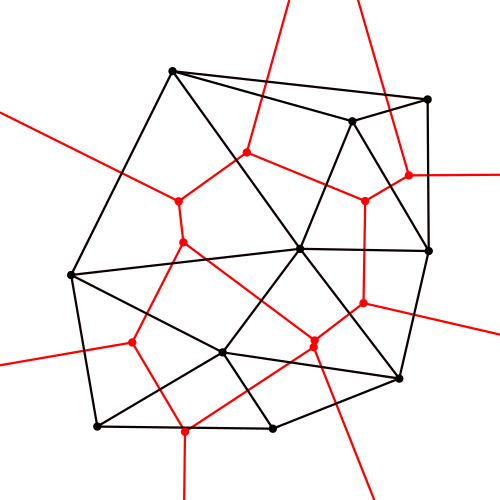
\includegraphics[width=\paperwidth,trim=-36mm -28mm -34mm 0]{figures/algorithms}}}% Insert image
\renewcommand{\parthook}{}}% Restore \parthook
\part{\done Algorithms}
\chapter{Decision Trees for $k$-SUM}
\label{chapter:ksum-algorithm}

Given three sets of \(n\) real numbers
\(A = \{\, a_1 < a_2 < \cdots < a_n\,\} \),
\(B = \{\, b_1 < b_2 < \cdots < b_n\,\} \),
and \(C = \{\, c_1 < c_2 < \cdots < c_n\,\}\),
we wish to build a discrete data structure (using bits, words, and pointers) such that,
given any triple \((i,j,k) \in {[n]}^3\) it is possible to compute the sign of
\(a_i + b_j + c_k\) by only inspecting the data structure (we cannot consult
\(A\), \(B\), or \(C\)).
We refer to the map $\chi : {[n]}^3\to \{-,0,+\}, (i,j,k)\mapsto\mathrm{sgn}
(a_i+b_i+c_k)$ as the {\em 3SUM-type} of the instance $\langle A,B,C \rangle$.
Obviously, one can simply construct a lookup table of size \(O(n^3)\), such
that triple queries can be answered in \(O(1)\) time. We aim at improving on
this trivial solution.

In the 3SUM problem, we are given an array of numbers as input and are asked
whether any three of them sum to 0. In the mid-nineties, this problem was
identified as a bottleneck of many
important problems in geometry, such as detection of affine degeneracies or
motion planning~\cite{GO95}. Since then, it has become a central problem in
fine-grained complexity theory~\cite{PW10}. It has long been conjectured to
require $\Omega (n^2)$ time. In 2014, it was shown to be solvable in $o(n^2)$
time, but no algorithm with running time $O(n^{2-\delta})$ with constant
$\delta>0$ is known~\cite{GP18}.

Lower bounds exist in restricted models of computation. Most notably,
$\Omega(n^2)$ 3-linear queries are needed to solve 3SUM~\cite{Er99a},
and nontrivial lower bounds have also been proven for slightly more powerful linear
decision trees~\cite{AC05}. However, in a recent breakthrough contribution, Kane, Lovett,
and Moran showed that 3SUM could be solved using $O(n\log^2 n)$
6-linear queries~\cite{KLM18}, hence within a $O(\log n)$ factor of the
information-theoretic lower bound.

Linear decision trees are examples of {\em nonuniform algorithms}, in which we
are allowed to have different algorithms for different input sizes.
Algebraic decision trees generalize linear decision trees
by allowing decision based on the sign of constant-degree polynomials at each
node~\cite{SY82}.

Any decision tree identifying the 3SUM-type of a 3SUM instance yields a concise
encoding of this 3SUM-type:
just write down the outcome of the successive tests. Knowing the decision tree
by convention, this sequence of bits is
sufficient to recover the sign of any triple.

The question we consider here is how to make such a representation efficient,
in the sense that not only does it use merely a few bits, but the answer to any
triple query can be recovered efficiently. Understanding the interplay between
nonuniform algorithms and such data structures hopefully sheds light on the
intrinsic structure of the problem.

\paragraph{Contribution}

As there are only $O(n^3)$ queries, a table
of size $(\log_2 3) n^3 + O(1)$ bits suffices to give constant query time
\cite{DPT10}. This can be improved to $O(n^2\log n)$ bits of space by
storing for each pair $(i,j)$ the values
\(k_<(i,j) = \max \{ 0\}\cup \{k \colon\, a_i + b_j + c_k < 0\}\) and
\(k_>(i,j) = \min \{ N+1\}\cup \{k \colon\, a_i + b_j + c_k > 0\}\).
For a query \((i,j,k)\), we compare \(k\) against the values \(k_<(i,j)\) and \(k_>(i,j)\)
to recover \(\chi(i,j,k)\) in \(O(1)\) time. All \(k_<(i,j)\) and \(k_>(i,j)\)
can be computed in \(O(n^2)\) time via the classic quadratic time algorithm for
3SUM.
%: if \(k \leq k_<(i,j)\), then \(\chi(i,j,k)=-1\), if \( k_<(i,j)< k < k_>(i,j)\),
%then \(\chi(i,j,k)=0\), and if \( k_>(i,j)\leq k\), then \(\chi(i,j,k)=+1\).
%The representation takes \( O(n^2 \log N \) bits, and each query can be answered by comparing
%pairs of indices, which takes \(O(1)\) time.

One seemingly simple representation is to store the numbers in $A$, $B$ and
$C$; however these are reals and thus we need to make them representable using
a finite number of bits.
In \S\ref{s:numbers} we show that a minimal integer representation of a
3SUM instance may require $\Theta(n)$ bits per value, which would give
rise to a $O(n)$ query time and $O(n^2)$ space, which is far from
impressive.
In \cite{CCILO18} the problem of given a set of $N$ lines, to create an
encoding of them so that the orientation of any triple (the \emph{order type})
can be determined was studied; our problem is a special case of this where the
lines only have three slopes.
Can we do better for the case of 3SUM? We answer this in the affirmative.
In \S\ref{s:space} we show how to use an optimal $O(n \log n)$ bits of
space with a polynomial query time. Finally, in section~\ref{s:sscqt} we show
how to use $\tilde{O}(n^{3/2})$ space to achieve $O(1)$-time queries.

\section{Sorting}

QUOTE ``Please, pretty please, order those data from smallest to largest''.

The sorting problem is one of the oldest and most practical data management
problems.
%
Usually, sorting is about permutations in \emph{arrays}, but we do not like
that. We use a different abstraction:

\input{text/definition/sorting}

Without any

\subsection{Algorithms}
Explain models of computation: uniform nonuniform etc

\subsection{Data Structures}

Most (if not all) algorithms for sorting receive their input data as a list and
output their answer as a permutation of this data. This permutation is a
compact data structure: the structure takes space proportional to the minimum
amount of space possible (about \(\log_2 n!\)), and the answer to each
comparison can be retrieved instantly from the structure.


\section{The \(k\)-SUM Problem}

The \(k\)-SUM problem is simple enough: given a list of \(n\) real numbers,
decide whether \(k\) of them sum to zero.

\input{text/definition/ksum}

For fixed \(k\), the \(k\)-SUM problem can be solved in polynomial time
\(O(n^k)\) by testing all possible candidate solutions.
The interesting question is whether it is possible to improve on
this brute-force solution.

The \(k\)-SUM problem is defined as follows: given a collection of $n$ real
numbers decide whether any $k$ of them sum to zero, where $k$ is a constant.
It is a fixed-parameter version of the subset-sum problem, a standard \textit{NP}-complete
problem. The \(k\)-SUM problem, and in particular the special case of 3SUM,
has proved to be a cornerstone of the fine-grained complexity program aiming at
the construction of a complexity theory for problems in $P$. In particular,
there are deep connections between the complexity of \(k\)-SUM, the Strong
Exponential Time Hypothesis~\cite{PW10,CGIMPS15}, and the complexity of many
other major problems in
$P$~\cite{GO95,BH99,MO01,P10,ACLL14,AVW14,GP14,KPP14,ALW14,AWY15,CL15}.

It has been long known that the \(k\)-SUM problem can be solved in time
$O(n^{\frac{k}{2}}\log n)$ for even $k$, and $O(n^{\frac{k+1}{2}})$ for odd
$k$. Erickson~\cite{Er99} proved a near-matching lower bound in the $k$-linear
decision tree model. In this model, the complexity is measured by the depth of
a decision tree, every node of which corresponds to a query of the form
$q_{i_1} + q_{i_2} + \cdots + q_{i_k} \ask{\le} 0$, where $q_1, q_2, \ldots, q_n$ are the
input numbers. In a recent breakthrough paper, Gr\o nlund and
Pettie~\cite{GP14} showed that in the $(2k-2)$-linear decision tree model,
where queries test the sign of weighted sums of up to $2k-2$ input numbers, only
$O(n^\frac{k}{2}\sqrt{\log n})$ queries are required for odd values of $k$. In
particular, there exists a $4$-linear decision tree for 3SUM of depth
$\tilde{O}(n^\frac{3}{2})$ (here the notation $\tilde{O}$ ignores polylogarithmic
factors), while every 3-linear decision tree has depth $\Omega
(n^2)$~\cite{Er99}. This indicates that increasing the size of the queries,
defined as the maximum number of input numbers involved in a query, can yield
significant improvements on the depth of the minimal-height decision tree. Ailon and
Chazelle~\cite{AC05} slightly extended the range of query sizes for which a
nontrivial lower bound could be established, elaborating on Erickson's
technique.

It has been well established that there exist nonuniform
polynomial-time algorithms for the subset-sum problem. One of them was
described by Meiser~\cite{M93}, and is derived from a data structure for point
location in arrangements of hyperplanes using the bottom vertex decomposition.
This algorithm can be cast as the construction of a linear decision tree in which
the queries have non-constant size.

\subsection{Our results}
In Section~\ref{sec:query-complexity}, we show the existence of an $n$-linear
decision tree of depth $\tilde{O}(n^3)$ for \(k\)-SUM using a careful
implementation of Meiser's algorithm~\cite{M93}.
Although the high-level algorithm itself is not new, we refine the
implementation and analysis for the \(k\)-SUM problem.%
\footnote{After submitting this manuscript, we learned from a personal communication
with Herv\'e Fournier that a similar analysis for arbitrary hyperplanes appears in his PhD
thesis~\cite{F01} (in French).}
Meiser presented his algorithm as a general method of point location in $m$
given $n$-dimensional hyperplanes that yielded a $\tilde{O}(n^4 \log
m)$-depth algebraic computation tree; when viewing the \(k\)-SUM problem as a point
location problem, $m$ is $O(n^k)$ and thus Meiser's algorithm can be viewed
as giving a $\tilde{O}(n^4)$-depth algebraic computation tree.
We show that while the
original algorithm was cast as a nonuniform polynomial-time algorithm,
it can be implemented in the linear decision tree model with an
$\tilde{O}(n^3)$ upper bound.
Moreover, this result implies the same improved upper bound on the depth of
algebraic computation trees for the $k$-SUM problem,
as shown in Appendix~\ref{app:act}.

There are two subtleties to this result. The first is inherent to the chosen
complexity model: even if the number of queries to the input is small (in
particular, the degree of the polynomial complexity is invariant on $k$), the
time required to \emph{determine which queries should be performed} may be
arbitrary. In a na\"ive analysis, we show it can be trivially bounded by
$\tilde{O}(n^{k+2})$. In Section~\ref{sec:time-complexity} we present an algorithm to
choose
which decisions to perform whereby the running time can be reduced to
$\tilde{O}(n^{\frac{k}{2}+8})$. Hence, we obtain an
$\tilde{O}(n^{\frac{k}{2}+8})$ time randomized algorithm in the RAM model
expected to perform $\tilde{O}(n^3)$ linear queries on the input\footnote{%
	Gr{\o}nlund and
	Pettie~\cite{GP14} mention the algorithms of Meyer auf der Heyde~\cite{M84} and
	Meiser~\cite{M93}, and state ``(\ldots) it was known that all \(k\)-LDT problems
	can be solved by $n$-linear decision trees with depth $O(n^5\log
	n)$~\cite{M93}, or with depth $O(n^4\log (nK))$ if the coefficients of the
	linear function are integers with absolute value at most $K$~\cite{M84}.
	Unfortunately these decision trees are not efficiently constructible. The
	time required to determine \emph{which} comparisons to make is
	exponential.'' We prove that the trees can have depth $\tilde{O}(n^3)$ and
	that the whole algorithm can run in randomized polynomial-time.}.

The second issue we address is that the linear queries in the above algorithm may
have size $n$, that is, they may use all the components of the input.
The lower bound of Erickson shows that if the queries are of minimal size, the number
of queries cannot be a polynomial independent of $k$ such as what we obtain, so
non-minimal query size is clearly essential to a drastic reduction in the number of queries needed.
This gives rise to the natural question as to what is the relation between query size and number of queries.
In particular, one natural question is whether queries of size less than $n$
would still allow the problem to be solved using a number of queries that is a
polynomial independent of $k$. We show that this is possible; in Section~\ref{sec:query-size},
we introduce a range of
algorithms exhibiting an explicit tradeoff between the number of queries and
their size. Using a blocking scheme, we show that we can restrict to
$o(n)$-linear decision trees. We also give a
range of tradeoffs for $O(n^{1-\alpha})$-linear decision trees. Although the
proposed algorithms still involve nonconstant-size queries, this is
the first time such tradeoffs are explicitly tackled. Table~\ref{tab:results} summarizes our results.

\begin{table}
\centering
\caption{Complexities of our new algorithms for the \(k\)-SUM problem. The query
size is the maximum number of elements of the input that can be involved in a
single linear query. The number of blocks is a parameter that allows us to
change the query size (see Section~\ref{sec:query-size}).
The origin of the constant in the exponent of the time complexity is due to
Lemma~\ref{lem:bound}. We conjecture it can be reduced, though substantial
changes in the analysis will likely be needed to do so.}
\label{tab:results}
\begin{tabular}{|c|c|c|c|c|}
	\hline

	& \# blocks & query size & \# queries & time \\
	\hline
	Theorem~\ref{thm:cube} &
	$1$ &
	$n$ &
	$\tilde{O}(n^3)$ & $\tilde{O}(n^{\lceil\frac{k}{2}}+8\rceil)$
	\\

	\hline

	Theorem~\ref{thm:query-size} &
	$b$ &
	$k\lceil\frac{n}{b}\rceil$ &
	$\tilde{O}(b^{k-4}n^3)$ &
	$\tilde{O}(b^{\lfloor\frac{k}{2}}-9\rfloor n^{\lceil\frac{k}{2}}+8\rceil)$
	\\

	\hline

	Corollary~\ref{cor:logn} &
	$b=\Theta(\polylog(n))$ &
	$o(n)$ &
	$\tilde{O}(n^3)$ &
	$\tilde{O}(n^{\lceil\frac{k}{2}}+8\rceil)$
	\\

	\hline

	Corollary~\ref{cor:ne} &
	$b=\Theta(n^\alpha)$ &
	$O(n^{1-\alpha})$ &
	$\tilde{O}(n^{3+(k-4)\alpha})$ &
	$\tilde{O}(n^{(1+\alpha)\frac{k}{2} +8.5})$
	\\

	\hline
\end{tabular}
\end{table}

\section{The Geometric View}

\chapter{Recent Breakthrough}

\section{It is always easier in the plane}

\input{text/paper/order-type-encoding/text/section/03-lines-and-pseudolines}
\input{text/paper/order-type-encoding/text/section/04-improve-query-complexity}

%\section{Higher-Dimensional Encodings}\label{sec:hyperplanes}
\section{Encoding Chirotopes of Hyperplane Arrangements}\label{sec:hyperplanes}

\input{text/paper/order-type-encoding/text/section/05-hyperplanes}

\section{Even Better Nonuniform Algorithms}

\subsection{Using Vertical Decomposition}

Ezra and
Sharir~\cite{ES17}
later improved the decision tree depth to \( O(n^2 \log n) \) by using
vertical decomposition instead.

\subsection{Inference Dimension}

In a breakthrough result, Kane, Lovett, and Moran~\cite{KLM18} proved
that $k$-SUM can be solved using $O(n \log^2 n)$ $2k$-linear queries. This is
close to the information theoretic lower bound of $\Omega(n \log n)$. Their
decision tree is also a prune and search algorithm.

\section{Open Questions}

Better uniform algorithms for 3SUM and 3POL.

Better nonuniform lower bound for 3SUM with 4-linear queries.

Nonuniform algorithm for 3POL based on inference dimension.

GPT in subquadratic time.


\chapter{Decision Trees for $k$-SUM}
\label{chapter:ksum-algorithm}

Given three sets of \(n\) real numbers
\(A = \{\, a_1 < a_2 < \cdots < a_n\,\} \),
\(B = \{\, b_1 < b_2 < \cdots < b_n\,\} \),
and \(C = \{\, c_1 < c_2 < \cdots < c_n\,\}\),
we wish to build a discrete data structure (using bits, words, and pointers) such that,
given any triple \((i,j,k) \in {[n]}^3\) it is possible to compute the sign of
\(a_i + b_j + c_k\) by only inspecting the data structure (we cannot consult
\(A\), \(B\), or \(C\)).
We refer to the map $\chi : {[n]}^3\to \{-,0,+\}, (i,j,k)\mapsto\mathrm{sgn}
(a_i+b_i+c_k)$ as the {\em 3SUM-type} of the instance $\langle A,B,C \rangle$.
Obviously, one can simply construct a lookup table of size \(O(n^3)\), such
that triple queries can be answered in \(O(1)\) time. We aim at improving on
this trivial solution.

In the 3SUM problem, we are given an array of numbers as input and are asked
whether any three of them sum to 0. In the mid-nineties, this problem was
identified as a bottleneck of many
important problems in geometry, such as detection of affine degeneracies or
motion planning~\cite{GO95}. Since then, it has become a central problem in
fine-grained complexity theory~\cite{PW10}. It has long been conjectured to
require $\Omega (n^2)$ time. In 2014, it was shown to be solvable in $o(n^2)$
time, but no algorithm with running time $O(n^{2-\delta})$ with constant
$\delta>0$ is known~\cite{GP18}.

Lower bounds exist in restricted models of computation. Most notably,
$\Omega(n^2)$ 3-linear queries are needed to solve 3SUM~\cite{Er99a},
and nontrivial lower bounds have also been proven for slightly more powerful linear
decision trees~\cite{AC05}. However, in a recent breakthrough contribution, Kane, Lovett,
and Moran showed that 3SUM could be solved using $O(n\log^2 n)$
6-linear queries~\cite{KLM18}, hence within a $O(\log n)$ factor of the
information-theoretic lower bound.

Linear decision trees are examples of {\em nonuniform algorithms}, in which we
are allowed to have different algorithms for different input sizes.
Algebraic decision trees generalize linear decision trees
by allowing decision based on the sign of constant-degree polynomials at each
node~\cite{SY82}.

Any decision tree identifying the 3SUM-type of a 3SUM instance yields a concise
encoding of this 3SUM-type:
just write down the outcome of the successive tests. Knowing the decision tree
by convention, this sequence of bits is
sufficient to recover the sign of any triple.

The question we consider here is how to make such a representation efficient,
in the sense that not only does it use merely a few bits, but the answer to any
triple query can be recovered efficiently. Understanding the interplay between
nonuniform algorithms and such data structures hopefully sheds light on the
intrinsic structure of the problem.

\paragraph{Contribution}

As there are only $O(n^3)$ queries, a table
of size $(\log_2 3) n^3 + O(1)$ bits suffices to give constant query time
\cite{DPT10}. This can be improved to $O(n^2\log n)$ bits of space by
storing for each pair $(i,j)$ the values
\(k_<(i,j) = \max \{ 0\}\cup \{k \colon\, a_i + b_j + c_k < 0\}\) and
\(k_>(i,j) = \min \{ N+1\}\cup \{k \colon\, a_i + b_j + c_k > 0\}\).
For a query \((i,j,k)\), we compare \(k\) against the values \(k_<(i,j)\) and \(k_>(i,j)\)
to recover \(\chi(i,j,k)\) in \(O(1)\) time. All \(k_<(i,j)\) and \(k_>(i,j)\)
can be computed in \(O(n^2)\) time via the classic quadratic time algorithm for
3SUM.
%: if \(k \leq k_<(i,j)\), then \(\chi(i,j,k)=-1\), if \( k_<(i,j)< k < k_>(i,j)\),
%then \(\chi(i,j,k)=0\), and if \( k_>(i,j)\leq k\), then \(\chi(i,j,k)=+1\).
%The representation takes \( O(n^2 \log N \) bits, and each query can be answered by comparing
%pairs of indices, which takes \(O(1)\) time.

One seemingly simple representation is to store the numbers in $A$, $B$ and
$C$; however these are reals and thus we need to make them representable using
a finite number of bits.
In \S\ref{s:numbers} we show that a minimal integer representation of a
3SUM instance may require $\Theta(n)$ bits per value, which would give
rise to a $O(n)$ query time and $O(n^2)$ space, which is far from
impressive.
In \cite{CCILO18} the problem of given a set of $N$ lines, to create an
encoding of them so that the orientation of any triple (the \emph{order type})
can be determined was studied; our problem is a special case of this where the
lines only have three slopes.
Can we do better for the case of 3SUM? We answer this in the affirmative.
In \S\ref{s:space} we show how to use an optimal $O(n \log n)$ bits of
space with a polynomial query time. Finally, in section~\ref{s:sscqt} we show
how to use $\tilde{O}(n^{3/2})$ space to achieve $O(1)$-time queries.

\section{Sorting}

QUOTE ``Please, pretty please, order those data from smallest to largest''.

The sorting problem is one of the oldest and most practical data management
problems.
%
Usually, sorting is about permutations in \emph{arrays}, but we do not like
that. We use a different abstraction:

\input{text/definition/sorting}

Without any

\subsection{Algorithms}
Explain models of computation: uniform nonuniform etc

\subsection{Data Structures}

Most (if not all) algorithms for sorting receive their input data as a list and
output their answer as a permutation of this data. This permutation is a
compact data structure: the structure takes space proportional to the minimum
amount of space possible (about \(\log_2 n!\)), and the answer to each
comparison can be retrieved instantly from the structure.


\section{The \(k\)-SUM Problem}

The \(k\)-SUM problem is simple enough: given a list of \(n\) real numbers,
decide whether \(k\) of them sum to zero.

\input{text/definition/ksum}

For fixed \(k\), the \(k\)-SUM problem can be solved in polynomial time
\(O(n^k)\) by testing all possible candidate solutions.
The interesting question is whether it is possible to improve on
this brute-force solution.

The \(k\)-SUM problem is defined as follows: given a collection of $n$ real
numbers decide whether any $k$ of them sum to zero, where $k$ is a constant.
It is a fixed-parameter version of the subset-sum problem, a standard \textit{NP}-complete
problem. The \(k\)-SUM problem, and in particular the special case of 3SUM,
has proved to be a cornerstone of the fine-grained complexity program aiming at
the construction of a complexity theory for problems in $P$. In particular,
there are deep connections between the complexity of \(k\)-SUM, the Strong
Exponential Time Hypothesis~\cite{PW10,CGIMPS15}, and the complexity of many
other major problems in
$P$~\cite{GO95,BH99,MO01,P10,ACLL14,AVW14,GP14,KPP14,ALW14,AWY15,CL15}.

It has been long known that the \(k\)-SUM problem can be solved in time
$O(n^{\frac{k}{2}}\log n)$ for even $k$, and $O(n^{\frac{k+1}{2}})$ for odd
$k$. Erickson~\cite{Er99} proved a near-matching lower bound in the $k$-linear
decision tree model. In this model, the complexity is measured by the depth of
a decision tree, every node of which corresponds to a query of the form
$q_{i_1} + q_{i_2} + \cdots + q_{i_k} \ask{\le} 0$, where $q_1, q_2, \ldots, q_n$ are the
input numbers. In a recent breakthrough paper, Gr\o nlund and
Pettie~\cite{GP14} showed that in the $(2k-2)$-linear decision tree model,
where queries test the sign of weighted sums of up to $2k-2$ input numbers, only
$O(n^\frac{k}{2}\sqrt{\log n})$ queries are required for odd values of $k$. In
particular, there exists a $4$-linear decision tree for 3SUM of depth
$\tilde{O}(n^\frac{3}{2})$ (here the notation $\tilde{O}$ ignores polylogarithmic
factors), while every 3-linear decision tree has depth $\Omega
(n^2)$~\cite{Er99}. This indicates that increasing the size of the queries,
defined as the maximum number of input numbers involved in a query, can yield
significant improvements on the depth of the minimal-height decision tree. Ailon and
Chazelle~\cite{AC05} slightly extended the range of query sizes for which a
nontrivial lower bound could be established, elaborating on Erickson's
technique.

It has been well established that there exist nonuniform
polynomial-time algorithms for the subset-sum problem. One of them was
described by Meiser~\cite{M93}, and is derived from a data structure for point
location in arrangements of hyperplanes using the bottom vertex decomposition.
This algorithm can be cast as the construction of a linear decision tree in which
the queries have non-constant size.

\subsection{Our results}
In Section~\ref{sec:query-complexity}, we show the existence of an $n$-linear
decision tree of depth $\tilde{O}(n^3)$ for \(k\)-SUM using a careful
implementation of Meiser's algorithm~\cite{M93}.
Although the high-level algorithm itself is not new, we refine the
implementation and analysis for the \(k\)-SUM problem.%
\footnote{After submitting this manuscript, we learned from a personal communication
with Herv\'e Fournier that a similar analysis for arbitrary hyperplanes appears in his PhD
thesis~\cite{F01} (in French).}
Meiser presented his algorithm as a general method of point location in $m$
given $n$-dimensional hyperplanes that yielded a $\tilde{O}(n^4 \log
m)$-depth algebraic computation tree; when viewing the \(k\)-SUM problem as a point
location problem, $m$ is $O(n^k)$ and thus Meiser's algorithm can be viewed
as giving a $\tilde{O}(n^4)$-depth algebraic computation tree.
We show that while the
original algorithm was cast as a nonuniform polynomial-time algorithm,
it can be implemented in the linear decision tree model with an
$\tilde{O}(n^3)$ upper bound.
Moreover, this result implies the same improved upper bound on the depth of
algebraic computation trees for the $k$-SUM problem,
as shown in Appendix~\ref{app:act}.

There are two subtleties to this result. The first is inherent to the chosen
complexity model: even if the number of queries to the input is small (in
particular, the degree of the polynomial complexity is invariant on $k$), the
time required to \emph{determine which queries should be performed} may be
arbitrary. In a na\"ive analysis, we show it can be trivially bounded by
$\tilde{O}(n^{k+2})$. In Section~\ref{sec:time-complexity} we present an algorithm to
choose
which decisions to perform whereby the running time can be reduced to
$\tilde{O}(n^{\frac{k}{2}+8})$. Hence, we obtain an
$\tilde{O}(n^{\frac{k}{2}+8})$ time randomized algorithm in the RAM model
expected to perform $\tilde{O}(n^3)$ linear queries on the input\footnote{%
	Gr{\o}nlund and
	Pettie~\cite{GP14} mention the algorithms of Meyer auf der Heyde~\cite{M84} and
	Meiser~\cite{M93}, and state ``(\ldots) it was known that all \(k\)-LDT problems
	can be solved by $n$-linear decision trees with depth $O(n^5\log
	n)$~\cite{M93}, or with depth $O(n^4\log (nK))$ if the coefficients of the
	linear function are integers with absolute value at most $K$~\cite{M84}.
	Unfortunately these decision trees are not efficiently constructible. The
	time required to determine \emph{which} comparisons to make is
	exponential.'' We prove that the trees can have depth $\tilde{O}(n^3)$ and
	that the whole algorithm can run in randomized polynomial-time.}.

The second issue we address is that the linear queries in the above algorithm may
have size $n$, that is, they may use all the components of the input.
The lower bound of Erickson shows that if the queries are of minimal size, the number
of queries cannot be a polynomial independent of $k$ such as what we obtain, so
non-minimal query size is clearly essential to a drastic reduction in the number of queries needed.
This gives rise to the natural question as to what is the relation between query size and number of queries.
In particular, one natural question is whether queries of size less than $n$
would still allow the problem to be solved using a number of queries that is a
polynomial independent of $k$. We show that this is possible; in Section~\ref{sec:query-size},
we introduce a range of
algorithms exhibiting an explicit tradeoff between the number of queries and
their size. Using a blocking scheme, we show that we can restrict to
$o(n)$-linear decision trees. We also give a
range of tradeoffs for $O(n^{1-\alpha})$-linear decision trees. Although the
proposed algorithms still involve nonconstant-size queries, this is
the first time such tradeoffs are explicitly tackled. Table~\ref{tab:results} summarizes our results.

\begin{table}
\centering
\caption{Complexities of our new algorithms for the \(k\)-SUM problem. The query
size is the maximum number of elements of the input that can be involved in a
single linear query. The number of blocks is a parameter that allows us to
change the query size (see Section~\ref{sec:query-size}).
The origin of the constant in the exponent of the time complexity is due to
Lemma~\ref{lem:bound}. We conjecture it can be reduced, though substantial
changes in the analysis will likely be needed to do so.}
\label{tab:results}
\begin{tabular}{|c|c|c|c|c|}
	\hline

	& \# blocks & query size & \# queries & time \\
	\hline
	Theorem~\ref{thm:cube} &
	$1$ &
	$n$ &
	$\tilde{O}(n^3)$ & $\tilde{O}(n^{\lceil\frac{k}{2}}+8\rceil)$
	\\

	\hline

	Theorem~\ref{thm:query-size} &
	$b$ &
	$k\lceil\frac{n}{b}\rceil$ &
	$\tilde{O}(b^{k-4}n^3)$ &
	$\tilde{O}(b^{\lfloor\frac{k}{2}}-9\rfloor n^{\lceil\frac{k}{2}}+8\rceil)$
	\\

	\hline

	Corollary~\ref{cor:logn} &
	$b=\Theta(\polylog(n))$ &
	$o(n)$ &
	$\tilde{O}(n^3)$ &
	$\tilde{O}(n^{\lceil\frac{k}{2}}+8\rceil)$
	\\

	\hline

	Corollary~\ref{cor:ne} &
	$b=\Theta(n^\alpha)$ &
	$O(n^{1-\alpha})$ &
	$\tilde{O}(n^{3+(k-4)\alpha})$ &
	$\tilde{O}(n^{(1+\alpha)\frac{k}{2} +8.5})$
	\\

	\hline
\end{tabular}
\end{table}

\section{The Geometric View}

\chapter{Recent Breakthrough}

\section{It is always easier in the plane}

\input{text/paper/order-type-encoding/text/section/03-lines-and-pseudolines}
\input{text/paper/order-type-encoding/text/section/04-improve-query-complexity}

%\section{Higher-Dimensional Encodings}\label{sec:hyperplanes}
\section{Encoding Chirotopes of Hyperplane Arrangements}\label{sec:hyperplanes}

\input{text/paper/order-type-encoding/text/section/05-hyperplanes}

\section{Even Better Nonuniform Algorithms}

\subsection{Using Vertical Decomposition}

Ezra and
Sharir~\cite{ES17}
later improved the decision tree depth to \( O(n^2 \log n) \) by using
vertical decomposition instead.

\subsection{Inference Dimension}

In a breakthrough result, Kane, Lovett, and Moran~\cite{KLM18} proved
that $k$-SUM can be solved using $O(n \log^2 n)$ $2k$-linear queries. This is
close to the information theoretic lower bound of $\Omega(n \log n)$. Their
decision tree is also a prune and search algorithm.

\section{Open Questions}

Better uniform algorithms for 3SUM and 3POL.

Better nonuniform lower bound for 3SUM with 4-linear queries.

Nonuniform algorithm for 3POL based on inference dimension.

GPT in subquadratic time.



\clearemptydoublepage
\renewcommand{\parthook}{% Update \parthook
\AddToShipoutPictureBG*{% Add picture to background of THIS page only
\AtPageLowerLeft{\includegraphics[width=\paperwidth,trim=-36mm -33mm -34mm 0]{figures/data-structures}}}% Insert image
%\AtPageLowerLeft{\centerline{\includegraphics[height=10cm,trim=0 -28mm 0 0]{figures/data-structures}}}}% Insert image
\renewcommand{\parthook}{}}% Restore \parthook
\part{\done Data Structures}
\chapter{Decision Trees for $k$-SUM}
\label{chapter:ksum-algorithm}

Given three sets of \(n\) real numbers
\(A = \{\, a_1 < a_2 < \cdots < a_n\,\} \),
\(B = \{\, b_1 < b_2 < \cdots < b_n\,\} \),
and \(C = \{\, c_1 < c_2 < \cdots < c_n\,\}\),
we wish to build a discrete data structure (using bits, words, and pointers) such that,
given any triple \((i,j,k) \in {[n]}^3\) it is possible to compute the sign of
\(a_i + b_j + c_k\) by only inspecting the data structure (we cannot consult
\(A\), \(B\), or \(C\)).
We refer to the map $\chi : {[n]}^3\to \{-,0,+\}, (i,j,k)\mapsto\mathrm{sgn}
(a_i+b_i+c_k)$ as the {\em 3SUM-type} of the instance $\langle A,B,C \rangle$.
Obviously, one can simply construct a lookup table of size \(O(n^3)\), such
that triple queries can be answered in \(O(1)\) time. We aim at improving on
this trivial solution.

In the 3SUM problem, we are given an array of numbers as input and are asked
whether any three of them sum to 0. In the mid-nineties, this problem was
identified as a bottleneck of many
important problems in geometry, such as detection of affine degeneracies or
motion planning~\cite{GO95}. Since then, it has become a central problem in
fine-grained complexity theory~\cite{PW10}. It has long been conjectured to
require $\Omega (n^2)$ time. In 2014, it was shown to be solvable in $o(n^2)$
time, but no algorithm with running time $O(n^{2-\delta})$ with constant
$\delta>0$ is known~\cite{GP18}.

Lower bounds exist in restricted models of computation. Most notably,
$\Omega(n^2)$ 3-linear queries are needed to solve 3SUM~\cite{Er99a},
and nontrivial lower bounds have also been proven for slightly more powerful linear
decision trees~\cite{AC05}. However, in a recent breakthrough contribution, Kane, Lovett,
and Moran showed that 3SUM could be solved using $O(n\log^2 n)$
6-linear queries~\cite{KLM18}, hence within a $O(\log n)$ factor of the
information-theoretic lower bound.

Linear decision trees are examples of {\em nonuniform algorithms}, in which we
are allowed to have different algorithms for different input sizes.
Algebraic decision trees generalize linear decision trees
by allowing decision based on the sign of constant-degree polynomials at each
node~\cite{SY82}.

Any decision tree identifying the 3SUM-type of a 3SUM instance yields a concise
encoding of this 3SUM-type:
just write down the outcome of the successive tests. Knowing the decision tree
by convention, this sequence of bits is
sufficient to recover the sign of any triple.

The question we consider here is how to make such a representation efficient,
in the sense that not only does it use merely a few bits, but the answer to any
triple query can be recovered efficiently. Understanding the interplay between
nonuniform algorithms and such data structures hopefully sheds light on the
intrinsic structure of the problem.

\paragraph{Contribution}

As there are only $O(n^3)$ queries, a table
of size $(\log_2 3) n^3 + O(1)$ bits suffices to give constant query time
\cite{DPT10}. This can be improved to $O(n^2\log n)$ bits of space by
storing for each pair $(i,j)$ the values
\(k_<(i,j) = \max \{ 0\}\cup \{k \colon\, a_i + b_j + c_k < 0\}\) and
\(k_>(i,j) = \min \{ N+1\}\cup \{k \colon\, a_i + b_j + c_k > 0\}\).
For a query \((i,j,k)\), we compare \(k\) against the values \(k_<(i,j)\) and \(k_>(i,j)\)
to recover \(\chi(i,j,k)\) in \(O(1)\) time. All \(k_<(i,j)\) and \(k_>(i,j)\)
can be computed in \(O(n^2)\) time via the classic quadratic time algorithm for
3SUM.
%: if \(k \leq k_<(i,j)\), then \(\chi(i,j,k)=-1\), if \( k_<(i,j)< k < k_>(i,j)\),
%then \(\chi(i,j,k)=0\), and if \( k_>(i,j)\leq k\), then \(\chi(i,j,k)=+1\).
%The representation takes \( O(n^2 \log N \) bits, and each query can be answered by comparing
%pairs of indices, which takes \(O(1)\) time.

One seemingly simple representation is to store the numbers in $A$, $B$ and
$C$; however these are reals and thus we need to make them representable using
a finite number of bits.
In \S\ref{s:numbers} we show that a minimal integer representation of a
3SUM instance may require $\Theta(n)$ bits per value, which would give
rise to a $O(n)$ query time and $O(n^2)$ space, which is far from
impressive.
In \cite{CCILO18} the problem of given a set of $N$ lines, to create an
encoding of them so that the orientation of any triple (the \emph{order type})
can be determined was studied; our problem is a special case of this where the
lines only have three slopes.
Can we do better for the case of 3SUM? We answer this in the affirmative.
In \S\ref{s:space} we show how to use an optimal $O(n \log n)$ bits of
space with a polynomial query time. Finally, in section~\ref{s:sscqt} we show
how to use $\tilde{O}(n^{3/2})$ space to achieve $O(1)$-time queries.

\section{Sorting}

QUOTE ``Please, pretty please, order those data from smallest to largest''.

The sorting problem is one of the oldest and most practical data management
problems.
%
Usually, sorting is about permutations in \emph{arrays}, but we do not like
that. We use a different abstraction:

\input{text/definition/sorting}

Without any

\subsection{Algorithms}
Explain models of computation: uniform nonuniform etc

\subsection{Data Structures}

Most (if not all) algorithms for sorting receive their input data as a list and
output their answer as a permutation of this data. This permutation is a
compact data structure: the structure takes space proportional to the minimum
amount of space possible (about \(\log_2 n!\)), and the answer to each
comparison can be retrieved instantly from the structure.


\section{The \(k\)-SUM Problem}

The \(k\)-SUM problem is simple enough: given a list of \(n\) real numbers,
decide whether \(k\) of them sum to zero.

\input{text/definition/ksum}

For fixed \(k\), the \(k\)-SUM problem can be solved in polynomial time
\(O(n^k)\) by testing all possible candidate solutions.
The interesting question is whether it is possible to improve on
this brute-force solution.

The \(k\)-SUM problem is defined as follows: given a collection of $n$ real
numbers decide whether any $k$ of them sum to zero, where $k$ is a constant.
It is a fixed-parameter version of the subset-sum problem, a standard \textit{NP}-complete
problem. The \(k\)-SUM problem, and in particular the special case of 3SUM,
has proved to be a cornerstone of the fine-grained complexity program aiming at
the construction of a complexity theory for problems in $P$. In particular,
there are deep connections between the complexity of \(k\)-SUM, the Strong
Exponential Time Hypothesis~\cite{PW10,CGIMPS15}, and the complexity of many
other major problems in
$P$~\cite{GO95,BH99,MO01,P10,ACLL14,AVW14,GP14,KPP14,ALW14,AWY15,CL15}.

It has been long known that the \(k\)-SUM problem can be solved in time
$O(n^{\frac{k}{2}}\log n)$ for even $k$, and $O(n^{\frac{k+1}{2}})$ for odd
$k$. Erickson~\cite{Er99} proved a near-matching lower bound in the $k$-linear
decision tree model. In this model, the complexity is measured by the depth of
a decision tree, every node of which corresponds to a query of the form
$q_{i_1} + q_{i_2} + \cdots + q_{i_k} \ask{\le} 0$, where $q_1, q_2, \ldots, q_n$ are the
input numbers. In a recent breakthrough paper, Gr\o nlund and
Pettie~\cite{GP14} showed that in the $(2k-2)$-linear decision tree model,
where queries test the sign of weighted sums of up to $2k-2$ input numbers, only
$O(n^\frac{k}{2}\sqrt{\log n})$ queries are required for odd values of $k$. In
particular, there exists a $4$-linear decision tree for 3SUM of depth
$\tilde{O}(n^\frac{3}{2})$ (here the notation $\tilde{O}$ ignores polylogarithmic
factors), while every 3-linear decision tree has depth $\Omega
(n^2)$~\cite{Er99}. This indicates that increasing the size of the queries,
defined as the maximum number of input numbers involved in a query, can yield
significant improvements on the depth of the minimal-height decision tree. Ailon and
Chazelle~\cite{AC05} slightly extended the range of query sizes for which a
nontrivial lower bound could be established, elaborating on Erickson's
technique.

It has been well established that there exist nonuniform
polynomial-time algorithms for the subset-sum problem. One of them was
described by Meiser~\cite{M93}, and is derived from a data structure for point
location in arrangements of hyperplanes using the bottom vertex decomposition.
This algorithm can be cast as the construction of a linear decision tree in which
the queries have non-constant size.

\subsection{Our results}
In Section~\ref{sec:query-complexity}, we show the existence of an $n$-linear
decision tree of depth $\tilde{O}(n^3)$ for \(k\)-SUM using a careful
implementation of Meiser's algorithm~\cite{M93}.
Although the high-level algorithm itself is not new, we refine the
implementation and analysis for the \(k\)-SUM problem.%
\footnote{After submitting this manuscript, we learned from a personal communication
with Herv\'e Fournier that a similar analysis for arbitrary hyperplanes appears in his PhD
thesis~\cite{F01} (in French).}
Meiser presented his algorithm as a general method of point location in $m$
given $n$-dimensional hyperplanes that yielded a $\tilde{O}(n^4 \log
m)$-depth algebraic computation tree; when viewing the \(k\)-SUM problem as a point
location problem, $m$ is $O(n^k)$ and thus Meiser's algorithm can be viewed
as giving a $\tilde{O}(n^4)$-depth algebraic computation tree.
We show that while the
original algorithm was cast as a nonuniform polynomial-time algorithm,
it can be implemented in the linear decision tree model with an
$\tilde{O}(n^3)$ upper bound.
Moreover, this result implies the same improved upper bound on the depth of
algebraic computation trees for the $k$-SUM problem,
as shown in Appendix~\ref{app:act}.

There are two subtleties to this result. The first is inherent to the chosen
complexity model: even if the number of queries to the input is small (in
particular, the degree of the polynomial complexity is invariant on $k$), the
time required to \emph{determine which queries should be performed} may be
arbitrary. In a na\"ive analysis, we show it can be trivially bounded by
$\tilde{O}(n^{k+2})$. In Section~\ref{sec:time-complexity} we present an algorithm to
choose
which decisions to perform whereby the running time can be reduced to
$\tilde{O}(n^{\frac{k}{2}+8})$. Hence, we obtain an
$\tilde{O}(n^{\frac{k}{2}+8})$ time randomized algorithm in the RAM model
expected to perform $\tilde{O}(n^3)$ linear queries on the input\footnote{%
	Gr{\o}nlund and
	Pettie~\cite{GP14} mention the algorithms of Meyer auf der Heyde~\cite{M84} and
	Meiser~\cite{M93}, and state ``(\ldots) it was known that all \(k\)-LDT problems
	can be solved by $n$-linear decision trees with depth $O(n^5\log
	n)$~\cite{M93}, or with depth $O(n^4\log (nK))$ if the coefficients of the
	linear function are integers with absolute value at most $K$~\cite{M84}.
	Unfortunately these decision trees are not efficiently constructible. The
	time required to determine \emph{which} comparisons to make is
	exponential.'' We prove that the trees can have depth $\tilde{O}(n^3)$ and
	that the whole algorithm can run in randomized polynomial-time.}.

The second issue we address is that the linear queries in the above algorithm may
have size $n$, that is, they may use all the components of the input.
The lower bound of Erickson shows that if the queries are of minimal size, the number
of queries cannot be a polynomial independent of $k$ such as what we obtain, so
non-minimal query size is clearly essential to a drastic reduction in the number of queries needed.
This gives rise to the natural question as to what is the relation between query size and number of queries.
In particular, one natural question is whether queries of size less than $n$
would still allow the problem to be solved using a number of queries that is a
polynomial independent of $k$. We show that this is possible; in Section~\ref{sec:query-size},
we introduce a range of
algorithms exhibiting an explicit tradeoff between the number of queries and
their size. Using a blocking scheme, we show that we can restrict to
$o(n)$-linear decision trees. We also give a
range of tradeoffs for $O(n^{1-\alpha})$-linear decision trees. Although the
proposed algorithms still involve nonconstant-size queries, this is
the first time such tradeoffs are explicitly tackled. Table~\ref{tab:results} summarizes our results.

\begin{table}
\centering
\caption{Complexities of our new algorithms for the \(k\)-SUM problem. The query
size is the maximum number of elements of the input that can be involved in a
single linear query. The number of blocks is a parameter that allows us to
change the query size (see Section~\ref{sec:query-size}).
The origin of the constant in the exponent of the time complexity is due to
Lemma~\ref{lem:bound}. We conjecture it can be reduced, though substantial
changes in the analysis will likely be needed to do so.}
\label{tab:results}
\begin{tabular}{|c|c|c|c|c|}
	\hline

	& \# blocks & query size & \# queries & time \\
	\hline
	Theorem~\ref{thm:cube} &
	$1$ &
	$n$ &
	$\tilde{O}(n^3)$ & $\tilde{O}(n^{\lceil\frac{k}{2}}+8\rceil)$
	\\

	\hline

	Theorem~\ref{thm:query-size} &
	$b$ &
	$k\lceil\frac{n}{b}\rceil$ &
	$\tilde{O}(b^{k-4}n^3)$ &
	$\tilde{O}(b^{\lfloor\frac{k}{2}}-9\rfloor n^{\lceil\frac{k}{2}}+8\rceil)$
	\\

	\hline

	Corollary~\ref{cor:logn} &
	$b=\Theta(\polylog(n))$ &
	$o(n)$ &
	$\tilde{O}(n^3)$ &
	$\tilde{O}(n^{\lceil\frac{k}{2}}+8\rceil)$
	\\

	\hline

	Corollary~\ref{cor:ne} &
	$b=\Theta(n^\alpha)$ &
	$O(n^{1-\alpha})$ &
	$\tilde{O}(n^{3+(k-4)\alpha})$ &
	$\tilde{O}(n^{(1+\alpha)\frac{k}{2} +8.5})$
	\\

	\hline
\end{tabular}
\end{table}

\section{The Geometric View}

\chapter{Recent Breakthrough}

\section{It is always easier in the plane}

\input{text/paper/order-type-encoding/text/section/03-lines-and-pseudolines}
\input{text/paper/order-type-encoding/text/section/04-improve-query-complexity}

%\section{Higher-Dimensional Encodings}\label{sec:hyperplanes}
\section{Encoding Chirotopes of Hyperplane Arrangements}\label{sec:hyperplanes}

\input{text/paper/order-type-encoding/text/section/05-hyperplanes}

\section{Even Better Nonuniform Algorithms}

\subsection{Using Vertical Decomposition}

Ezra and
Sharir~\cite{ES17}
later improved the decision tree depth to \( O(n^2 \log n) \) by using
vertical decomposition instead.

\subsection{Inference Dimension}

In a breakthrough result, Kane, Lovett, and Moran~\cite{KLM18} proved
that $k$-SUM can be solved using $O(n \log^2 n)$ $2k$-linear queries. This is
close to the information theoretic lower bound of $\Omega(n \log n)$. Their
decision tree is also a prune and search algorithm.

\section{Open Questions}

Better uniform algorithms for 3SUM and 3POL.

Better nonuniform lower bound for 3SUM with 4-linear queries.

Nonuniform algorithm for 3POL based on inference dimension.

GPT in subquadratic time.


\chapter{Decision Trees for $k$-SUM}
\label{chapter:ksum-algorithm}

Given three sets of \(n\) real numbers
\(A = \{\, a_1 < a_2 < \cdots < a_n\,\} \),
\(B = \{\, b_1 < b_2 < \cdots < b_n\,\} \),
and \(C = \{\, c_1 < c_2 < \cdots < c_n\,\}\),
we wish to build a discrete data structure (using bits, words, and pointers) such that,
given any triple \((i,j,k) \in {[n]}^3\) it is possible to compute the sign of
\(a_i + b_j + c_k\) by only inspecting the data structure (we cannot consult
\(A\), \(B\), or \(C\)).
We refer to the map $\chi : {[n]}^3\to \{-,0,+\}, (i,j,k)\mapsto\mathrm{sgn}
(a_i+b_i+c_k)$ as the {\em 3SUM-type} of the instance $\langle A,B,C \rangle$.
Obviously, one can simply construct a lookup table of size \(O(n^3)\), such
that triple queries can be answered in \(O(1)\) time. We aim at improving on
this trivial solution.

In the 3SUM problem, we are given an array of numbers as input and are asked
whether any three of them sum to 0. In the mid-nineties, this problem was
identified as a bottleneck of many
important problems in geometry, such as detection of affine degeneracies or
motion planning~\cite{GO95}. Since then, it has become a central problem in
fine-grained complexity theory~\cite{PW10}. It has long been conjectured to
require $\Omega (n^2)$ time. In 2014, it was shown to be solvable in $o(n^2)$
time, but no algorithm with running time $O(n^{2-\delta})$ with constant
$\delta>0$ is known~\cite{GP18}.

Lower bounds exist in restricted models of computation. Most notably,
$\Omega(n^2)$ 3-linear queries are needed to solve 3SUM~\cite{Er99a},
and nontrivial lower bounds have also been proven for slightly more powerful linear
decision trees~\cite{AC05}. However, in a recent breakthrough contribution, Kane, Lovett,
and Moran showed that 3SUM could be solved using $O(n\log^2 n)$
6-linear queries~\cite{KLM18}, hence within a $O(\log n)$ factor of the
information-theoretic lower bound.

Linear decision trees are examples of {\em nonuniform algorithms}, in which we
are allowed to have different algorithms for different input sizes.
Algebraic decision trees generalize linear decision trees
by allowing decision based on the sign of constant-degree polynomials at each
node~\cite{SY82}.

Any decision tree identifying the 3SUM-type of a 3SUM instance yields a concise
encoding of this 3SUM-type:
just write down the outcome of the successive tests. Knowing the decision tree
by convention, this sequence of bits is
sufficient to recover the sign of any triple.

The question we consider here is how to make such a representation efficient,
in the sense that not only does it use merely a few bits, but the answer to any
triple query can be recovered efficiently. Understanding the interplay between
nonuniform algorithms and such data structures hopefully sheds light on the
intrinsic structure of the problem.

\paragraph{Contribution}

As there are only $O(n^3)$ queries, a table
of size $(\log_2 3) n^3 + O(1)$ bits suffices to give constant query time
\cite{DPT10}. This can be improved to $O(n^2\log n)$ bits of space by
storing for each pair $(i,j)$ the values
\(k_<(i,j) = \max \{ 0\}\cup \{k \colon\, a_i + b_j + c_k < 0\}\) and
\(k_>(i,j) = \min \{ N+1\}\cup \{k \colon\, a_i + b_j + c_k > 0\}\).
For a query \((i,j,k)\), we compare \(k\) against the values \(k_<(i,j)\) and \(k_>(i,j)\)
to recover \(\chi(i,j,k)\) in \(O(1)\) time. All \(k_<(i,j)\) and \(k_>(i,j)\)
can be computed in \(O(n^2)\) time via the classic quadratic time algorithm for
3SUM.
%: if \(k \leq k_<(i,j)\), then \(\chi(i,j,k)=-1\), if \( k_<(i,j)< k < k_>(i,j)\),
%then \(\chi(i,j,k)=0\), and if \( k_>(i,j)\leq k\), then \(\chi(i,j,k)=+1\).
%The representation takes \( O(n^2 \log N \) bits, and each query can be answered by comparing
%pairs of indices, which takes \(O(1)\) time.

One seemingly simple representation is to store the numbers in $A$, $B$ and
$C$; however these are reals and thus we need to make them representable using
a finite number of bits.
In \S\ref{s:numbers} we show that a minimal integer representation of a
3SUM instance may require $\Theta(n)$ bits per value, which would give
rise to a $O(n)$ query time and $O(n^2)$ space, which is far from
impressive.
In \cite{CCILO18} the problem of given a set of $N$ lines, to create an
encoding of them so that the orientation of any triple (the \emph{order type})
can be determined was studied; our problem is a special case of this where the
lines only have three slopes.
Can we do better for the case of 3SUM? We answer this in the affirmative.
In \S\ref{s:space} we show how to use an optimal $O(n \log n)$ bits of
space with a polynomial query time. Finally, in section~\ref{s:sscqt} we show
how to use $\tilde{O}(n^{3/2})$ space to achieve $O(1)$-time queries.

\section{Sorting}

QUOTE ``Please, pretty please, order those data from smallest to largest''.

The sorting problem is one of the oldest and most practical data management
problems.
%
Usually, sorting is about permutations in \emph{arrays}, but we do not like
that. We use a different abstraction:

\input{text/definition/sorting}

Without any

\subsection{Algorithms}
Explain models of computation: uniform nonuniform etc

\subsection{Data Structures}

Most (if not all) algorithms for sorting receive their input data as a list and
output their answer as a permutation of this data. This permutation is a
compact data structure: the structure takes space proportional to the minimum
amount of space possible (about \(\log_2 n!\)), and the answer to each
comparison can be retrieved instantly from the structure.


\section{The \(k\)-SUM Problem}

The \(k\)-SUM problem is simple enough: given a list of \(n\) real numbers,
decide whether \(k\) of them sum to zero.

\input{text/definition/ksum}

For fixed \(k\), the \(k\)-SUM problem can be solved in polynomial time
\(O(n^k)\) by testing all possible candidate solutions.
The interesting question is whether it is possible to improve on
this brute-force solution.

The \(k\)-SUM problem is defined as follows: given a collection of $n$ real
numbers decide whether any $k$ of them sum to zero, where $k$ is a constant.
It is a fixed-parameter version of the subset-sum problem, a standard \textit{NP}-complete
problem. The \(k\)-SUM problem, and in particular the special case of 3SUM,
has proved to be a cornerstone of the fine-grained complexity program aiming at
the construction of a complexity theory for problems in $P$. In particular,
there are deep connections between the complexity of \(k\)-SUM, the Strong
Exponential Time Hypothesis~\cite{PW10,CGIMPS15}, and the complexity of many
other major problems in
$P$~\cite{GO95,BH99,MO01,P10,ACLL14,AVW14,GP14,KPP14,ALW14,AWY15,CL15}.

It has been long known that the \(k\)-SUM problem can be solved in time
$O(n^{\frac{k}{2}}\log n)$ for even $k$, and $O(n^{\frac{k+1}{2}})$ for odd
$k$. Erickson~\cite{Er99} proved a near-matching lower bound in the $k$-linear
decision tree model. In this model, the complexity is measured by the depth of
a decision tree, every node of which corresponds to a query of the form
$q_{i_1} + q_{i_2} + \cdots + q_{i_k} \ask{\le} 0$, where $q_1, q_2, \ldots, q_n$ are the
input numbers. In a recent breakthrough paper, Gr\o nlund and
Pettie~\cite{GP14} showed that in the $(2k-2)$-linear decision tree model,
where queries test the sign of weighted sums of up to $2k-2$ input numbers, only
$O(n^\frac{k}{2}\sqrt{\log n})$ queries are required for odd values of $k$. In
particular, there exists a $4$-linear decision tree for 3SUM of depth
$\tilde{O}(n^\frac{3}{2})$ (here the notation $\tilde{O}$ ignores polylogarithmic
factors), while every 3-linear decision tree has depth $\Omega
(n^2)$~\cite{Er99}. This indicates that increasing the size of the queries,
defined as the maximum number of input numbers involved in a query, can yield
significant improvements on the depth of the minimal-height decision tree. Ailon and
Chazelle~\cite{AC05} slightly extended the range of query sizes for which a
nontrivial lower bound could be established, elaborating on Erickson's
technique.

It has been well established that there exist nonuniform
polynomial-time algorithms for the subset-sum problem. One of them was
described by Meiser~\cite{M93}, and is derived from a data structure for point
location in arrangements of hyperplanes using the bottom vertex decomposition.
This algorithm can be cast as the construction of a linear decision tree in which
the queries have non-constant size.

\subsection{Our results}
In Section~\ref{sec:query-complexity}, we show the existence of an $n$-linear
decision tree of depth $\tilde{O}(n^3)$ for \(k\)-SUM using a careful
implementation of Meiser's algorithm~\cite{M93}.
Although the high-level algorithm itself is not new, we refine the
implementation and analysis for the \(k\)-SUM problem.%
\footnote{After submitting this manuscript, we learned from a personal communication
with Herv\'e Fournier that a similar analysis for arbitrary hyperplanes appears in his PhD
thesis~\cite{F01} (in French).}
Meiser presented his algorithm as a general method of point location in $m$
given $n$-dimensional hyperplanes that yielded a $\tilde{O}(n^4 \log
m)$-depth algebraic computation tree; when viewing the \(k\)-SUM problem as a point
location problem, $m$ is $O(n^k)$ and thus Meiser's algorithm can be viewed
as giving a $\tilde{O}(n^4)$-depth algebraic computation tree.
We show that while the
original algorithm was cast as a nonuniform polynomial-time algorithm,
it can be implemented in the linear decision tree model with an
$\tilde{O}(n^3)$ upper bound.
Moreover, this result implies the same improved upper bound on the depth of
algebraic computation trees for the $k$-SUM problem,
as shown in Appendix~\ref{app:act}.

There are two subtleties to this result. The first is inherent to the chosen
complexity model: even if the number of queries to the input is small (in
particular, the degree of the polynomial complexity is invariant on $k$), the
time required to \emph{determine which queries should be performed} may be
arbitrary. In a na\"ive analysis, we show it can be trivially bounded by
$\tilde{O}(n^{k+2})$. In Section~\ref{sec:time-complexity} we present an algorithm to
choose
which decisions to perform whereby the running time can be reduced to
$\tilde{O}(n^{\frac{k}{2}+8})$. Hence, we obtain an
$\tilde{O}(n^{\frac{k}{2}+8})$ time randomized algorithm in the RAM model
expected to perform $\tilde{O}(n^3)$ linear queries on the input\footnote{%
	Gr{\o}nlund and
	Pettie~\cite{GP14} mention the algorithms of Meyer auf der Heyde~\cite{M84} and
	Meiser~\cite{M93}, and state ``(\ldots) it was known that all \(k\)-LDT problems
	can be solved by $n$-linear decision trees with depth $O(n^5\log
	n)$~\cite{M93}, or with depth $O(n^4\log (nK))$ if the coefficients of the
	linear function are integers with absolute value at most $K$~\cite{M84}.
	Unfortunately these decision trees are not efficiently constructible. The
	time required to determine \emph{which} comparisons to make is
	exponential.'' We prove that the trees can have depth $\tilde{O}(n^3)$ and
	that the whole algorithm can run in randomized polynomial-time.}.

The second issue we address is that the linear queries in the above algorithm may
have size $n$, that is, they may use all the components of the input.
The lower bound of Erickson shows that if the queries are of minimal size, the number
of queries cannot be a polynomial independent of $k$ such as what we obtain, so
non-minimal query size is clearly essential to a drastic reduction in the number of queries needed.
This gives rise to the natural question as to what is the relation between query size and number of queries.
In particular, one natural question is whether queries of size less than $n$
would still allow the problem to be solved using a number of queries that is a
polynomial independent of $k$. We show that this is possible; in Section~\ref{sec:query-size},
we introduce a range of
algorithms exhibiting an explicit tradeoff between the number of queries and
their size. Using a blocking scheme, we show that we can restrict to
$o(n)$-linear decision trees. We also give a
range of tradeoffs for $O(n^{1-\alpha})$-linear decision trees. Although the
proposed algorithms still involve nonconstant-size queries, this is
the first time such tradeoffs are explicitly tackled. Table~\ref{tab:results} summarizes our results.

\begin{table}
\centering
\caption{Complexities of our new algorithms for the \(k\)-SUM problem. The query
size is the maximum number of elements of the input that can be involved in a
single linear query. The number of blocks is a parameter that allows us to
change the query size (see Section~\ref{sec:query-size}).
The origin of the constant in the exponent of the time complexity is due to
Lemma~\ref{lem:bound}. We conjecture it can be reduced, though substantial
changes in the analysis will likely be needed to do so.}
\label{tab:results}
\begin{tabular}{|c|c|c|c|c|}
	\hline

	& \# blocks & query size & \# queries & time \\
	\hline
	Theorem~\ref{thm:cube} &
	$1$ &
	$n$ &
	$\tilde{O}(n^3)$ & $\tilde{O}(n^{\lceil\frac{k}{2}}+8\rceil)$
	\\

	\hline

	Theorem~\ref{thm:query-size} &
	$b$ &
	$k\lceil\frac{n}{b}\rceil$ &
	$\tilde{O}(b^{k-4}n^3)$ &
	$\tilde{O}(b^{\lfloor\frac{k}{2}}-9\rfloor n^{\lceil\frac{k}{2}}+8\rceil)$
	\\

	\hline

	Corollary~\ref{cor:logn} &
	$b=\Theta(\polylog(n))$ &
	$o(n)$ &
	$\tilde{O}(n^3)$ &
	$\tilde{O}(n^{\lceil\frac{k}{2}}+8\rceil)$
	\\

	\hline

	Corollary~\ref{cor:ne} &
	$b=\Theta(n^\alpha)$ &
	$O(n^{1-\alpha})$ &
	$\tilde{O}(n^{3+(k-4)\alpha})$ &
	$\tilde{O}(n^{(1+\alpha)\frac{k}{2} +8.5})$
	\\

	\hline
\end{tabular}
\end{table}

\section{The Geometric View}

\chapter{Recent Breakthrough}

\section{It is always easier in the plane}

\input{text/paper/order-type-encoding/text/section/03-lines-and-pseudolines}
\input{text/paper/order-type-encoding/text/section/04-improve-query-complexity}

%\section{Higher-Dimensional Encodings}\label{sec:hyperplanes}
\section{Encoding Chirotopes of Hyperplane Arrangements}\label{sec:hyperplanes}

\input{text/paper/order-type-encoding/text/section/05-hyperplanes}

\section{Even Better Nonuniform Algorithms}

\subsection{Using Vertical Decomposition}

Ezra and
Sharir~\cite{ES17}
later improved the decision tree depth to \( O(n^2 \log n) \) by using
vertical decomposition instead.

\subsection{Inference Dimension}

In a breakthrough result, Kane, Lovett, and Moran~\cite{KLM18} proved
that $k$-SUM can be solved using $O(n \log^2 n)$ $2k$-linear queries. This is
close to the information theoretic lower bound of $\Omega(n \log n)$. Their
decision tree is also a prune and search algorithm.

\section{Open Questions}

Better uniform algorithms for 3SUM and 3POL.

Better nonuniform lower bound for 3SUM with 4-linear queries.

Nonuniform algorithm for 3POL based on inference dimension.

GPT in subquadratic time.




%\chapternonum{Lexicon}

space

time

a polygonal (convex) cell C (or P ?)

a simplicial cell S

a trapezoidal cell T

Big-Oh notation

epsilon

\(\mathbb{R}^d\) euclidean space

\(k\)-subset

%\chapter{Missing Details in Paper A}
\subsection{Keeping queries linear in Algorithm~\ref*{algo:simplex}}
\label{app:keeplinear}
In Algorithm~\ref{algo:simplex}, we want to ensure that the queries we make in step
\step{2} are linear and that the queries we will make in the recursion step
remain linear too.
\begin{lemma}
	Algorithm~\ref{algo:simplex} can be implemented so that it uses $O(n\card{I})$ linear queries.
\end{lemma}%
\begin{proof}
Let us first analyze what the queries of step \step{2} look like. In addition
to the input point \(q\) we are given a vertex \(\nu\) and we want to find the
projection \(q'\) of \(q\) in direction \(\vec{\nu q}\) on the hyperplanes of
\(\I_{\theta}\). Let the equation of \(H_{i}\) be \(\Pi_{i}(x) =
c_{i} + d_{i}
\cdot x = 0\) where \(c_{i}\) is a scalar and \(d_{i}\) is a
vector.
The projection of \(q\) along \(\vec{\nu q}\) on a hyperplane \(H_i\) can thus
be written\footnote{Note that we project from \(\nu\) instead of \(q\). We are
allowed to do this since \(\nu + \lambda_{i} \vec{\nu q} = q + (\lambda_i - 1)
\vec{\nu q}\) and there is no hyperplane
separating \(q\) from \(\nu\).}
\(\rho(q,\nu,H_i) = \nu + \lambda_{i} \vec{\nu q}\) such that \(\Pi_{i}(\nu +
		\lambda_{i} \vec{\nu q}) = c_{i} + d_{i} \cdot \nu +
		\lambda_{i} d_{i} \cdot
\vec{\nu q} = 0\). Computing the closest hyperplane amounts to finding
\(\lambda_{\theta} = \min_{\lambda_i > 0} \lambda_i\). Since \(\lambda_i = -
\frac{c_i + d_i \cdot \nu}{d_i \cdot \vec{\nu q}}\) we can test whether
\(\lambda_i > 0\)
using the linear query\footnote{Note that if $c_i + d_i \cdot \nu = 0$ then
$\lambda_i=0$, we can check this beforehand for free.}
\(-\frac{d_i \cdot \vec{\nu q}}{c_i + d_i
\cdot \nu} \ask{>} 0\). Moreover, if \(\lambda_i > 0\) and \(\lambda_j > 0\)
we can test whether $\lambda_i < \lambda_j$ using the linear query \(
\frac{d_i \cdot \vec{\nu q}}{c_i + d_i \cdot \nu}
\ask{<}
\frac{d_j \cdot \vec{\nu q}}{c_j + d_j \cdot \nu}\).
Step \step{2} can thus be achieved using \(O(1)\) \((2k)\)-linear queries per
hyperplane of \(\net\).

In step \step{4}, the
recursive step is carried out on \(q' = \nu + \lambda_{\theta} \vec{\nu q} = \nu -
\frac{c_{\theta} + d_{\theta} \cdot \nu}{d_{\theta} \cdot \vec{\nu q}}
\vec{\nu q}\) hence comparing \(\lambda'_i\) to \(0\) amounts to performing the
query \(-\frac{d_i \cdot \vec{\nu q}'}{c_i + d_i \cdot \nu'}
\ask{>} 0\), which is not linear in \(q\). The same goes for comparing
\(\lambda'_i\) to \(\lambda'_j\) with the query
\(\frac{d_i \cdot \vec{\nu q}'}{c_i + d_i \cdot \nu'}
\ask{<}
\frac{d_j \cdot \vec{\nu q}'}{c_j + d_j \cdot \nu'}\).

However, we can multiply both sides of the inequality test by \(d_\theta
\vec{\nu q}\) to keep the queries linear as shown below. We must be careful to
take into account the sign of the expression \(d_\theta \vec{\nu q}\), this
costs us one additional linear query.

This trick can be used at each step of the recursion. Let \(q^{(0)} = q\),
then we have
$$
	q^{(s+1)} = \nu^{(s)} - \frac{c_{\theta_{s}} + d_{\theta_{s}} \cdot
	\nu^{(s)}}{d_{\theta_{s}} \cdot \vec{\nu q}^{(s)}}\vec{\nu q}^{(s)}
$$
and \( (d_{\theta_{s}}\cdot \vec{\nu q}^{(s)}) q^{(s+1)}\) yields a vector
whose components are linear in \(q^{(s)}\).
Hence,
\( (\prod_{k=0}^{s} d_{\theta_{k}} \cdot \vec{\nu q}^{(k)})
 q^{(s+1)}\) yields a vector
whose components are linear in \(q\),
and for all pairs of vectors \(d_i\) and \(\nu^{(s+1)}\)
we have that \( (\prod_{k=0}^{s} d_{\theta_{k}} \cdot \vec{\nu q}^{(k)}) (d_i
\cdot \vec{\nu q}^{(s+1)})\) is linear in \(q\).

Hence at the $s$th recursive step of the algorithm, we will perform
at most \(\card{\net}\) linear queries of the type
$$
	-\left(\prod_{k=0}^{s-1} d_{\theta_{k}} \cdot \vec{\nu q}^{(k)}\right)
\frac{d_i \cdot \vec{\nu q}^{(s)}}{c_i + d_i \cdot
	\nu^{(s)}} \ask{>} 0
$$
\(\card{\net} - 1\) linear queries of the type
$$
	\left(\prod_{k=0}^{s-1} d_{\theta_{k}} \cdot \vec{\nu q}^{(k)}\right)
	\frac{d_i \cdot \vec{\nu q}^{(s)}}{c_i + d_i \cdot \nu^{(s)}}
\ask{<}
\left(\prod_{k=0}^{s-1} d_{\theta_{k}} \cdot \vec{\nu q}^{(k)}\right)
\frac{d_j \cdot \vec{\nu q}^{(s)}}{c_j + d_j \cdot \nu^{(s)}}
$$
and a single linear query of the type
$$
	d_{\theta_{s-1}} \cdot \vec{\nu q}^{(s-1)} \ask{<} 0.
$$

In order to detect all hyperplanes \(H_i\) such that \(\lambda_i =
\lambda_\theta\) we can afford to compute the query $f(q) > g(q)$ for all query
$f(q) < g(q)$ that we issue, and vice versa.

Note that, without further analysis, the queries can become \(n\)-linear as
soon as we enter the \(\frac{n}{k}^{\text{th}}\) recursive step.
\end{proof}


\subsection{Algebraic Computation Trees}%
\label{app:act}

The following theorem follows immediately from
the analysis of the linearity of queries
\begin{theorem}\label{thm:act}
	The algebraic computation tree complexity of \(k\)-LDT is
	\(\tilde{O}(n^3)\).
\end{theorem}

\begin{proof}
We go through each step of Algorithm~\ref{algo:meiser}.
Indeed, each \(k\)-linear query of step \step{1} can be implemented as
\(O(k)\) arithmetic operations, so step \step{1} has complexity
\(O(\card{\net})\).
The construction of the simplex in step \step{2} must be handled carefully.
What we need to show is that each \(n\)-linear query we use can be implemented
using $O(k)$ arithmetic operations. It is not difficult to see from the
expressions given in~\S\ref{app:keeplinear} that a constant number of arithmetic
operations and dot products suffice to
compute the queries. A dot product in this case involves a constant number
of arithmetic operations because the \(d_i\) are such that they each have
exactly \(k\) non-zero components. The only expression that involves a
non-constant number of operations is the product \(\prod_{k=0}^{s}
d_{\theta_{k}} \cdot \vec{\nu q}^{(k)}\), but this is equivalent to
\((\prod_{k=0}^{s-1}
	d_{\theta_{k}} \cdot \vec{\nu q}^{(k)})(d_{\theta_{s}} \cdot
	\vec{\nu q}^{(s)})\)
where the first factor has already been computed during a previous step and
the second factor is of constant complexity. Since each query costs a constant
number of arithmetic operations and branching operations, step \step{2}
has complexity \(O(n\card{\net})\).
Finally, steps \step{3} and \step{4} are free since they do not involve the
input. The complexity of Algorithm~\ref{algo:meiser} in this model is thus also \(O(n^3
\log n \log \card{\Hy})\).
\end{proof}



\subsection{Uniform random sampling}
\label{app:sampling}

Theorem~\ref{thm:enet} requires us to pick a sample of the hyperplanes
uniformly at random. Actually the theorem is a little stronger; we can draw
each element of $\net$ uniformly at random, only keeping distinct elements.
This is not too difficult to achieve for $k$-LDT when the $\alpha_i,i\in[k]$
are all distinct: to pick a hyperplane of the form $\alpha_0 + \alpha_1 x_{i_1}
+ \alpha_2 x_{i_2} + \cdots + \alpha_k x_{i_k} = 0$ uniformly at random, we can
draw each $i_j\in[n]$ independently and there are $n^k$ possible outcomes.
However, in the case of $k$-SUM, we only have $\binom{n}{k}$ distinct
hyperplanes. A simple dynamic programming approach solves the problem for
\(k\)-SUM. For \(k\)-LDT we can use the same approach, once for each class of equal
$\alpha_i$.

\begin{lemma}
	Given $n\in\N$ and $(\alpha_0,\alpha_1,\ldots,\alpha_k) \in \R^{k+1}$,
	$m$ independent uniform random draws of
	hyperplanes in $\R^n$ with equations of the form
	$\alpha_0 + \alpha_1 x_{i_1} + \alpha_2 x_{i_2} + \cdots + \alpha_k x_{i_k} = 0$
	can be computed in time $O(mk^2 \log n)$
	and preprocessing time $O(k^2 n)$.
\end{lemma}
\begin{proof}
	We want to pick
	an assignment
	$a=\enum{(\alpha_1,x_{i_1}),(\alpha_2,x_{i_2}),\ldots,(\alpha_k,x_{i_k})}$
	uniformly at random. Note that all $x_i$ are distinct while the $\alpha_j$
	can be equal.

	Without loss of generality, suppose $\alpha_1 \le \alpha_2 \le \cdots \le
	\alpha_k$. There is a bijection between assignments and lexicographically
	sorted $k$-tuples
	$((\alpha_1,x_{i_1}),(\alpha_2,x_{i_2}),\ldots,(\alpha_k,x_{i_k}))$.

	Observe that $x_{i_j}$ can be drawn independently of $x_{i_{j'}}$ whenever
	$\alpha_j \neq \alpha_{j'}$. Hence, it suffices to generate a lexicographically sorted
	$\card{\chi}$-tuple of $x_i$ for each class $\chi$ of equal $\alpha_i$.

	Let $\omega(m,l)$ denote the number of lexicographically sorted $l$-tuples,
	where each element comes from a set of $m$ distinct $x_i$.
	We have
	$$
		\omega(m,l) = \begin{cases}
			1 & \text{if}\ l = 0\\
			\sum_{i=1}^{m}\omega(i,l-1) & \text{otherwise.}
		\end{cases}
	$$

	To pick such a tuple $(x_{i_1},x_{i_2},\ldots,x_{i_l})$ uniformly at random
	we choose $x_{i_l} = x_o$ with probability
	$$
		P(x_{i_l} = x_o) = \begin{cases}
			0 & \text{if}\ o > m\\
			\frac{\omega(o,l-1)}{\omega(m,l)} & \text{otherwise}
		\end{cases}
	$$
	that we append to a prefix $(l-1)$-tuple (apply the procedure recursively),
	whose elements come from a set of $o$ symbols. If $l=0$ we just
	return the empty tuple.

	Obviously, the probability for a given $l$-tuple to be picked is equal to
	$\frac{1}{\omega(m,l)}$.

	Let $X$ denote the partiton of the $\alpha_i$ into equivalence classes,
	then the number of
	assignments is equal to $\prod_{\chi \in X}\omega(n,\card{\chi})$.
	(Note that for $k$-SUM this is simply $\omega(n,k)$ since there is only a
	single class of equivalence.)
	For each equivalence class $\chi$ we draw independently a lexicographically
	sorted $\card{\chi}$-tuple on $n$ symbols using the procedure
	above. This yields a given assignment with probability
	$\frac{1}{\prod_{\chi \in X}\omega(n,\card{\chi})}$.
	Hence, this corresponds to a uniform random draw over the assignments.

	It is a well known fact that $\omega(n,k)=\binom{n+k-1}{k-1}$, hence each
	number we manipulate fits in $O(k \log n)$ bits, that is, $O(k)$ words.
	Moreover $\omega(n,k) = \omega(n-1,k) + \omega(n-1,k-1)$ so each
	$\omega(m,l)$ can be computed using a single addition on numbers of $O(k)$
	words.

	For given $n$ and $k$, there are at most $nk$ values $\omega(m,l)$ to
	compute, and for a given $k$-LDT instance, it must be computed only once.
	One way to perform the random draws is to compute the cumulative
	distribution functions of the discrete distributions defined above, then to
	draw $x_{i_l}$, we use binary search to find a generated random integer of
	$O(k)$ words in the cumulative distribution function. Computing the
	values $\omega(m,l)$ and all cumulative distributions functions can be done
	as a preprocessing step in $O(k^2 n)$ time. Assuming the generation
	of a random sequence of words takes linear time, performing a random draw
	takes time $O(k^2 \log n)$.

\end{proof}


\subsection{Proof of Lemma~\ref*{lem:bound}}
\label{app:bound}

\begin{theorem}[Cramer's rule]\label{thm:cramer}
	If a system of $n$ linear equations for $n$ unknowns, represented in matrix
	multiplication form $Ax=b$,
	has a unique solution $x=(x_1,x_2,\ldots,x_n)^T$ then, for all $i \in [n]$,
	$$
		x_i = \frac{\det(A_i)}{\det(A)}
	$$
	where $A_i$ is $A$ with the $i$th column replaced by the column vector $b$.
\end{theorem}


\begin{lemma}[Meyer auf der Heide\cite{M84}]\label{lem:detZ}
	The absolute value of the determinant of an $n\times n$ matrix $M =
	M_{i=1\ldots n,j=1\ldots n}$ with integer entries is an integer that is at
	most $C^n n^{\frac n2}$, where $C$ is the maximum absolute value in $M$.
\end{lemma}
\begin{proof}
	The determinant of $M$ must be an integer
	and is the volume of the
	hyperparalleliped spanned by the row vectors of $M$, hence
	$$
	|\det(M)| \le \prod_{i=1}^n \sqrt{\sum_{j=1}^{n} M_{i,j}^2} \le {(\sqrt{n C^2})}^{n} \le C^n n^\frac n2.
	$$
\end{proof}

\begin{lemma}\label{lem:detQ}
	The determinant of an $n\times n$ matrix $M = M_{i=1\ldots n,j=1\ldots n}$ with
	rational entries can be represented as a fraction whose numerators and
	denominators absolute values are bounded above by
	${(ND^{n-1})}^n n^{\frac n2}$ and $D^{n^2}$
	respectively, where $N$ and $D$
	are respectively the maximum absolute value of a numerator and a
	denominator in $M$.
\end{lemma}
\begin{proof}
	Le $\delta_{i,j}$ denote the denominator of $M_{i,j}$.
	Multiply each row $M_i$ of $M$ by $\prod_j \delta_{i,j}$.
	Apply Lemma~\ref{lem:detZ}.
\end{proof}

We can now proceed to the proof of Lemma~\ref{lem:bound}.
\begin{proof}
	Coefficients of the hyperplanes of the arrangement are constant rational
	numbers, those can be changed to constant integers (because each
	hyperplane has at most $k$ nonzero coefficients). Let $C$ denote the
	maximum absolute value of those coefficients.

	Because of Theorem~\ref{thm:cramer} and Lemma~\ref{lem:detZ}, vertices of
	the arrangement have rational coordinates whose numerators and
	denominators absolute values are bounded above by $C^n n^{\frac n2}$.

	Given simplices whose vertices are vertices of the arrangement, hyperplanes
	that define the faces of those simplices have rational coefficients whose
	numerators and denominators absolute values are bounded above by $C^{2n^3}
	n^{n^3+\frac n2}$ by Theorem~\ref{thm:cramer} and Lemma~\ref{lem:detQ}.
	(Note that some simplices might be not fully dimensional, but we can handle
	those by adding vertices with coordinates that are not much larger than
	that of already existing vertices).

	By applying Theorem~\ref{thm:cramer} and Lemma~\ref{lem:detQ} again, we
	obtain that vertices of the arrangement of those new hyperplanes (and thus
	vertices of $\simplex$) have rational coefficients whose numerators and
	denominators absolute values are bounded above by $C^{4n^5} n^{2n^5+n^3+\frac n2}$.
\end{proof}

\chapter{3POL Appendix}
\section{Epsilon nets, VC-dimension, Vertical Decompositions}
\label{app:vc-dimension}

\begin{definition}[Espilon net]
	Let \(X\) be a set, let \(\mu\) be a probability measure on \(X\), let
	\(\mathcal{F}\) be a system of \(\mu\)-measurable subsets of \(X\), and let
	\(\varepsilon \in [0,1]\) be a real number. A subset \(N\subseteq X\) is
	called an \(\varepsilon\)-net for \((X,\mathcal{F})\) with respect to
	\(\mu\) if \(N \cap S \neq \emptyset\) for all \(S \in \mathcal{F}\) with
	\(\mu(S) \ge \varepsilon\).
\end{definition}

\begin{definition}[Trace of \(\mathcal{F}\) on \(Y\)]
	Let \(\mathcal{F}\) be a set system on \(X\) and let \(Y \subseteq X\). We define the
	restriction of \(\mathcal{F}\) on \(Y\) (also called the \emph{trace} of
	\(\mathcal{F}\) on
	\(Y\)) as
	\begin{displaymath}
		\mathcal{F}|_Y = \{S \cap Y \st S \in \mathcal{F}\}.
	\end{displaymath}
\end{definition}

\begin{definition}[VC-dimension]
	Let \(\mathcal{F}\) be a set system on a set \(X\). Let us say that a subset \(A
	\subseteq X\) is shttered by \(\mathcal{F}\) if each of the subsets of \(A\) can
	be obtained as the intersection of some \(S \in \mathcal{F}\) with \(A\), i.e.,
	if \(\mathcal{F}|_A = 2^{A}\). We define the VC-dimension of
					\(\mathcal{F}\), denoted
		by \(dim(F)\), as the supremum of the sizes of all finite shattered
		subsets of \(X\). If arbitrarily large subsets can be shattered, the
		VC-dimension is \(\infty\).
\end{definition}

\begin{theorem}[Epsilon net theorem]
	If \(X\) is a set with a probability measure \(\mu\), \(\mathcal{F}\) is a system of
	\(\mu\)-measurable subsets of \(X\) with \(dim(\mathcal{F}) \le d\), \(d\ge 2\), and
	\(r \ge 2\) is a parameter, then there exists a \(\frac{1}{r}\)-net for
	\((X,\mathcal{F})\) with respect to \(\mu\) of size at most \(Cdr\ln r\), where \(C\)
	is an absolute constant.
\end{theorem}

\begin{definition}[Shatter function]
	We define the shatter function of a set system \(\mathcal{F}\) by
	\begin{displaymath}
		\pi_\mathcal{F}(m) = \max_{Y\subseteq X, \lvert Y \rvert = m} \lvert \mathcal{F}|_Y
		\rvert.
	\end{displaymath}
\end{definition}

\begin{lemma}[Shatter function lemma]
	For any set system \(\mathcal{F}\) of VC-dimension at most \(d\), we have
		\(\pi_\mathcal{F}(m)
		\le \Phi_d(m)\) for all \(m\), where \(\Phi_d(m) = \binom{m}{0} +
		\binom{m}{1} + \cdots + \binom{m}{d}\).
\end{lemma}

\begin{proposition}
	Let \(\mathbb{R}[x_1,x_2,\ldots,x_d]_{\le D}\) denote the set of all real
	polynomials in \(d\) variables of degree at most \(D\), and let
	\begin{displaymath}
		\mathcal{P}_{d,D} = \{\{x\in \mathbb{R}^d \st p(x) \ge 0\}\st p \in
		\mathbb{R}[x_1,x-2,\ldots,x_d]_{\le D}\}.
	\end{displaymath}
	Then \(dim(\mathcal{P}_{d,D}) \le \binom{d+D}{d}\).
\end{proposition}

\begin{proposition}
	Let \(F(X_1,X_2,\ldots,X_k)\) be a fixed set-theoretic expression (using
	the operations of union, intersection, and difference) with variables
	\(X_1,X_2,\ldots,X_k\) standing for sets.
	Let \(\mathcal{S}\) be a set system on a ground set \(X\) with
	\(dim(\mathcal{S}) = d <
	\infty\). Let
	\begin{displaymath}
		\mathcal{T} = \{F(S_1,S_2,\ldots,S_k) \st S_1,S_2,\ldots,S_k \in
		\mathcal{S}\}.
	\end{displaymath}
	Then \(dim(\mathcal{T}) = O(kd\ln k)\).
\end{proposition}

PROOFREAD THIS
\begin{lemma}
\label{lem:vcdim}
The set system defined by curves and patches has bounded VC-dimension.
\end{lemma}
For a proof see Theorem 3 in \cite{MP15}

\begin{lemma}
Let $F \in \mathbb{R}[x,y,z]$ be a polynomial of constant degree.
For \(b\) fixed, the number of values of $a$
for which \(F(a,b,z)=0\) has two  or more equal roots is constant.
\end{lemma}
\begin{proof}
For fixed \(b\), \(F(a,b,z)\) is a polynomial in two variables. For the $a$ value,
\(F(a,b,z)\) has two or more equal roots if and only if \(F(a,b,z)\) and
\(F_z(a,b,z)\)
(the derivative with respect to \(z\)) has a common root (in \(z\)). This implies
that their \emph{resultant} with respect to \(z\) vanishes at \(a\), i.e., if
\(\res(F(a,b,z),F_z(a,b,z);z)=0\) (at $a$).

When $b$ is fixed, this resultant \(\res(F(a,b,z), F_z(a,b,z);z)\) is a polynomial
in $a$ of constant degree (because \(F\) has constant degree) and the conclusion is
that the number of \(a\)'s such that this vanishes is constant.
\end{proof}

\section{Ideas}

\subsection{Generalizations}
\paragraph{Noam Solomon Oct 13}
Here are two ideas/suggestions:
\begin{itemize}
	\item[(*)] I suggest to add the parameter $\deg(f)$ as part of the input and have an
expression for the complexity as a function also of $\deg(f)$.

	\item[(**)] Here is another very natural generalization: suppose you are in
		$\mathbb{R}^4$
and you want if there exists a solution to the two polynomial equations
$F(x,y,z,w)=G(x,y,z,w)=0$, where $x \in A, y\in B, z\in C, w \in D$ for $A,B,C,D$
sets of real numbers (of the same size $n$, or of different size).
(You might decide, as we had before that $\deg(F), \deg(G)$ are constants,
or, alternatively, study this as a function of these degrees).
One way to solve this question is find ALL solutions to $F(x,y,z,w)$ and then
check for each solution if it satisfies $G(x,y,z,w)=0$.

Another alternative is to compute $\res(F,G; x)$, i.e., the resultant of F and
G with respect to some variables (say $x$). This polynomial has degree at
most $\deg(F)\deg(G)$ and now you can use our algorithm to find all solutions
$(y,z,w) \in B\times C \times D$ to $\res(F,G;x)=0$, and for each solution $(y_0,
z_0, w_0)$ decompose the polynomial $F(x,y_0,z_0,w_0)$ into at most $\deg(F)$
factors $(x_{\alpha_i})$ and for each $\alpha_i$  check if it lies in A (it
should take $O(\deg(\res(F,G,x))$ to compute it).

In the case of four variables probably both algorithms have the same
complexity. But in five variables I think using resultants reduce the
problem to the four-variable case and then we get an improvement.

This motivates the following question: Assume you are in $\mathbb{R}^d$, and you have
a variety V defined as $V=Z(F_1,\ldots, F_s)$. You want to know if there
exists a solution $(x_1,...,x_d)\in A_1 \times \ldots \times
A_d$, where $A_i$
are sets of real numbers of size $n$ each.

A first approach is to find all solutions to $F_1(x_1,,\ldots, x_d)=0$ and
check for each of them if it satisfies $F_2,\ldots, F_s$.
A second option is to compute the resultants and project on $\mathbb{R}^{\dim V + 1}$.
I believe that this approach should lead to better running times. If this
seems interesting I can try to make this more precise (it is still very
sketchy..).
\end{itemize}

\paragraph{Jean Cardinal Oct 13 (2)}
Sounds cool!
But for 4 variables, the algorithm is actually a straightforward
application of the Matou\v{s}ek range searching.
It would be nice to work out the general case.

For the rest of us who might be wondering about the applications of those
problems, here is the original paper~\cite{RSS14}:
\url{http://arxiv.org/abs/1401.7419}
(it was digged somewhere in the conversation)


\subsection{Maximal independent sets}
\paragraph{Noam Solomon Oct 20}
I thought of some idea that could be nice to add. (Jean -- it is related to
our work with Michael).
Assume that we are in the 3-dim setting, we have a constant degree
$f(x,y,z)=0$ and we have some set $a$ of size $n$, and we are looking for the
size of a maximal subset $b$ of $a$ such that for any $x,y,z \in b, f(x,y,z) \ne
0$.
by the following theorem of Spencer (which generalizes Turan)
\begin{theorem}[Spencer~\cite{S72}]\label{thm:spencer}
Let $h$ be a $t$-uniform hypergraph with $n$ vertices and $m$ edges. If
$m<\frac{n}{t}$ then $\alpha(h) > \frac{n}{2}$. Otherwise

$$
\alpha (h) \ge \frac{t-1}{t^{t/(t-1)}} \frac n{(m/n)^{1/(t-1)}}.
$$
\end{theorem}

We can deduce that the size of $b$ is at least $\sqrt n$, and if $f$ is not
special, then $b$ is of size at least $n^{\frac{7}{12}}$. Notice that if
$f(x,y,z)=z-x-y$ then intuitively you cannot improve $\sqrt n$ because if you
take $a=\{0,1,2,\ldots,n\}$ and you take a subset of size $3\sqrt n$ such that
$x_1+y_1 \ne x_2+y_2$ for any $(x_1,y_1) \ne (x_2,y_2)$ and $\ne (y_2,x_2)$
you get more than $n$ elements in $a$ which is impossible.

But I am cheating because if we just take
$b=\{\frac{n}{2}+1,\ldots,n\}$ then it is
impossible to find $x,y,z \in b$ such that $z=x+y$. The reason why the previous
argument did not work is that $x+y$ is not necessarily in $a$.

Perhaps we can take sets $a_1, a_2, a_3$ of size $n$ and look for solutions
$(x,y,z)$ such that $f(x,y,z)=0$ and
$x\in a_1, y\in a_2$ and $z\in a_3$. Now we look for subsets $b_1,b_2, b_3$ such
that
$f(x,y,z) \ne 0$ to any $x\in b_1, y\in b_2$ and $z\in b_3$. We need to use some
3-partite version of Spencer's theorem (which I am sure exists) and then we
can deduce that the bound $\sqrt n$ on the $b_i$ is tight, but this is somewhat
less elegant.

In any case, I think finding an efficient algortihm (perhaps a variant of
what we already have) to compute these maximal independent sets will be
nice.


\subsection{Prove a bound on the number of solutions directly}

\paragraph{Stefan Langerman Oct 1}

Here are a few directions:
\begin{itemize}
	\item Looking at the implicit case, maybe we could use a better
		partitioning scheme in the divide and conquer approach, for splitting
		$a$, $b$, and $c$.
	\item Can we use the algorithmic approach above to prove a \(O(n^\frac{12}{7})\) bound
		on the number of solutions directly? If $f$ is not special, then the
		curves \(\gamma_{b,b'}\) will should have low multiplicity (Noam: is this
		true?), and then presumably not too many $(a,b)$ can share a same $c$
		within a same $ab$ cell.
	\item Why are the exponent of the algorithm ($\frac{12}{7}$) and the combinatorial
		bound ($\frac{11}{6}$) different?
\end{itemize}


\paragraph{Noam Solomon Oct 1 (2)}
About using this divide and
conquer technique.
The idea is intriguing but remember that you use Agarwal-Matou\v{s}ek-Sharir
strategy, which does not upper bounds the number of solutions, so you lose
some ``incidences'' in this case, but it would be great if we can recover
the $\frac{11}{6}$ using this algorithmic approach (as their bound is not
constructive).
I think the fact that the number of incidences between these curves and the
$a,a'$ could be bigger than the time complexity of computing the incidences
you get the different exponents.

You asked a second question, and the answer is again yes, if the function
is not special then there is low multiplicity.


\paragraph{Noam Solomon Oct 3}

\begin{displayquote}
This can be solved in $O(n^{\frac{8}{3}+\varepsilon})$ using the standard Matou\v{s}ek tools.
Note also that if $F$ is just $a+b+c+d$, then there could be $n^3$ solutions,
however if $F$ is not special for some definition of special, then
Noam could prove to us that the gamma functions have constant
multiplicity, and then Szemeredi-Trotter gives us a $n^{\frac{8}{3}}$ combinatorial
bound as well. Is this tight? I suspect yes! (we should prove all this)
\end{displayquote}

Stefan -- the question you ask in this email is probably harder. As far as I
know, generalizing Elekes-Ronyai ($z=f(x,y)$) or Elekes-Szabo ($F(x,y,z)=0$) to
four variables is an open problem. It is unclear to me (without thinking
about it more seriously) where the difficulty lies. But what you write
seems plausible (I will think about it).

\paragraph{Stefan Langerman Oct 4 (1)}
The main difficulty seems to reside in the part of
Elekes-Szabo/Ronyai that I don't understand: Can we impose some
condition on $F(a,b,c,d)$ such that $F(a,b,x,y)=0$ for all $a \in A, b \in B$,
have low multiplicity?
This would be enough to get the combinatorial bound.
The algorithmic bound works and does not depend on this.


\paragraph{Noam Solomon Oct 4 (1)}
The intuition is that there is something similar to Elekes-Szabo with four
variables, i.e., that these curves should have low multiplicity unless $F$ is
special. I will try to sort this out (or at least understand why and if
this doesn't work). My concern is that this problem is known (Elekes-Szabo
in four variables) and I don't know of any work on this.

\paragraph{Noam Solomon Oct 5 (1)}
Here are some first impressions about the multiplicity business for the
four-dimensional case.
We have $F(x_1,x_2,x_3,x_4)=0$ for a polynomial $F$ of constant degree, and we
are looking for solutions $x_i \in A_i$ for $i=1,2,3,4$ and $A_i$ are sets of
real points with $|A_i|=n$.

For $a\in A_1, b \in A_2$ we define
$\gamma_{a,b} = \{(x_3,x_4) | F(a,b,x_3,x_4)=0\}$.
this is a planar curve
we also have the dual curves $\gamma^*_{c,d}$ which are defined similarly (for
the third and fourth coordinates.

Notice that if two curves $\gamma_{a,b}$ and $\gamma_{a',b'}$ do not have a
common component then they intersect in at most $\deg(F)^2=$ CONSTANT points
by B\'ezout.
For the Szemeredi-Trotter type theorem we need that there are very few
curves which are common to many $\gamma_{a,b}$'s.
Assume (to the contrary) that there is some (perhaps many) irreducible
curve $\gamma$ which is a component of
$\gamma_{a_j,b_j}$ for $j=1,\ldots, k$ and $k$ is some large number (not a
constant).
What does this mean? it means that for any $x_3,x_4$ on $\gamma$
$F(a_j,b_j, x_3,x_4)=0$.

In fact, we can also do the same trick for the dual curves, and deduce that
there is some $\gamma^*$ which is common to many $\gamma^*_{c,d}$'s
(otherwise we're in good shape) and I think that with some work we can
(hope to) prove that this implies that
$F(x_1,x_2,x_3,x_4)=0$ when $(x_1,x_2)\in \gamma^*$ and $(x_3,x_4)\in \gamma$
or in other words, the product of $\gamma^*$ and $\gamma$ is contained in $Z(F)$.
Since $Z(F)$ is 3-dimensional and $\gamma^*\times \gamma$ is 2-dimensional this
is not so surprising. (THIS DOES NOT HAPPEN for the three variables analog,
there it is surprising that the entire two-dimensional thing is the product
of two curves or something like that).

My partial conclusion is that the way we define the curves in the 4-dim
case might lead to curves with high multiplicity. This is not a proof, just
first impressions.

There is another point why I am quite doubtful that we can get
COMBINATORIAL bounds on the number of solutions using these curves (that is
to say, these are not the natural generalizations of the Elekes-Szabo
curves in 3-dim. I can elaborate further on this.

\paragraph{Noam Solomon Oct 5 (2)}
Just to elaborate about the last point.
in the original Elekes-Ronyai, when you count the number of triples
$z=f(x,y)$ where $x\in A, y\in B, z\in C$
one observation is that if there are $\ll n^2$ solutions, then there are some
$z$'s which appear many times, i.e., there are many $a,b$'s such that $f(a,b)=z$.

This is why it makes sense to study the size of $\{(a,b,a',b'): f(a,b)=f(a',b')\}$
Then one define the curves $\gamma_{a,a'} = \{(b,b'): f(a,b)=f(a',b')\}$
Assuming we are now generalizing this to four dimensions
$w=f(x,y,z)$
then we will examine 6-tuples $\{(a,b,c,a',b',c'): f(a,b,c)=f(a',b',c')\}$
it is already unclear how to define the ``curves'' in this case
perhaps $\gamma_{a,a',b,b'} = \{(c,c'): f(a,b,c)=f(a',b',c')\}$
There are other options (more symmetric) but I don't quite see what the
right one is (if any).
The main (and important) difference between the two problems is that the
original Elekes-Szabo tells you that if there are ``few'' solutions then
the set of quadruples is going to be large and so there will be many
incidences. In what we deal with we are looking for a
characterization/division of space into parts where we don't need to do any
more ``comparisons''. In this aspect it is likely (but still open) that the
Elekes-Szabo thing would work over finite fields (not just $\mathbb{R}$ or
$\mathbb{C}$), but I
think that there is no hope to generalize your idea of using Matou\v{s}ek to
finite fields.. (you need the basic bigger than 0 or smaller than 0 that
exists only for real fields).

\paragraph{Noam Solomon Oct 6}
I thought more about the semi-proof (it is still vague) I wrote about how
to use multiplicities to deduce that there are curves $\gamma$ and $\gamma^*$
which are common to many of the $\gamma_{a,b}$ and $\gamma^*_{c,d}$
(respectively), and then $Z(F)$ contains a surface which is product of the
two 1-dim curves (which are separated). This seemed to me (in a closer
look) to be more rigid then I initially thought (we can also do it for any
pairing $(a,c)$ and $(b,d)$ and $(a,d)$ and $(b,c)$).
So today I asked Micha if there is a hope to prove the 4-dimensional
Elekes-Szabo.
In fact, as micha informed me, it is part of a work in progress that he is
doing with his co-authors (aha Jean :)) and the bound they get is
$n^{\frac{8}{3}}$
unless $F$ is special. So in the 4-dimensional case the combinatorial and
computational bounds coincide.
I did not ask him for the details on how they prove it, but I imagine that
they have more or less the same curves as we do.
The question is how to use the proposed computational algorithm to deduce a
truly $n^{\frac{8}{3}}$ computational algorithm (not just these many comparisons). I
guess that the complexity of the point-curve computation we do in each cell
should be better.
Anyway, it would be great if we can prove this in the 4-dim case and also
find some interesting computational geometric questions we can solve using
it.

\paragraph{Noam Solomon Oct 7}

\begin{displayquote}
The bound of $n^{\frac{8}{3}}$ is for a uniform algorithm (if that's what you
mean by ``truly algorithmic'') and this is quite easy:
we just have $n^2$ curves and $n^2$ points and just need to find one or
all incidences. This is a standard application of the old algorithm
which does not rely on low multiplicities.
\end{displayquote}

Right, of course!

\begin{displayquote}
I suspect our bound of
$O(n^{k - \frac{2k}{k+2}})$ for $k$ even can be very slightly improved for $k$ odd
(like we did for $k=3$) but that would give a non-uniform algorithm.
\end{displayquote}

\begin{displayquote}
So some notion of ``specialness'' can be extended to $k=4$! I wish I
understood the definition for $k=3$.
\end{displayquote}

\begin{displayquote}
If we want to have an idea of what ``specialness'' could mean:
Take $F(a,b,c,d) = d-ac-b$
Note that $F(a,b,x,y)=0$ is the line $y=ax+b$, and it is a distinct line
for every choice of a and b, therefore the multiplicity of a function
is 1. Just applying Szemeredi-Trotter on the $n^2$ points and $n^2$ lines
gives the $n^{\frac{8}{3}}$ bound but is it achievable for such a case? Well the
bound for Szemeredi Trotter is achieved for points and lines on a
grid, in fact exactly the case when
$|A|=k, |B|=k^2, |C|=k^2, |D|=k$, so here the number of points and lines
is $k^3$, and the number of incidences is $k^4$.
But this lower bound seems to rely on the fact that the $4$ sets are
unbalanced. Can we find some function $F$ (or even the same) for which a
Omega($n^2$) bound can be achieved if all $4$ sets are of size $n$?
\end{displayquote}

I am confused here by what you write: notice that if
$F(a,b,c,d)=d-a-b-c$,
which is equivalent to $d=a+b+c$ (i.e. the 4SUM) (this is a special
function) you can just take $A=B=C=\{0,...,n-1\}$ and $D=\{0,...,n-1\}$ and you
will get $n^3$ solutions. SPECIAL FUNCTIONS give you $n^3$ solutions.
Non-special give you $O(n^{\frac{8}{3}})$ you don't beat the quadratic bound,
you beat the cubic bound. or did I miss your point?

\paragraph{Stefan Langerman Oct 8}
Yes, $F(a,b,c,d)=a+b+c+d$ is special, since $F(a,b,x,y)=0$ has high
multiplicity, for example if $A = B = \{1,...,n\}$. So you have $\Theta(n^3)$
solutions and that is tight.
On the other hand for the function I gave, $F(a,b,c,d) = d-ac-b$, it is
not special since every choice of $a,b$ gives a distinct line. In this
case, you have an upper bound of $O(n^{\frac{8}{3}})$, in fact
$O((|A||B||C||D|)^{\frac{2}{3}})$. My question was whether this is tight. I
noted that the $n^{\frac{4}{3}}$ lower bound for point-line incidences is exactly
this function $F$, but with $|A|=|D|=k$, $|B|=|C|=k^2$. So for this case,
the bound is tight. Can we generalize this lower bound example to show
this is tight for any sizes of the 4 sets? In particular when
$|A|=|B|=|C|=|D|$?

You said there is no known lower bound for the 3-set case $F(a,b,c)=0$?
Maybe we could try a similar operation?
We want a function $F(a,b,c)$ such that the $\gamma_{b,b'}$ would be
expressive enough to describe any line in the plane (and with low
multiplicity)?
Recall $\gamma_{b,b'} = \{(x,y)|F(x,b,z)=F(y,b',z)=0$ for some $z\}$

For example $F(a,b,c)= \frac{ab-b^2}{c-1}$, then if $F(x,b,z)=0$, then $z=xb-b^2$
and if $F(y,b',z)=0$ then $z = yb'-b'^2$ so $\gamma_{b,b'}$ is the line
$xb-yb'=b^2-b'^2$. Are those lines are all distinct for different
choices of $b$ and $b'$? Can we then find some set $A$ for which there are
many incidences?

\paragraph{Noam Solomon Oct 8}
About the first question, I prefer to view it as the following
$d=ac+b$, without using incidences between points and lines.
Indeed, you can get $k^4$ solutions with the parameters that you wrote, but I
am almost convinced that you cannot extend it to the balanced case. It is
like using Elekes-Ronyai twice
$d = X + b$ and $X = ac$
these two functions are special and this is a mix of the two things. You
can similarly add some noise like
$d = f_1(X) + f_2(b)$ and $X = f_3(a)f_4(c)$
for some polynomials $f_i$
this example shows that perhaps in the four-dimensional case the theorem is
more involved.
There are the special functions which give you $n^3$ solutions,
then there are the semi-special functions which are mixes of 3-dim special
functions, and in the unbalanced case they give you more solutions then
what you get ``generally''.
Proving that in the ``balanced'' case you get LESS $\ll n^{\frac{8}{3}}$ seems to me
like a hard question. might be as difficult as doing what Micha is doing
now in his paper. I hope my reservations are clear.

About the 3-dim case, I think the conjecture is $n^{\frac{3}{2}}$ (though the proof
is only $n^{\frac{11}{6}}$).
There might even be an example obtaining this lower bound (and is balanced,
i.e., $A,B,C$ of size $n$). I will think about it later, but this does not
really have a lot to do with incidences.. (only for the upper bound proof I
think).

\subsection{Hopcroft problem for points and curves (Jean's notes)}
%\label{sec:k-pol:hopcroft:jean}

Primal curves depend on $s$ parameters $a=a_1,a_2,\ldots,a_s$ ($s$ degrees of
freedom).

Denote $\mathcal{C}_a = \{(x,y)\st P(a,x,y) = 0\}$ one such curve where \(P\)
is some polynomial.

Dual curves live in $\mathbb{R}^s$
$
\mathcal{D}_{x,y} = \{a \in \mathbb{R}^s \st P(a,x,y)=0\}
$
(2 degrees of freedom).

Suppose we have $n$ points and $m$ primal curves (in $\{\mathcal{C}_a \st a \in
\mathbb{R}^s\}$).

There exists a \(\frac{1}{s}\)-cutting [of size $O(r^2)$], where every
cell intersects [at most] $\frac{m}{r}$ curves in $\mathbb{R}^2$.
$$
T(n,m) \le O(r^2) T(\frac{n}{r^2},\frac{m}{r}).
$$

In the dual, there exists a cutting in \(\mathbb{R}^s\)
$$
T(n,m) \le O(r^s) T(\frac{n}{r},\frac{m}{r^s}).
$$

We alternately cut in the primal $c$ times and in the dual $d$ times.
$$
T(n,m) \le O(r^{2c+sd}) T(\frac{n}{r^{2c+d}},\frac{m}{r^{c+sd}}).
$$
We solve
\begin{align*}
	2c+d &= c+sd\\
	c &= (s-1) d\\
	c &= s - 1\\
	d &= 1
\end{align*}
i.e. apply $s-1$ successive primal recursive steps, then 1 dual recursive step.

Now we get, if \(n=m\).
$$
T(n) \le O(r^{2(s-1)+s = 3s - 2}) T(\frac{n}{r^{2s-1}})
$$
which solves to
\begin{align*}
	T(n) &\le r^a T(\frac{n}{r^b})\\
	\text{say } T(n) &= n^c \text{ (guess).}\\
	n^c &= r^a \frac{n^c}{r^{bc}}\\
	r^{bc} &= r^a\\
	a = bc\\
	c = \frac{a}{b}.
\end{align*}
$n^{\frac{3s-2}{2s-1}}$. Cf. Pach Sharir bound~\cite{}
$$
\text{for } n = m \to n^\frac{s}{2s-1} m^\frac{2s-2}{2s-1} =
\frac{3s-2}{2s-1} \text{ same!}
$$

\paragraph{pb:} add the point location and cutting construction steps.

$$
O(mr + n \log r)
$$
where \(m\) is the number of lines and $n$ is the number of points.
Construction (?) location of each point. Use the right cuttings for poly curves
(ref?). Apply this recursion $s-1$ times:
$$
T(n,m) \le O(mr+n \log r) + O(r^2) T(\frac{n}{r^2},\frac{m}{r})
$$
or maybe using the same sheme with $n=m$
$$
T(n) \le O(n(r + \log r)) + O(r^{3s-2}) T(\frac{n}{r^{2s-1}})
$$
NO.
\begin{align*}
	T(n,m) &\le (\sum_{i=1}^{s-1} r^{2(i-1)}
	(\frac{m}{r^{2(i-1)}}r+\frac{n}{r^{i-1}} \log
	r)) + O(r^{2(s-1)}) T(\frac{n}{r^{2(s-1)}},\frac{m}{r^{2s-1}})\\
	&= (s-1)(mr + r^2 n \log r) + (\ldots)
\end{align*}
[$(s-1)$] is constant, so just an additional term like this [$(mr + r^2 n
\log r)$] $= O(n)$ if $n=m$ and $r=O(1)$.
$\to O(n^{\frac{a}{b}} \log n)$ should work.

\subsection{Applications}
\paragraph{Batched point location in SINR diagrams} There is a lecture today
by Matya Katz, and so I looked into his result with Boris Aronov.
\url{http://arxiv.org/pdf/1412.0962v2.pdf} I wonder if our approach can improve
theorem 3.2. This might be a nice application. As far as I remember, our
approach works also for triples $z>f(x,y)$, so I think this should give a
subquadratic algorithm to theorem 3.2

\subsection{Point-surface range searching algorithm}
The following paragraphs give different approaches in order of increasing
difficulty on how to implement a point-surface range searching procedure.

\paragraph{Matou\v{s}ek tools (done for $d=2$)}
Reuse Matou\v{s}ek toolbox (we can because of duality $\gamma_{b,b'}$ --
$\gamma_{a,a'}$).
We have to use trapezoidal decomposition instead of simplicial decomposition.

\paragraph{Data structure}
Stefan calls this the ``Usine à gaz'' approach because there is some ``crappy''
additional term (the ``$\cdots$'' below).
Use $\frac{n}{m^\frac{1}{d}}+\cdots$ query-time data structure where $m$ is the
amount of memory used.
Total cost is $\frac{n^2}{m^\frac{1}{d}}+m + \cdots$.
\begin{align*}
	m &= \frac{n^2}{m^\frac{1}{d}} + \cdots \\
	m^{1+\frac{1}{d}} &= n^2 + \cdots\\
	d &= 2\\
	m &= n^\frac{4}{3} + \cdots\\
\end{align*}

Requires to apply a previous result of Matou\v{s}ek about $m$ to~\cite{AMS13}.

Chan also has something about this~\cite{Ch12}.

\paragraph{Sharir}

Find an algorithm matching Sharir's results~\cite{SSS15}.

\begin{displayquote}
Actually much better (but non-uniform) can probably be done by using
the approach of Meiser for $k$-SUM: Using epsilon-nets, it should be
possible to do point location of a point in $\mathbb{R}^n$ in an arrangement of
$\binom{n}{k}$ algebraic surfaces $F(x_{i_1},\ldots,x_{i_k})=0$ for all choices of
indices $i_1 \ldots i_k$, in polynomial time in $n$. To do this, the idea would be
to do a trapezoidal decomposition rather than the simplicial
decomposition of Meiser and the rest should go through. This should
give us a polynomial time non-uniform algorithm to test general
position in any fixed dimension.
\end{displayquote}

Something very similar seems to have been done already~\cite{G10}:
\url{http://link.springer.com/chapter/10.1007/978-3-642-13411-1\_5}.
We should improve on this using trapezoids.

\section{Getting $\alpha$}

\begin{align*}
2-\alpha &= \frac{4}{3} + \frac{4}{3} \alpha + \varepsilon + \varepsilon \alpha\\
\frac{6}{3} - \frac{3}{3}\alpha &= \frac{4}{3} + \frac{4}{3} \alpha +
\frac{3}{3}\varepsilon + \frac{3}{3}\varepsilon \alpha\\
\frac{6}{3} - \frac{4}{3} - \frac{3}{3}\varepsilon &= \frac{4}{3} \alpha +
\frac{3}{3}\alpha + \frac{3}{3}\varepsilon \alpha\\
\frac{2}{3} - \frac{3}{3}\varepsilon &= \frac{7}{3} \alpha + \frac{3}{3}\varepsilon \alpha\\
2 - 3 \varepsilon &= ( 7 + 3 \varepsilon) \alpha\\
\frac{2-3\varepsilon}{7+3\varepsilon} &= \alpha\\
\alpha &= \frac{2}{7} - \varepsilon'
\end{align*}


\section{4POL and beyond}

There are various ways to define the 4POL problem. A first one is the following
\begin{problem}[easy 4POL]
Let $f,g \in \mathbb{R}[x,y]$ be polynomials of constant degree.
Given 4 sets $A$, $B$, $C$, and $D$, each containing $n$ real numbers, decide
whether there exists $(a,b,c,d) \in A \times B \times C \times D$ such that
$f(a,b)=g(c,d)$.
\end{problem}
For this problem, a naive meet-in-the-middle algorithm gives a quadratic
algorithm. Sort all $n^2$ values $f(a,b)$ for all $(a,b) \in A \times B$,
sort all $n^2$ values $g(c,d)$ for all $(c,d) \in C \times D$, then in
quadratic time walk through the $f(A,B) \times g(C,D)$ grid,
which gives a $\tilde{O}(n^2)$ time algorithm.

The two other 4POL definitions we consider are the following
\begin{problem}[explicit 4POL]
Let $f \in \mathbb{R}[x,y,z]$ be a polynomial of constant degree.
Given 4 sets $A$, $B$, $C$, and $D$, each containing $n$ real numbers, decide
whether there exists $(a,b,c,d) \in A \times B \times C \times D$ such that
$d=f(a,b,c)$.
\end{problem}
\begin{problem}[4POL]
Let $f \in \mathbb{R}[x,y,z,w]$ be a polynomial of constant degree.
Given 4 sets $A$, $B$, $C$, and $D$, each containing $n$ real numbers, decide
whether there exists $(a,b,c,d) \in A \times B \times C \times D$ such that
$f(a,b,c,d)=0$.
\end{problem}
Note that 4POL generalizes the two other problems. For 4POL we
can reuse our modified version of Matou\v{s}ek's algorithm.
\begin{theorem}
	4POL can be solved in $O(n^{\frac 83 + \varepsilon})$ time in the real-RAM
	model.
\end{theorem}
\begin{proof}
Define the curves
\begin{displaymath}
	\gamma_{c,d} = \{\,(x,y)\st f(x,y,c,d)=0\,\}
\end{displaymath}
and the dual curves
\begin{displaymath}
	\overline{\gamma}_{a,b} = \{\,(x,y)\st f(a,b,x,y)=0\,\}.
\end{displaymath}
Now solving 4POL amounts to locating all $n^2$ $(a,b)$ points with
respect to all $n^2$ $\gamma_{c,d}$ curves which is a $(n^2,n^2)$-problem.
\end{proof}

This result is close to a combinatorial bound of $O(n^{\frac 83})$ obtained by
Nassajian Mojarrad, Pham, Valculescu and de Zeeuw~\cite{MPVd16}.
\remark{Their definition of curves and dual curves is indeed the same as ours.
So in this case, what exactly is their definition of special for $F$?
This is a subtle point, and it is better to leave it as they stated, so $F$ is a
real polynomial which is $(G,K)$-cartesian and G and K are complex polynomial
(see definition 1.1). I guess it still remains to be seen if one can refine
this definition, see the paragraph after the statement of Theorem 1.3}

We can also look at the analogue of the $k$-SUM problem in our setting
\begin{problem}[$k$-POL]
Let $f \in \mathbb{R}[x_1,x_2,\ldots,x_k]$ be a polynomial of constant degree.
Given $k$ $n$-sets of real numbers $A_1, A_2, \ldots, A_k$ decide whether there
exists $(a_1,a_2,\ldots,a_k) \in A_1 \times A_2 \times \cdots \times A_k$ such
that $f(a_1,a_2,\ldots,a_k)=0$.
\end{problem}

%If we could generalize the modified Matou\v{s}ek algorithm to work for an
%arbitrary number of dimensions
%and run in time $O^*(n^\frac{2d}{d+1})$ then
%this would give a uniform algorithm with time complexity
%$O^*(n^{\frac{k^2}{k + 2}}) = O^*(n^{k - \frac{2k}{k+2}})$ for $k$-POL when $k$
%is even: we have to locate $O(n^{\frac k2})$ points $(x_1,x_2,\ldots,x_{\frac
%k2})$ with respect to $O(n^{\frac k2})$ surfaces
%\begin{displaymath}
	%\gamma_{a_{\frac k2 +1},a_{\frac k2 +2},\ldots,a_k} = \{\,
		%(x_1,x_2,\ldots,x_{\frac k2})\st
		%f(x_1,x_2,\ldots,x_{\frac k2},a_{\frac k2 +1},a_{\frac k2
		%+2},\ldots,a_k) = 0
	%\,\}.
%\end{displaymath}

By a proof similar the proof of Theorem~\ref{thm:gpt-to-3pol} given in the
previous section --- the determinant test easily generalizes --- deciding
whether an $n$-points input set in $\mathbb{R}^d$ contain a $(d+1)$-subset
lying on a hyperplane reduces linearly to $(d+1)$-POL when the input points lie
on a constant-degree polynomial curve.

Whether substantially better algorithms can be designed for 4POL and $k$-POL is
an open question.



\clearemptydoublepage
\backmatter
\fancyhead[RE,LO]{\nouppercase{\scshape\leftmark}}
\addcontentsline{toc}{chapter}{Bibliography}
\bibliography{bibliography/bibliography}

\clearemptydoublepage
\renewcommand{\listtheoremname}{List of Contributions and Open Questions}
\addcontentsline{toc}{chapter}{List of Contributions and Open Questions}
\listoftheorems[ignoreall,show={contribution,openquestion}]
